\chapter{Field theory at finite temperature}
Field theory at zero-temperature uses single-particle Green's function, which provides us both ground state properties and excitation state properties.

Field theory at finite temperature also extensively use analogous single-particle Green's function, which is, however, more complicated that that at the zero temperature.

More specifically. we first define what we called "temperature Green's function".

For this "temperature Green's function", we can employ a simple perturbation expansion, which has a quite similar structure as that of the zero-temperature.

This function allow us to evaluate equilibrium thermodynamic properties.

We next introduce what we called "real-time Green's function", which describes linear response of the system subjected under an external perturbation.

Contrary to the "temperature Green's function", we cannot employ a simple perturbation expansion for the "real-time Green's function".

However, as we did for the zero-temperature case, these two Green's functions are related to each other, by what we called "generalized Lehmann representation".

Therefore, the linear response of the system can be also calculated from the temperature-Green's function, with the help of this representation.

Using a couple of weeks, we will learn these concepts and study important physical properties of the degenerate electron gas and imperfect Fermi gas at a finite temperature.
\vspace{1cm}

\begin{tabular*}{15cm}[t]{p{5.5cm}p{4.3cm}p{5cm}}
\textbf{``temperature Green's func.''} & \multirow{3}{5cm}{$$\xlongleftrightarrow{generalized\ Lehmann\ rep.}$$ }& \textbf{``real-time Green's func.''}\\

simple perturbation expansion & &\multirow{2}{5cm}{linear response to an external perturbation}\\

equilibrium therodynamic property &\\

\end{tabular*}
\vspace{1cm}

%p610
\section{Temperature (Matsubara) Green's function}

We use the grand canonical ensemble.
%\begin{equation}
$$\hat{K}=\hat{H}-\mu\hat{N}$$
%\end{equation}
where $\mu$ denote the chemical potential.
The partition function and statistical density operator is given by
%\begin{equation}
\begin{align}
Z_{G} & =e^{\beta\Omega}=Tr[e^{\beta \hat{K}}] \\
\rho_{G} & =Z_{G}e^{\beta\hat{K}}=Tr[e^{\beta (\Omega-\hat{K})}]
\end{align}
%\end{equation}
Where $\beta \equiv 1/k_{B}T$ with T being temperature.
Trace here is taken over all possible states, in the Hilbert space, which ranges over subspaces of different total number of particles.
Suppose that $\hat{O}_{s}(\mathbf{x})$ denotes any operator in the Schrodinger picture.
%p611
Field theory at finite temperature begins with the Heisenberg picture in the "imaginary-time" coordinate $\tau$
\begin{equation}
\hat{O}_{K}(\mathbf{x},\tau)\equiv e^{\frac{K\tau}{\hbar}}\hat{O}_s(\mathbf{x})e^{-\frac{K\tau}{\hbar}}
\end{equation}
If $\tau$ is interpreted as a pure imaginary value $\tau=it$ (t : real), the resulting operator is formally identical to the usual Heisenberg picture.
$$\hat{O}_{K}(\mathbf{x},\tau=it)= e^{i\frac{Kt}{\hbar}}\hat{O}_s(\mathbf{x})e^{-i\frac{Kt}{\hbar}}$$
For this reason, we often call $\tau$ as "imaginary-time", and call this operator as imaginary time operator.
\uuline{But} we always treat this $\tau$ as a real-valued quantity. Unless we dictate explicitly $\tau=it$
%p612
In this Heisenberg picture, the creation \& annihilation operator are no longer adjoint to each other.
\begin{equation}
\left\{
\begin{aligned}
\psi^{\dagger}_{\mathbf{K},\alpha}(\mathbf{x},\tau) &=e^{\hat{K}\tau/\hbar}\psi^{\dagger}_{\alpha}(\mathbf{x})e^{-\hat{K}\tau/\hbar}\\
\psi_{\mathbf{K},\alpha}(\mathbf{x},\tau) &=e^{\hat{K}\tau/\hbar}\psi_{\alpha}(\mathbf{x})e^{-\hat{K}\tau/\hbar}\\
\end{aligned}
\right.
\end{equation}
$$(\psi_{\mathbf{K},\alpha}(\mathbf{x},\tau))^{\dagger}=e^{-\hat{K}\tau/\hbar}\psi_{\alpha}^{\dagger}(\mathbf{x})e^{\hat{K}\tau/\hbar}
\not=\psi^{\dagger}_{\mathbf{K},\alpha}(\mathbf{x},\tau)$$
($\because \tau : real$)
In terms of these imaginary-time operators, the single-particle temperature Green's function is defined as follows.
%p613
\begin{equation}
g(\mathbf{x},\tau;\mathbf{x'},\tau')\equiv-Tr[\hat{\rho}_{G}T_{\tau}\{\hat{\psi}_{K\alpha}(\mathbf{x},\tau)\hat{\psi}_{K\alpha}^{\dagger}(\mathbf{x'},\tau')\}]
\end{equation}
where $\rho_{G}$ is the statistical density operator.
Both $\tau\ \&\ \tau'$ are defined to range from $0$ to $\beta\hbar$; $0\leq\tau\tau'\leq\beta\hbar$
The symbol $T_{\tau}$ is the time ordered operator.
$$
{T_{\tau}\{\hat{\psi}_{K\alpha}(\mathbf{x},\tau)\hat{\psi}_{K\alpha}^{\dagger}(\mathbf{x'},\tau')\}=}
\begin{cases}
\hat{\psi}_{K\alpha}(\mathbf{x},\tau)\hat{\psi}_{K\alpha}^{\dagger}(\mathbf{x'},\tau') , &\beta\hbar\geq\tau\tau'\geq 0, \\
\pm\hat{\psi}_{K\alpha}^{\dagger}(\mathbf{x'},\tau')\hat{\psi}_{K\alpha}(\mathbf{x},\tau) , &\beta\hbar\geq\tau'\tau\geq 0.
\end{cases}
$$
where "+" is for boson fields and "-" is for fermion fields.
More generally, this time-order operator includes the sign factor associated with the number of permutations of fermion fields
$$
\begin{aligned}
&T_{\tau}\{\psi(\tau_{1})\psi(\tau_{2})...\psi(\tau_{N})\}=(\pm1)^{P}\psi(\tau_{p(1)})\psi(\tau_{p(2)})...\psi(\tau_{p(N)})\\
&for\ \beta\hbar\ge\tau_{p(1)}ge\tau_{p(2)}...\ge\tau_{p(N)}\ge0
\end{aligned}
$$
%614
When the Hamiltonian has no explicit time dependence, the temperature Green's function thus defines depens only on $\tau-\tau'$, instead of on $\tau$ and $\tau'$ separately.
\begin{equation}
\begin{aligned}
&g(\mathbf{x},\tau;\mathbf{x'},\tau')\\
&=-\theta(\tau-\tau')\frac{1}{Z_{G}}Tr[e^{-\beta\hat{K}}e^{\hat{K}\tau/\hbar}\psi_{\alpha}(\mathbf{x})
e^{-\hat{K}(\tau-\tau')/\hbar}\psi_{\beta}^{\dagger}(\mathbf{x'})e^{-\hat{K}\tau'/\hbar}]\\
&\quad\mp\theta(\tau'-\tau)\frac{1}{Z_{G}}Tr[e^{-\beta\hat{K}}e^{\hat{K}\tau'/\hbar}\psi_{\beta}^{\dagger}(\mathbf{x'})
e^{-\hat{K}(\tau'-\tau)/\hbar}\psi_{\alpha}(\mathbf{x})e^{-\hat{K}\tau/\hbar}]\\
&=-\theta(\tau-\tau') \frac{1}{Z_{G}} Tr[e^{-\beta\hat{K}} e^{\hat{K}(\tau-\tau')/\hbar}\psi_{\alpha}(\mathbf{x})
e^{-\hat{K}(\tau-\tau')/\hbar}\psi_{\beta}^{\dagger}(\mathbf{x'})]\\
&\quad\mp\theta(\tau'-\tau)\frac{1}{Z_{G}}Tr[e^{-\beta\hat{K}}e^{\hat{K}(\tau'-\tau)/\hbar}\psi_{\beta}^{\dagger}(\mathbf{x'})
e^{-\hat{K}(\tau'-\tau)/\hbar}\psi_{\alpha}(\mathbf{x})]
\end{aligned}
\end{equation}
%p615
As in the zero-temperature field theory, the ensemble average of any one-body operator is given by the single-particle temperature Green's function.
For example, the ensemble average of the density operator at $\mathbf{x}$ is calculated as
\begin{equation}\label{eq4.1.7}
\begin{aligned}
\langle\hat{n}(\mathbf{x})\rangle&\equiv\frac{1}{Z_{G}}\sum_{\alpha}Tr[e^{-\beta\hat{K}}\psi_{\alpha}^{\dagger}(\mathbf{x})\psi_{\alpha}(\mathbf{x})]\\
&=\mp\sum_{\alpha}g_{\alpha\alpha}(\mathbf{x},\tau;\mathbf{x},\tau+)\\
&=\mp\uline{tr}{g}_{\alpha\alpha}(\mathbf{x},\tau;\mathbf{x},\tau+)
\end{aligned}
\end{equation}
where $\tau+$ means a time slightly larger than $\tau$. The trace mark with small letter t is the trace over the spin index $\alpha$, while the trace marked with capital letter T is taken over all possible states in the Hilbert space.\\
%p616
Similarly, ensemble average of the current operator is given by
\begin{equation}
\begin{aligned}
\langle\hat{j}(\mathbf{x})\rangle& \equiv Tr[\hat{\rho}_{G}\hat{j}(\mathbf{x})]\\
&=\sum_{\alpha\beta}Tr[\hat{\rho}_{G}\hat{\psi}_{\beta}^{\dagger}(\mathbf{x})\mathbf{J}_{\beta\alpha}(\mathbf{x})\hat{\psi}_{\alpha}(\mathbf(x))]\\
&=\sum_{\alpha\beta}\lim_{\mathbf{x'}\rightarrow\mathbf{x}}\mathbf{J}_{\beta\alpha}(\mathbf{x})Tr[\hat{\rho}_{G}\hat{\psi}_{\beta}^{\dagger}(\mathbf{x})\hat{\psi}_{\alpha}(\mathbf(x))]\\
&=\mp\sum_{\alpha\beta}\lim_{\mathbf{x'}\rightarrow\mathbf{x}}\mathbf{J}_{\beta\alpha}(\mathbf{x}) {g}_{\alpha\beta}(\mathbf{x},\tau;\mathbf{x'},\tau+)\\
&=\mp\lim_{\mathbf{x'}\rightarrow\mathbf{x}}tr[\mathbf{J}(\mathbf{x}) {g}(\mathbf{x},\tau;\mathbf{x'},\tau+)]
\end{aligned}
\end{equation}
Similarly, ensemble average of the kinetic energy is given by
\begin{equation}
\begin{aligned}
\langle\hat{T}\rangle & \equiv Tr\left[\hat{\rho}_{G}\int d^{3}\mathbf{x} \hat{\psi}_{\alpha}^{\dagger}(\mathbf{x}) \left(-\frac{\hbar^{2}\nabla^{2}}{2m}\right) \hat{\psi}_{\alpha}(\mathbf{x})\right]\\
&=\mp\int d^{3}\mathbf{x} \lim_{\mathbf{x'}\rightarrow\mathbf{x}} \left(-\frac{\hbar^{2}\nabla^{2}_{\mathbf{x}}}{2m}\right) tr[ {g}(\mathbf{x},\tau;\mathbf{x'},\tau+)]
\end{aligned}
\end{equation}
%p617
In order to calculate an ensemble average of the hamiltonian, which is just an internal energy, we need also calculate that of the interaction potential:
\begin{equation}
\begin{aligned}
\hat{H}&\equiv \hat{T}+\hat{V}\\
\hat{T}&\equiv \sum_{\alpha}\int d^{3}\mathbf{x} \hat{\psi}_{\alpha}^{\dagger}(\mathbf{x}) \left(-\frac{\hbar^{2}\nabla^{2}}{2m}\right) \hat{\psi}_{\alpha}(\mathbf{x})\\
\hat{V}&\equiv\frac{1}{2}\sum_{\alpha,\beta}\int d^{3}\mathbf{x} d^{3}\mathbf{x'} \hat{\psi}_{\alpha}^{\dagger}(\mathbf{x}) \hat{\psi}_{\beta}^{\dagger}(\mathbf{x'}) V(\mathbf{x}-\mathbf{x'}) \hat{\psi}_{\beta}(\mathbf{x'}) \hat{\psi}_{\alpha}(\mathbf{x})
\end{aligned}
\end{equation}
$$\langle\hat{H}\rangle=\langle\hat{T}\rangle+\langle\hat{V}\rangle$$
As we did in the zero-temperature field theory, the ensemble average of two-body interaction potential can be related to a time-derivative of the temperature Green's function.
%p618
To see this, let us begin with an equation of motion of "imaginary-time" operator
$$
\begin{aligned}
\hbar\frac{\partial}{\partial\tau}\hat{\psi}_{K,\alpha}(\mathbf{x},\tau)&=\hbar \frac{\partial}{\partial\tau} \left[e^{\hat{K}\tau/\hbar} \hat{\psi}_\alpha(\mathbf{x})e^{-\hat{K}\tau/\hbar}\right]\\
&=\left[\hat{K},\hat{\psi}_{K\alpha}(\mathbf{x},\tau)\right]
\end{aligned}
$$
with
\begin{equation}
\begin{aligned}
\hat{K}&=\hat{H}-\mu\hat{N}=\hat{T}+\hat{V}-\mu\hat{N}\\
\hat{N}&\equiv\sum_{\alpha}\int d^{3}\mathbf{x}\hat{\psi}_{\alpha}^{\dagger}(\mathbf{x})\hat{\psi}_{\alpha}(\mathbf{x})
\end{aligned}
\end{equation}
With this in mind, we have
\begin{equation}
\hbar\partial_{\tau}\hat{\psi}_{K,\alpha}(\mathbf{x},\tau)=\frac{\hbar^{2}\nabla^{2}}{2m}\hat{\psi}_{K}(\mathbf{x},\tau)+\mu\hat{\psi}_{K}(\mathbf{x},\tau) - \sum_{\gamma}\int d^{3}\mathbf{x'}\hat{\psi}_{K\gamma}^{\dagger}(\mathbf{x'},\tau)\hat{\psi}_{K\gamma}(\mathbf{x'},\tau)V(\mathbf{x'}-\mathbf{x})\hat{\psi}_{K\alpha}(\mathbf{x},\tau)
\end{equation}
%p619
Using this, we can calculate the time-derivative of single-particle temperature Green's function.
$$
\begin{aligned}
\lim_{\tau'\rightarrow\tau+}\hbar\partial_{\tau} g(\mathbf{x},\tau;\mathbf{x'},\tau')&=\mp Tr\left[\rho_{G} \hat{\psi}_{K\beta}^{\dagger}(\mathbf{x'},\tau) \hbar\partial_{\tau} \hat{\psi}_{K\alpha}(\mathbf{x'},\tau)\right]\\
&=\mp Tr\left[\rho_{G} \left\{ \hat{\psi}_{K\beta}^{\dagger}(\mathbf{x'},\tau) \left(\frac{\hbar^{2}\nabla^{2}}{2m}+\mu\right) \hat{\psi}_{K\alpha}(\mathbf{x'},\tau)\right.\right.\\
& \left.\left. \quad -\sum_{\gamma}\int d^{3}\mathbf{x''}\hat{\psi}_{K\gamma}^{\dagger}(\mathbf{x'},\tau)\hat{\psi}_{K\gamma}^{\dagger}(\mathbf{x''},\tau) \hat{\psi}_{K\gamma}(\mathbf{x''},\tau) V(\mathbf{x}-\mathbf{x''}) \hat{\psi}_{K\alpha}(\mathbf{x},\tau) \right\} \right]
\end{aligned}
$$
Accordingly we have
$$
\int d^{3}\mathbf{x}\lim_{\tau'\rightarrow\tau+}\hbar \partial_{\tau} tr[g(\mathbf{x},\tau;\mathbf{x'},\tau')]=\mp \left(-\langle\hat{T}\rangle +\mu \langle\hat{N}\rangle -2\langle\hat{V}\rangle\right)
$$
%p620
Thus, the ensemble average of the two-body interaction potential is given by the temperature Green's function in the following way,
\begin{equation} \label{eq1}
\begin{aligned}
\langle V\rangle&=\pm\frac{1}{2} \int d^{3} \mathbf{x} \lim_{\tau'\rightarrow\tau+} \hbar \frac{\partial}{\partial\tau} tr[g(\mathbf{x},\tau;\mathbf{x},\tau')] -\frac{1}{2}\langle\hat{T}\rangle + \frac{1}{2}\mu\langle\hat{N}\rangle\\
&=\pm\frac{1}{2} \int d^{3} \mathbf{x} \lim_{\tau'\rightarrow\tau+} \lim_{\mathbf{x}'\rightarrow\mathbf{x}}\left(\hbar\partial_{\tau}-\frac{\hbar^{2}\nabla_{\mathbf{x}}^{2}}{2m}-\mu\right) tr[g(\mathbf{x},\tau;\mathbf{x},\tau')]
\end{aligned}
\end{equation}
Accordingly, the internal energy $E$ is given by
\begin{equation}\label{eq4.1.14}
\begin{aligned}
\langle E\rangle & =\langle \hat{T}+\hat{V} \rangle\\
&=\pm\frac{1}{2} \int d^{3} \mathbf{x} \lim_{\tau'\rightarrow\tau+} \lim_{\mathbf{x}'\rightarrow\mathbf{x}}\left(\hbar\partial_{\tau}+\frac{\hbar^{2}\nabla_{\mathbf{x}}^{2}}{2m}-\mu\right)
\end{aligned}
\end{equation}
At finite temperature, we also have grand-canonical thermodynamic potential $\Omega$.
\begin{equation}
\Omega=-\frac{1}{\beta}ln\ Tr\left[e^{-\beta K}\right]
\end{equation}
from which we can obtain many equilibrium thermodynamic properties.
In order to relate the thermodynamic potential with the single-particle temperature Green's function, let us interpolate between the Hamiltonian with two-body interaction potential and that without the interaction potential.
$$\hat{H}(\lambda)=\hat{T}+\lambda \hat{V}\qquad \lambda\in[0,1]$$
Or equivalently
$$\hat{K}(\lambda)=\hat{T}-\mu\hat{N}+\lambda\hat{V}$$
%p622
In terms of $K(\lambda)$, the thermodynamics potential is given as a function of $\lambda$
\[
\Omega(\lambda)=-\frac{1}{\beta}ln\ Tr\left[e^{-\beta K(\lambda)}\right] \tag{$4.1.15^\prime$}
\]
Let us take a $\lambda$-derivative of $\Omega(\lambda)$.
\begin{equation}
\frac{\partial\Omega}{\partial\lambda}=\frac{Tr\left[\frac{\partial\hat{K}}{\partial\lambda}e^{-\beta\hat{K}}(\lambda)\right]} {e^{-\beta\hat{K}}(\lambda)} \equiv \langle V\rangle_{\lambda}
\end{equation}
where
$$
\left\{
\begin{aligned}
\langle\hat{O}\rangle_{\lambda} & =Tr\left[\hat{\rho}_{G}(\lambda)\hat{O}\right]\\
\hat{\rho}_{G}(\lambda) & \equiv Z^{-1}_{G}(\lambda)e^{\beta\hat{K}(\lambda)}
\end{aligned}
\right.
$$
Now that ensemble average of $\lambda V$ is given by a single-particle temperature Green's function as in (\ref{eq1})
%p623
We have
$$
\begin{aligned}
\frac{\partial\Omega(\lambda)}{\partial\lambda} & =\lambda^{-1}\langle\lambda V\rangle\\
&=\pm\frac{1}{2}\lambda^{-1}\int d^{3}\mathbf{x}\lim_{\mathbf{x'}\rightarrow\mathbf{x}}\lim_{\tau'\rightarrow\tau+}\left[\hbar\partial_{\tau}-\frac{\hbar^{2}\nabla^{2}_{\mathbf{x}}}{2m}-\mu\right] tr[g^{\lambda}(\mathbf{x},\tau;\mathbf{x'},\tau')]
\end{aligned}
$$
where $g^{\lambda}$ denotes the temperature Green's function evaluated at $\hat{K}(\lambda)$.
\begin{equation}
g^{\lambda}(\mathbf{x},\tau;\mathbf{x'},\tau')\equiv-Tr\left[\hat{\rho}_{G}(\lambda)T_{\tau}\left\{\psi_{j(\lambda)\alpha}(\mathbf{x},\tau) \psi^{\dagger}_{j(\lambda)\alpha}(\mathbf{x'},\tau')\right\}\right]
\end{equation}
Interacting this equation with respect to $\lambda$ from 0 to 1, we have finally obtain
\begin{equation}\label{eq4.1.18}
\Omega(\lambda=1)=\Omega(\lambda=0)\pm\frac{1}{2}\int_{0}^{1}\lambda^{-1}d\lambda \int d^{3}\mathbf{x}\lim_{\mathbf{x'}\rightarrow\mathbf{x}} \lim_{\tau'\rightarrow\tau} \left[\hbar\partial_{\tau}-\frac{\hbar^{2}\nabla^{2}_{\mathbf{x}}}{2m}-\mu\right] tr\left[g^{\lambda}(\mathbf{x},\tau;\mathbf{x'},\tau')\right]
\end{equation}
%p624
Where $\Omega(\lambda=1)$ is the thermodynamic potential we want to know, while $\Omega(\lambda=0)$ is the thermodynamic potential in the non-interacting limit.\\
\rule{\textwidth}{1mm}
As a simple example, it is useful to compute the temperature Green's function for the non-interacting system.
For simplicity, we consider a spatially homogeneous system $\hat{H}=\hat{T}$, where the field operators can be expanded in place waves.
\begin{equation}
\left\{
\begin{aligned}
\hat{\psi}_{\alpha}(\mathbf{x})&=\frac{1}{\sqrt{V}}\sum_{\mathbf{K}}e^{i\mathbf{k}\cdotp\mathbf{x}}\hat{a}_{\mathbf{k},\alpha}\\
\hat{\psi}_{\alpha}^{\dagger}(\mathbf{x})&=\frac{1}{\sqrt{V}}\sum_{\mathbf{K}}e^{-i\mathbf{k}\cdotp\mathbf{x}}\hat{a}_{\mathbf{k},\alpha}
\end{aligned}
\right.
\end{equation}
%p625
Corresponding imaginary-time operators are given by
\begin{equation}
\left\{
\begin{aligned}
&\hat{\psi}_{\mathbf{k}}(\mathbf{x},\tau)=\frac{1}{\sqrt{V}}\sum_{\mathbf{K}}e^{i\mathbf{k}\cdotp\mathbf{x}} \hat{a}_{\mathbf{k},\alpha}(\tau) =\frac{1}{\sqrt{V}}\sum_{\mathbf{K}}e^{i\mathbf{k}\cdotp\mathbf{x}} e^{K_{0}\tau/\hbar} \hat{a}_{\mathbf{k},\alpha} e^{-K_{0}\tau/\hbar} \\
&\hat{\psi}_{\mathbf{k}}^{\dagger}(\mathbf{x},\tau)=\frac{1}{\sqrt{V}}\sum_{\mathbf{K}}e^{-i\mathbf{k}\cdotp\mathbf{x}} \hat{a}_{\mathbf{k},\alpha}^{\dagger}(\tau) =\frac{1}{\sqrt{V}}\sum_{\mathbf{K}}e^{-i\mathbf{k}\cdotp\mathbf{x}} e^{K_{0}\tau/\hbar} \hat{a}_{\mathbf{k},\alpha}^{\dagger} e^{-K_{0}\tau/\hbar}
\end{aligned}
\right.
\end{equation}
where
\begin{equation}
\begin{aligned}
\hat{K}_{0}&=\hat{T}-\mu\hat{N}\\
&=\sum_{\mathbf{k,\alpha}}\left(\frac{\hbar^{2}k^{2}}{2m}-\mu\right) a_{\mathbf{k},\alpha}^{\dagger}a_{\mathbf{k},\alpha}\\
&\xlongequal{def} \sum_{\mathbf{k,\alpha}}\left(\epsilon_{\mathbf{k}}^{0}-\mu\right) a_{\mathbf{k},\alpha}^{\dagger}a_{\mathbf{k},\alpha}
\end{aligned}
\end{equation}
To calculate this part, let us take a $\tau$-derivative of $a_{\mathbf{k},\alpha}(\tau)$.
$$
\begin{aligned}
\hbar\partial_{\tau}a_{\mathbf{k},\alpha}(\tau) & = e^{K_{0}\tau/\hbar} [\hat{K}_{0},\hat{a}_{\mathbf{k},\alpha}] e^{-K_{0}\tau/\hbar}\\
&=-(\epsilon_{\mathbf{k}}^{0}-\mu) e^{K_{0}\tau/\hbar} \hat{a}_{\mathbf{k},\alpha} e^{-K_{0}\tau/\hbar}\\
&=-(\epsilon_{\mathbf{k}}^{0}-\mu)\hat{a}_{\mathbf{k},\alpha}(\tau)
\end{aligned}
$$
%p626
As such we obtain
\begin{equation} \label{4.1.A}
\hat{a}_{\mathbf{k},\alpha}(\tau)=\hat{a}_{\mathbf{k},\alpha}e^{\frac{(\epsilon_{\mathbf{k}}^{0}-\mu)}{\hbar}\tau}
\end{equation}
which is consistent with $\hat{a}_{\mathbf{k},\alpha}(\tau=0)=\hat{a}_{\mathbf{k},\alpha}$.
Similarly, we have
\[ \label{4.1.B}
\hat{a}_{\mathbf{k},\alpha}^{\dagger}(\tau)=\hat{a}_{\mathbf{k},\alpha}^{\dagger}e^{\frac{(\epsilon_{\mathbf{k}}^{0}-\mu)}{\hbar}\tau} \tag{$4.1.22^\prime$}
\]
(notice that the exponential part is not minus, so that these two are not hermite adjoint).
The single-particle temperature Green's function in the non-interacting limit is given by
%The following equation was not numbered in the original version, but was referred. So it is numbered here by PP.
\begin{equation}\label{eq2}
\begin{aligned}
g_{\alpha\beta}^{0}(\mathbf{x},\tau;\mathbf{x'},\tau')&=-e^{\beta\Omega_{0}}Tr\left[e^{-\beta\hat{K}_{0}} T_{\tau}\{\hat{\psi}_{K_{0},\beta}(\mathbf{x'},\tau') \hat{\psi}_{K_{0},\alpha}^{\dagger}(\mathbf{x},\tau)\}\right]\\
&=-\{\theta(\tau-\tau')\langle\hat{\psi}_{K_{0},\alpha}(\mathbf{x},\tau)\hat{\psi}_{K_{0},\beta}^{\dagger}(\mathbf{x'},\tau')\rangle_{0} \pm\theta(\tau'-\tau)\langle\hat{\psi}_{K_{0},\beta}^{\dagger}(\mathbf{x'},\tau')\rangle_{0}\hat{\psi}_{K_{0},\alpha}(\mathbf{x},\tau)\}
\end{aligned}
\end{equation}
%p627
where
$$
\langle\cdots\rangle_{0}\xlongequal{def} e^{-\beta\Omega_{0}}Tr[e^{-\beta\hat{K}_{0}}\cdots]
$$
Then, substituting these expressions into the right hand side, we obtain
$$
right=-\frac{1}{V}\sum_{\mathbf{k}}\sum_{\mathbf{k'}}e^{i\mathbf{k}\cdotp\mathbf{x}-i\mathbf{k'}\cdotp\mathbf{x'}} e^{-\frac{\epsilon_{k}^{0}-\mu}{\hbar}\tau\pm\frac{\epsilon_{k'}^{0}-\mu}{\hbar}\tau'} \{\theta(\tau-\tau') \uline{\langle a_{\mathbf{k}\alpha} a_{\mathbf{k'}\beta}^{\dagger}\rangle_{0}} \pm\theta(\tau'-\tau) \uline{\langle a_{\mathbf{k'}\beta}^{\dagger} a_{\mathbf{k}\alpha}\rangle_{0}}\}
$$
Using the cyclic nature of the trace, we can calculate the underlined parts as follows
$$
\begin{aligned}
\langle a_{\mathbf{k}\alpha} a_{\mathbf{k'}\beta}^{\dagger}\rangle_{0}&=e^{-\beta\Omega_{0}} Tr \left[ e^{-\beta\hat{K}_{0}} a_{\mathbf{k}\alpha } a_{\mathbf{k'}\beta}^{\dagger} \right]\\
&\left(
\begin{aligned}
e^{-\beta\hat{K}_{0}}a_{\mathbf{k}\alpha}e^{\beta\hat{K}_{0}}& \equiv a_{\mathbf{k}\alpha}(-\beta\hbar) =a_{\mathbf{k}\alpha}e^{\beta(\epsilon_{k}^{0}-\mu)}\\
\therefore e^{-\beta\hat{K}_{0}}a_{\mathbf{k}\alpha}&= a_{\mathbf{k}\alpha} e^{-\beta\hat{K}_{0}} e^{\beta(\epsilon_{k}^{0}-\mu)}
\end{aligned}
\right)\\
&=e^{\beta(\epsilon_{k}^{0}-\mu)}e^{-\beta\Omega_{0}} Tr \left[a_{\mathbf{k}\alpha } e^{-\beta\hat{K}_{0}} a_{\mathbf{k'}\beta}^{\dagger} \right]\\
&=e^{\beta(\epsilon_{k}^{0}-\mu)}e^{-\beta\Omega_{0}} Tr \left[e^{-\beta\hat{K}_{0}} a_{\mathbf{k'}\beta}^{\dagger} a_{\mathbf{k}\alpha}\right]\\
&\left(
\begin{aligned}
&a_{1}a_{2}^{\dagger}-a_{2}^{\dagger}a_{1}=\delta_{12}\qquad(boson)\\
&a_{1}a_{2}^{\dagger}+a_{2}^{\dagger}a_{1}=\delta_{12}\qquad(fermion)\\
\end{aligned}
\right)\\
&=e^{\beta(\epsilon_{k}^{0}-\mu)}e^{-\beta\Omega_{0}} Tr \left[e^{-\beta\hat{K}_{0}} \left( \mp\delta_{\mathbf{k},\mathbf{k'}}\delta_{\alpha,\beta}\pm a_{\mathbf{k}\alpha } a_{\mathbf{k'}\beta}^{\dagger} \right)\right]\\
&=\mp\delta_{\mathbf{k},\mathbf{k'}}\delta_{\alpha,\beta} e^{\beta(\epsilon_{k}^{0}-\mu)} \pm e^{\beta(\epsilon_{k}^{0}-\mu)}
\langle a_{\mathbf{k}\alpha} a_{\mathbf{k'}\beta}^{\dagger}\rangle_{0}
\end{aligned}
$$
%p628
This equation can be solved in favor of the left hand side:
\begin{equation}
\begin{aligned}
\langle a_{\mathbf{k}\alpha} a_{\mathbf{k'}\beta}^{\dagger}\rangle_{0}&=\frac{\mp e^{\beta(\epsilon_{k}^{0})-\mu}}{1\mp e^{\beta(\epsilon_{k}^{0})-\mu}} \delta_{\mathbf{k},\mathbf{k'}}\delta_{\alpha,\beta}
&=(1\pm n_{k}^{0})\delta_{\mathbf{k},\mathbf{k'}}\delta_{\alpha,\beta}
\end{aligned}
\end{equation}
where upper(lower) signs are for boson(fermion) respectively.
%p629
For each of these two cases, $n_{k}^{0}$ denote bose distribution function and fermi distribution function respectively.
$$
n_{k}^{0}\equiv\frac{1}{e^{\beta(\epsilon_{k}^{0})-\mu}\mp1}
$$
Similarly, we obtain
\[
\langle a_{\mathbf{k'}\beta}^{\dagger} a_{\mathbf{k}\alpha} \rangle_{0}=n_{k}^{0}\delta_{\mathbf{k},\mathbf{k'}}\delta_{\alpha,\beta} \tag{$4.1.24^\prime$}
\]
Substituting these two into \ref{eq2}
\begin{equation}\label{4.1.C}
g^{0}(\mathbf{x},\tau;\mathbf{x'},\tau')=-\frac{1}{V}\sum_{\mathbf{k}}e^{i\mathbf{k}\cdotp(\mathbf{x}-\mathbf{x'})-\frac{\epsilon_{k}^{0}-\mu}{\hbar}(\tau-\tau')}
\left\{\theta(\tau-\tau')(1\pm n_{k}^{0})\pm\theta(\tau'-\tau)n_{k}^{0}\right\}
\end{equation}


\section{Temperature Green's function in the interaction picture}

%p630
The temperature Green's functions for interacting systems can be calculated based on a simple perturbation theory.
The perturbation theory has a similar structure as that for the Green's function at the zero-temperature.
Namely, we first introduce an imaginary-time operator in the interaction picture.
\begin{equation}
\hat{O}_{I}(\tau) \equiv e^{K_{0} \tau/\hbar}\hat{O}_{s}e^{-K_0\tau/\hbar}
\end{equation}
Such an operator is related to the imaginary-time operator in the Heisenberg picture.
%p631
\begin{equation}
\begin{aligned}
\hat{O}_{K}(\tau)& \xlongequal{def} e^{K\tau/\hbar}\hat{O}_{s}e^{-K\tau/\hbar}\\
&=e^{K\tau/\hbar}e^{-K_0\tau/\hbar}\hat{O}_{I}(\tau)e^{K_0\tau/\hbar}e^{-K\tau/\hbar}
\end{aligned}
\end{equation}
As in the field theory at the zero-temperature, we define an operator which describe a time evolution.
\begin{equation}
u(\tau_1,\tau_2)\equiv e^{K_0\tau_1/\hbar}e^{-K(\tau_1-\tau_2)/\hbar}e^{-K_0\tau_2/\hbar}
\end{equation}
which corresponds to a unitary operator defined in eq.(2.1.6) at the zero-temperature.
contrary to the operator at the zero-temperature this time-evolution operator is not a unitary operator, because $\tau_1$ and $\tau_2$ are all real-valued.
%p632
In terms of this, the interaction picture and Heisenberg picture are related to each other by this equation
\begin{equation}
\hat{O}_{k}(\tau)=\hat{u}(0,\tau)\hat{O}_{I}(\tau)\hat{U}(\tau,0)
\end{equation}
Equation of motion for this time-evolution operator is obtained in the following way,
\begin{equation}
\begin{aligned}
\hbar\frac{\partial}{\partial\tau}\hat{U}(\tau,\tau')&=e^{K_0\tau/\hbar} \hat{K}_0 e^{-\hat{K}(\tau-\tau')/\hbar} e^{-K_0\tau'/\hbar} -e^{K_0\tau/\hbar} \hat{K} e^{-\hat{K}(\tau-\tau')/\hbar} e^{-K_0\tau'/\hbar}\\
&=e^{K_0\tau/\hbar}(\hat{K}_0-\hat{k}) e^{-K_0\tau/\hbar} e^{K_0\tau/\hbar} e^{-\hat{K}(\tau-\tau')/\hbar} e^{-\hat{K}(\tau-\tau')/\hbar} e^{-K_0\tau'/\hbar}-\hat{H}_1(or V)\\
&=-\hat{H}_1(\tau)\hat{u}(\tau,\tau')
\end{aligned}
\end{equation}
with
\begin{equation}
\hat{H}_1(\tau)=e^{K_0\tau/\hbar}\hat{H}_1 e^{-K_0\tau/\hbar}
\end{equation}
%p633
As we did in eq(2.1.6'') \& eq(2.1.7), we can solve this equation of motion iteratively:
\begin{equation}
\begin{aligned}
\hat{u}(\tau,\tau')&\equiv 1+\sum_{n=1}^{+\infty}\left(-\frac{1}{\hbar}\right)^{n} \int_{\tau'}^{\tau} d\tau_1 \int_{\tau'}^{\tau_1} d\tau_2 \cdots \int_{\tau'}^{\tau_{n-1}} d\tau_n \hat{H}_1(\tau_1) \hat{H}_1(\tau_2) \cdots \hat{H}_1(\tau_n)\\
&=\sum_{n=0}^{+\infty}\left(-\frac{1}{\hbar}\right)^{n} \int_{\tau'}^{\tau} d\tau_1 \int_{\tau'}^{\tau} d\tau_2 \cdots \int_{\tau'}^{\tau} d\tau_n T_\tau \{\hat{H}_1(\tau_1)\cdots \hat{H}_1(\tau_n)\}
\end{aligned}
\end{equation}
With these analogies in mind, let us rewrite the single-particle temperature Green's function in the interaction picture:
$$
\begin{aligned}
g_{\alpha\beta}(\mathbf{x},\tau;\mathbf{x'},\tau') &\equiv -e^{-\beta\Omega} Tr\left[ e^{-\beta K}T_\tau\{\hat{\psi}_{k\alpha}(\mathbf{x},\tau) \hat{\psi}_{k\beta}^{\dagger}(\mathbf{x'},\tau')\} \right]\\
&=-e^{\beta\Omega}\{\theta(\tau-\tau') Tr\left[e^{-\beta K}\hat{\psi}_{k\alpha}(\mathbf{x},\tau) \hat{\psi}_{k\beta}^{\dagger}(\mathbf{x'},\tau')\right] \pm \theta(\tau'-\tau) Tr\left[e^{-\beta K} \hat{\psi}_{k\beta}^{\dagger}(\mathbf{x'},\tau')\hat{\psi}_{k\alpha}(\mathbf{x},\tau) \right]\}\\
&\left( e^{-K \tau/\hbar} = e^{-K_{0} \tau/\hbar} \hat{u} (\tau,0) \right)\\
&=-e^{\beta\Omega}\left\{\theta(\tau-\tau') Tr\left[e^{-\beta K_0}\hat{u}(\beta\hbar,0) \left(\hat{u}(0,\tau)\hat{\psi}_{I\alpha}(\mathbf{x},\tau) \hat{u}(\tau,0)\right) \left(\hat{u}(0,\tau')\hat{\psi}_{I\beta}^{\dagger}(\mathbf{x'},\tau') \hat{u}(\tau',0)\right)\right]\right.\\
&\qquad\qquad\left.\pm\theta(\tau'-\tau) Tr\left[e^{-\beta K_0}\hat{u}(\beta\hbar,0) \left(\hat{u}(0,\tau')\hat{\psi}_{I\beta}^{\dagger}(\mathbf{x'},\tau') \hat{u}(\tau',0)\right) \left(\hat{u}(0,\tau)\hat{\psi}_{I\alpha}(\mathbf{x},\tau) \hat{u}(\tau,0)\right) \right]\right\}
\end{aligned}
$$
As is clear from its definition, the time-evolution operator has a group property
$$
\hat{u}(\tau_1,\tau_2)\hat{u}(\tau_2,\tau_3)=\hat{u}(\tau_1,\tau_3)
$$
%p635
Thus, we can rewrite the right hand side int the following
$$
\begin{aligned}
right=-e^{-\beta\Omega} & \left\{\uline{\theta(\tau-\tau')} Tr \left[ e^{-\beta K_0} \uline{\hat{u}(\beta\hbar,\tau) \hat{\psi}_{I\alpha}(\mathbf{x},\tau) \hat{u}(\tau,\tau') \hat{\psi}_{I\beta}^{\dagger}(\mathbf{x'},\tau') \hat{u}(\tau',0)} \right] \right.\\
&\left.\pm \uline{\theta(\tau'-\tau)} Tr\left[e^{-\beta K_0} \uline{\hat{u}(\beta\hbar,\tau') \hat{\psi}_{I\beta}^{\dagger}(\mathbf{x'},\tau') \hat{u}(\tau',\tau) \hat{\psi}_{I\alpha}(\mathbf{x},\tau) \hat{u}(\tau,0)}\right] \right\}
\end{aligned}
$$
As in the zero-temperature field theory, we can unify the underlined parts into a following form.
%p636
$$
\begin{aligned}
&\theta(\tau-\tau') \hat{u}(\beta\hbar,\tau) \hat{\psi}_{I\alpha}(\mathbf{x},\tau) \hat{u}(\tau,\tau') \hat{\psi}_{I\beta}^{\dagger}(\mathbf{x'},\tau') \hat{u}(\tau',0)\\
&\pm \theta(\tau'-\tau) \hat{u}(\beta\hbar,\tau') \hat{\psi}_{I\beta}^{\dagger}(\mathbf{x'},\tau') \hat{u}(\tau',\tau) \hat{\psi}_{I\alpha}(\mathbf{x},\tau) \hat{u}(\tau,0)\\
&=\sum_{\nu=0}^{\infty}\left(-\frac{1}{\hbar}\right)^{\nu}\frac{1}{\nu!}\int_{0}^{\beta\hbar}d\tau_1 \cdots \int_{0}^{\beta\hbar}d\tau_\nu T_\tau \left[\hat{H}_1(\tau_1) \cdots \hat{H}_1(\tau_\nu)\hat{\psi}_{I\alpha}(\mathbf{x},\tau) \hat{\psi}_{I\beta}^{\dagger}(\mathbf{x'},\tau')\right]
\end{aligned}
$$
Namely, the single-particle temperature Green's function is given by
\begin{equation}
\begin{aligned}
g_{\alpha\beta}(\mathbf{x},\tau;\mathbf{x'},\tau')&=-e^{\beta\Omega}\\
&Tr\left[e^{-\beta K_0} \sum_{\nu=0}^{\infty}\left(-\frac{1}{\hbar}\right)^{\nu}\frac{1}{\nu!}\int_{0}^{\beta\hbar}d\tau_1 \cdots \int_{0}^{\beta\hbar}d\tau_\nu T_\tau \left\{\hat{H}_1(\tau_1) \cdots \hat{H}_1(\tau_\nu)\hat{\psi}_{I\alpha}(\mathbf{x},\tau) \hat{\psi}_{I\beta}^{\dagger}(\mathbf{x'},\tau')\right\}\right]
\end{aligned}
\end{equation}
%p637
The partition function appearing in the factor can be also expressed in terms of the interaction picture.%The "prefector" in the original version was replaced by factor. Edited by PP.
\begin{equation}
\begin{aligned}
e^{\beta\Omega}&=Tr\left[e^{-\beta K}\right]\\
&=Tr\left[e^{-\beta K_0}\hat{u}(\beta\hbar,0)\right]\\
&=Tr\left[e^{-\beta K_0}\sum_{\nu=0}^{\infty}\left(-\frac{1}{\hbar}\right)^{\nu}\frac{1}{\nu!}\int_{0}^{\beta\hbar}d\tau_1 \cdots \int_{0}^{\beta\hbar}d\tau_\nu T_\tau \left\{\hat{H}_1(\tau_1) \cdots \hat{H}_1(\tau_\nu)\right\}\right]
\end{aligned}
\end{equation}
To summarize, we have
\begin{equation}\label{4.2.A}
\begin{aligned}
&g_{\alpha\beta}(\mathbf{x},\tau;\mathbf{x'},\tau')=\\
&\frac{Tr\left[e^{-\beta K_0} \sum\limits_{\nu=0}^{\infty}\left(-\frac{1}{\hbar}\right)^{\nu}\frac{1}{\nu!}\int_{0}^{\beta\hbar}d\tau_1 \cdots \int_{0}^{\beta\hbar}d\tau_\nu T_\tau \left\{\hat{H}_1(\tau_1) \cdots \hat{H}_1(\tau_\nu)\hat{\psi}_{I\alpha}(\mathbf{x},\tau) \hat{\psi}_{I\beta}^{\dagger}(\mathbf{x'},\tau')\right\}\right]}
{Tr\left[e^{-\beta K_0}\sum\limits_{\nu=0}^{\infty}\left(-\frac{1}{\hbar}\right)^{\nu}\frac{1}{\nu!}\int_{0}^{\beta\hbar}d\tau_1 \cdots \int_{0}^{\beta\hbar}d\tau_\nu T_\tau \left\{\hat{H}_1(\tau_1) \cdots \hat{H}_1(\tau_\nu)\right\}\right]}
\end{aligned}
\end{equation}

\section{Wick's theorem for the temperature Green's function}

As in the zero-temperature field theory, the denominator plays role of eliminating all disconnected Feynman diagrams.
To see this situation, let us introduce Wick's theorem for the finite-temperature field theory.
General terms in the perturbation expansion typically contains the following term.
\begin{equation}
Tr\left[e^{\beta\Omega-\beta k_0}T_\tau\{\hat{A_1}\hat{A_2}\cdots\hat{A_M}\}\right]=\langle T_\tau\{\hat{A_1}\hat{A_2}\cdots\hat{A_M}\}\rangle_0
\end{equation}
where these operators are creation operator or annihilation operator in the interaction picture,
%p639
Since $\hat{K_0}$ here commutes with $\hat{N}$, this trace vanishes unless the ser $\hat{A}_1,\cdots,\hat{A}_1$ contains an equal number of creaction operators and annihilation operators.
This means that the total numbers of the field operators must be even ($M$ = even = $2m$).
To explain the Wick's theorem at finite temperature, let us first define a contraction.
\begin{equation}\label{4.3.A}
\begin{aligned}
\hat{A}_{1}^\cdotp \hat{A}_{2}^\cdot & \equiv \langle T_{\tau} \hat{A}_{1} \hat{A}_{2} \rangle_{0}\\
&=Tr[\rho_G^0\hat{A}_1\hat{A}_2]
\end{aligned}
\end{equation}
For example,
\begin{equation}
\psi_{I\alpha}^{\cdotp}(\mathbf{x},\tau) \psi_{I\beta}^{\dagger\cdotp}(\mathbf{x'},\tau')=-g_{\alpha\beta}^0(\mathbf{x},\tau;\mathbf{x'},tau')
\end{equation}
%p640
The Wick's theorem at finite temperature dictates that the right hand side of this equation is equal to the sum over all possible fully contracted forms:
\begin{equation}
\begin{aligned}
&\langle T_\tau\{ \hat{A}_1\hat{A}_2\hat{A}_3\hat{A}_4\cdots \hat{A}_{2m-1}\hat{A}_{2m}\}\rangle_0\\
&=\left[\hat{A}_1^{\cdot} \hat{A}_2^{\cdot} \hat{A}_3^{\cdot\cdot} \hat{A}_4^{\cdot\cdot} \cdots \hat{A}_{2m-1}^{\cdots} \hat{A}_{2m}^{\cdots} \right]\\
&+\uline{\left[\hat{A}_1^\cdot\hat{A}_2^{\cdot\cdot}\hat{A}_3^\cdot\hat{A}_4^{\cdot\cdot}\cdots\hat{A}_{2m-1}^{\cdots}\hat{A}_{2m}^{\cdots}\right]}\\
&+\cdots\cdots
\end{aligned}
\end{equation}
where the underlined part is interpreted as this way
$$
\pm\left[\hat{A}_1^{\cdot} \hat{A}_3^{\cdot} \hat{A}_2^{\cdot\cdot} \hat{A}_4^{\cdot\cdot} \cdots \hat{A}_{2m-1}^{\cdots} \hat{A}_{2m}^{\cdots}\right]
$$
Here + is for boson field and - sign is for the fermion field, which comes from the exchange between these two fields.
%p641
For example, we have
$$
\begin{aligned}
&\langle T_\tau\{A_1A_2A_3A_4\}\rangle_0\\
&=\left[A_1^\cdot A_2^\cdot A_3^{\cdot\cdot} A_4^{\cdot\cdot}\right] + \left[A_1^\cdot A_2^{\cdot\cdot} A_3^\cdot A_4^{\cdot\cdot}\right] +
\left[A_1^\cdot A_2^{\cdot\cdot} A_3^{\cdot\cdot} A_4^\cdot\right]\\
&=\left[A_1^\cdot A_2^\cdot A_3^{\cdot\cdot} A_4^{\cdot\cdot}\right]\pm\left[A_1^\cdot A_3^\cdot A_2^{\cdot\cdot} A_4^{\cdot\cdot}\right]
+\left[A_1^\cdot A_4^\cdot A_3^{\cdot\cdot} A_3^{\cdot\cdot}\right]
\end{aligned}
$$
Since the contractions are defined to be c-number in \ref{4.3.A}, we have
$$
\begin{aligned}
&\langle T_\tau\{A_1A_2A_3A_4\}\rangle_0\\
&=\langle T_\tau\{A_1A_2\}\rangle_0\langle T_\tau\{A_3A_4\}\rangle_0\pm\langle T_\tau\{A_1A_3\}\rangle_0\langle T_\tau\{A_2A_4\}\rangle_0
+\langle T_\tau\{A_1A_4\}\rangle_0\langle T_\tau\{A_2A_3\}\rangle_0
\end{aligned}
$$
For the following term, we have 5 times 3 ways of making pairs of two operators, so that the right hand side consists of 15 terms.
$$
\langle T_\tau\{A_1A_2A_3A_4A_5A_6\}\rangle_0=(15 terms)
$$
These 15 terms contain, for example, the following fully contracted term:
%p642
$$
+\left[A_1^{\cdot}A_2^{\cdot\cdot}A_3^{\cdots}A_4^{\cdot}A_5^{\cdot\cdot}A_6^{\cdot}\right]
$$
We then rearrange these operators in such a way that any pair of contracted two operators come together.
If this rearrangement requires odd number of permutation of the operator, we put $\pm1$ sign as an overall factor (where + is for boson and - is for fermion)
$$
\begin{aligned}
&+\left[A_1^{\cdot}A_2^{\cdot\cdot}A_3^{\cdots}A_4^{\cdot}A_5^{\cdot\cdot}A_1^{\cdot}\right]\\
&=+A_1^{\cdot}A_4^{\cdot}A_2^{\cdot\cdot}A_3^{\cdots}A_5^{\cdot\cdot}A_6^{\cdot}\\
&=\pm A_1^{\cdot}A_4^{\cdot}A_2^{\cdot\cdot}A_5^{\cdot\cdot}A_3^{\cdots}A_6^{\cdot}\\
&=\pm\langle T_\tau\{A_1A_4\}\rangle_0 \langle T_\tau \{A_2A_5\}\rangle_0 \langle T_\tau \{A_3A_6\}\rangle_0
\end{aligned}
$$
%p643
We can perform a same precess for the other terms, which always result in a product of three contraction terms.
We can generalize this into higher-order term, where the Wick's theorem can be also given by
\[
\langle T_\tau\{ \hat{A}_1\hat{A}_2\hat{A}_3\hat{A}_4 \cdots \hat{A}_{2m-1}\hat{A}_{2m}\}\rangle_0
={\sum_{\sigma}}' sng(\sigma)\langle T_\tau \{A_{\sigma(1)}A_{\sigma(2)}\}\rangle_0 \cdots \langle T_\tau\{A_{\sigma(2m-1)}A_{\sigma(2m)}\}\rangle_0 \tag{$4.3.4^\prime$}
\]
where the summation over $\sigma$ denotes the sum of all possible permutation among 2m operators, under the following condition.
\[
\left\{
\begin{aligned}
&\sigma(2j-1)<\sigma(2j)\qquad(j=1,\cdots,m)\\
&\sigma(1)<\sigma(3)<\cdots<\sigma(2m-1)
\end{aligned}\tag{$4.3.4^{\prime\prime}$}
\right.
\]
%p644
To prove this theorem, it is sufficient to prove this for the case that these 2m operators are already in the proper time order.
Namely, if they are not, we can reorder them into the proper time order, which leads to same addition signs on both side of this equation.
Thus, we focus only on the case with $\tau_1>\tau_2>\cdots>\tau_{2m}$, and prove the following
\[ \label{4.3.B}
\langle A_1A_2\cdots A_{2m}\rangle_0=[A_1^{\cdot} A_2^{\cdot} A_3^{\cdot\cdot} A_4^{\cdot\cdot} \cdots A_{2m-1}^{\cdots}A_{2m}^{\cdots}]
+[A_1^{\cdot} A_2^{\cdot\cdot} A_3^{\cdot} A_4^{\cdot\cdot} \cdots A_{2m-1}^{\cdots}A_{2m}^{\cdots}]+\cdots \tag{$4.3.4^{\prime\prime\prime}$}
\]
%p645
To prove this algebraic identity, it is helpful to expand each field operator in terms of eigen modes of non-interacting Hamiltonian.
Namely, any non-interacting Hamiltonian can be generally diagonalized with a proper basis, so that we have
\begin{equation}
\hat{K}_0=\hat{H}_0-\mu\hat{N}=\sum_j (\epsilon_j^0-\mu) a_j^\dagger a_j
\end{equation}
When $\hat{H}_0=\hat{T}$, the index $j$ reduces to momentum $\mathbf{k}$ and spin index $\alpha$.
In terms of this basis, the field operators are expanded as follows:
\begin{equation}
\left\{
\begin{aligned}
\psi(\mathbf{x})=\sum_j \psi_j^0(\mathbf{x})a_j\\
\psi^\dagger(\mathbf{x})=\sum_j \psi_j^{0*}(\mathbf{x})a_j^\dagger
\end{aligned}
\right.
\end{equation}
In the interaction picture, we have
\begin{equation}
\begin{aligned}
\hat{\psi}_I(\mathbf{x},\tau)&\equiv e^\frac{K_0\tau}{\hbar}\hat{\psi}_I(\mathbf{x})e^\frac{-K_0\tau}{\hbar}\\
&=\sum_j\psi_j^0(\mathbf{x})e^\frac{K_0\tau}{\hbar} \hat{a}_j e^\frac{-K_0\tau}{\hbar}\\
&=\sum_j\psi_j^0(\mathbf{x}) e^\frac{e_j^0\tau}{\hbar} \hat{a}_j^\dagger
\end{aligned}
\end{equation}
where $e_j^0=\epsilon_j^0-\mu$ and we used \ref{4.1.A} and \ref{4.1.B}.
These $2m$ field operators are either creation operator or annihilation operator in the interaction picture.
Thus, they can be expanded in terms of $\hat{a}_j$ or $\hat{a}_j^\dagger$.
$$
\begin{aligned}
If \hat{A}_n &\equiv \hat{\psi}_I(\mathbf{x}_n,\tau_n)\\
\hat{A}_n&=\sum_j \psi_j^0(\mathbf{x}_n) e^{-\frac{\epsilon_j^0\tau_n}{\hbar} \hat{a}_j}\\
If \hat{A}_n &\equiv \hat{\psi}^\dagger_I(\mathbf{x}_n,\tau_n)\\
\hat{A}_n&=\sum_j \psi_j^{0*}(\mathbf{x}_n) e^\frac{\epsilon_j^0\tau_n}{\hbar} \hat{a}_j^\dagger
\end{aligned}
$$
%p647
For simplicity of notation, we will rewrite these two expression in this way
$$
\hat{A}_n=\sum_\alpha \chi_b\hat{\alpha}_b
$$
where $\hat{\alpha}_b$ is either $\hat{a}$ or $\hat{a}^\dagger$.
The summation in the right hand side is taken over eigenbasis of $\hat{K}_0$.
With this notation, the left hand side of \ref{4.3.B} is given by
\begin{equation}\label{4.3.C}
\langle\hat A_1 \hat A_2 \cdots \hat A_{2m}\rangle_0=\sum_{b_1}\sum_{b_2}\cdots\sum_{b_{2m}} \chi_{b_1}\chi_{b_2}\cdots\chi_{b_{2m}}Tr[\hat{\rho}_G^0\hat{\alpha}_{b_1} \hat{\alpha}_{b_2} \cdots \hat{\alpha}_{b_{2m}}]
\end{equation}
%This equation was not originally numbered but referred. PP numbered it.
Let us commute $\alpha_{b_1}$ successively to the right:
$$
\begin{aligned}
&Tr[\rho_G^0\alpha_{b_1}\alpha_{b_2}\alpha_{b_3}\alpha_{b_4}\cdots\alpha_{b_{2m}}]\\
&=Tr[\rho_G^0[\alpha_{b_1}\alpha_{b_2}]_\mp\alpha_{b_3}\alpha_{b_4}\cdots\alpha_{b_{2m}}]\\
&\pm Tr[\rho_G^0\alpha_{b_1}[\alpha_{b_2}\alpha_{b_3}]_\mp\alpha_{b_4}\cdots\alpha_{b_{2m}}]\\
&+Tr[\rho_G^0\alpha_{b_1}\alpha_{b_2}[\alpha_{b_3}\alpha_{b_4}]\mp\cdots\alpha_{b_{2m}}]\\
&+\cdots\\
&+Tr[\rho_G^0\alpha_{b_2}\alpha_{b_3}\alpha_{b_4}\alpha_{b_5}\cdots[\alpha_{b_1}\alpha_{b_{2m}}]_\mp]\\
&\mp Tr[\rho_G^0\alpha_{b_2}\alpha_{b_3}\alpha_{b_4}\cdots\alpha_{b_{2m}}\alpha_{b_1}]
\end{aligned}
$$
where upper sign is for boson and lower sign is for the fermion.
%p649
Thanks to the cyclic nature of the trace, we can rewrite the last term into
\begin{equation}
\begin{aligned}
&\pm Tr[\rho_G^0\alpha_{b_2}\alpha_{b_3}\alpha_{b_4}\cdots\alpha_{b_{2m}}\alpha_{b_1}]\\
&=\pm Tr[\alpha_{b_1}\rho_G^0\alpha_{b_2}\alpha_{b_3}\alpha_{b_4}\cdots\alpha_{b_{2m}}]\\
&=\pm e^{\lambda_{b_1}\beta e_{b_1}^0}Tr[\rho_G^0\alpha_{b_1}\alpha_{b_2}\alpha_{b_3}\alpha_{b_4}\cdots\alpha_{b_{2m}}]
\end{aligned}
\end{equation}
where we use
\begin{equation}
e^{\beta K_0}\alpha_{b_1}e^{-\beta K_0}=\alpha_{b_1}e^{\lambda_{b_1}\beta e_{b_1}^0}
\end{equation}
from \ref{4.1.A} and \ref{4.1.B}\\
Here\\
$$
\lambda_b=\left\{
\begin{aligned}
&+1\qquad(when\ \alpha_b\ is\ creation\ operator)\\
&-1\qquad(when\ \alpha_b\ is\ annihilation\ operator)
\end{aligned}
\right.
$$
%650
Then, by moving the last term into the left hand side, we obtain
\begin{equation}\label{4.3.D}
\begin{aligned}
&Tr[\hat{\rho}_G^0\hat A_{b_1} \hat A_{b_2} \hat A_{b_3} \hat A_{b_4} \hat A_{b_5} \cdots \hat A_{b_{2m}}]\\
&=\frac{[\hat A_{b_1},\hat A_{b_2}]_\mp}{1\mp e^{\lambda_{b_1}\beta e_{b_1}}} Tr[\hat{\rho}_G^0 \hat A_{b_3}\hat A_{b_4}\cdots \hat A_{b_{2m}}]\\
&\pm\frac{[\hat A_{b_1},\hat A_{b_3}]_\mp}{1\mp e^{\lambda_{b_1}\beta e_{b_1}}} Tr[\hat{\rho}_G^0 \hat A_{b_2}\hat A_{b_4}\cdots \hat A_{b_{2m}}]\\
&+\frac{[\hat A_{b_1},\hat A_{b_4}]_\mp}{1\mp e^{\lambda_{b_1}\beta e_{b_1}}} Tr[\hat{\rho}_G^0 \hat A_{b_2}\hat A_{b_3}\cdots \hat A_{b_{2m}}]\\
&\cdots\\
&+\frac{[\hat A_{b_1},\hat A_{b_{2m}}]_\mp}{1\mp e^{\lambda_{b_1}\beta e_{b_1}}} Tr[\hat{\rho}_G^0 \hat A_{b_2}\hat A_{b_3}\cdots \hat A_{b_{2m-1}}]
\end{aligned}
\end{equation}
when $2m=1$, this reduces to
\begin{equation}
\begin{aligned}
Tr[\hat{\rho}_G^0\hat\alpha_{b_1}\hat\alpha_{b_1}]&=\frac{[\hat\alpha_{b_1},\hat\alpha_{b_2}]_\mp}{1\mp e^{\lambda_{b_1}\beta e_{b_1}}}\\
&=\langle Tr[\hat\alpha_{b_1} \hat\alpha_{b_2}]\rangle_0\\
&=\hat\alpha_{b_1}^{\cdot}\hat\alpha_{b_2}^{\cdot}
\end{aligned}
\end{equation}
%p651
Thus, we can rewrite \ref{4.3.D} into
\begin{equation}
\begin{aligned}
&Tr[\hat{\rho}_G^0\hat \alpha_{b_1} \hat \alpha_{b_2} \hat \alpha_{b_3} \hat \alpha_{b_4} \hat \alpha_{b_5} \cdots \hat \alpha_{b_{2m}}]\\
&=\hat \alpha_{b_1}^\cdot \hat \alpha_{b_2}^\cdot Tr[\hat{\rho}_G^0 \hat \alpha_{b_3}\hat \alpha_{b_4}\cdots \hat \alpha_{b_{2m}}]\\
&\pm \hat \alpha_{b_1}^\cdot \hat \alpha_{b_3}^\cdot Tr[\hat{\rho}_G^0 \hat \alpha_{b_2}\hat \alpha_{b_4}\cdots \hat \alpha_{b_{2m}}]\\
&+hat \alpha_{b_1}^\cdot \hat \alpha_{b_4}^\cdot Tr[\hat{\rho}_G^0 \hat \alpha_{b_2}\hat \alpha_{b_3}\cdots \hat \alpha_{b_{2m}}]\\
&\cdots\\
&+\hat \alpha_{b_1}^\cdot \hat \alpha_{b_{2m}}^{\cdot} Tr[\hat{\rho}_G^0 \hat \alpha_{b_2}\hat \alpha_{b_3}\cdots \hat \alpha_{b_{2m-1}}]
\end{aligned}
\end{equation}
Substituting this back into \ref{4.3.C}, we have
\begin{equation}
\begin{aligned}
\langle\hat A_1 \hat A_2 \cdots \hat A_{2m}\rangle_0&=\sum_{b_1}\sum_{b_2}\cdots\sum_{b_{2m}} \chi_{b_1}\chi_{b_2}\cdots\chi_{b_{2m}}Tr[\hat{\rho}_G^0\hat{\alpha}_{b_1} \hat{\alpha}_{b_2} \cdots \hat{\alpha}_{b_{2m}}]\\
&=\hat A_{b_1}^\cdot \hat A_{b_2}^\cdot Tr[\hat{\rho}_G^0 \hat A_{b_3}\hat A_{b_4}\cdots \hat A_{b_{2m}}]\\
&\pm \hat A_{b_1}^\cdot \hat A_{b_3}^\cdot Tr[\hat{\rho}_G^0 \hat A_{b_2}\hat A_{b_4}\cdots \hat A_{b_{2m}}]\\
&+hat A_{b_1}^\cdot \hat A_{b_4}^\cdot Tr[\hat{\rho}_G^0 \hat A_{b_2}\hat A_{b_3}\cdots \hat A_{b_{2m}}]\\
&\cdots\\
&+\hat A_{b_1}^\cdot \hat A_{b_{2m}}^{\cdot} Tr[\hat{\rho}_G^0 \hat A_{b_2}\hat A_{b_3}\cdots \hat A_{b_{2m-1}}]
\end{aligned}
\end{equation}
%p652
Repeating the same argument each of these trace, we can continue reducing the number of the field operators.
This leads to
\begin{equation}
\begin{aligned}
\langle\hat A_1 \hat A_2 \cdots \hat A_{2m}\rangle_0&={\sum_\sigma}'sgn(\sigma)A_{\sigma(1)}^\cdot A_{\sigma(2)}^\cdot \cdots A_{\sigma(2m-1)}^{\cdot\cdot} A_{\sigma(2m)}^{\cdot\cdot}\\
&={\sum_\sigma}'sgn(\sigma) \langle T_\tau\{A_{\sigma(1)}A_{\sigma(2)}\}\rangle_0 \cdots \langle T_\tau\{A_{\sigma(2m-1)}A_{\sigma(2m)}\}\rangle_0
\end{aligned}
\end{equation}
With this Wick's theorem in mind, let us consider perturbation expansion of the temperature Green's function given in \ref{4.2.A}.
$$
\begin{aligned}
&g_{\alpha\beta}(\mathbf{x},\tau;\mathbf{x'},\tau')=\\
&\frac{Tr\left[e^{-\beta K_0} \sum\limits_{\nu=0}^{\infty}\left(-\frac{1}{\hbar}\right)^{\nu}\frac{1}{\nu!}\int_{0}^{\beta\hbar}d\tau_1 \cdots \int_{0}^{\beta\hbar}d\tau_\nu T_\tau \left\{\hat{H}_1(\tau_1) \cdots \hat{H}_1(\tau_\nu)\hat{\psi}_{I\alpha}(\mathbf{x},\tau) \hat{\psi}_{I\beta}^{\dagger}(\mathbf{x'},\tau')\right\}\right]}
{Tr\left[e^{-\beta K_0}\sum\limits_{\nu=0}^{\infty}\left(-\frac{1}{\hbar}\right)^{\nu}\frac{1}{\nu!}\int_{0}^{\beta\hbar}d\tau_1 \cdots \int_{0}^{\beta\hbar}d\tau_\nu T_\tau \left\{\hat{H}_1(\tau_1) \cdots \hat{H}_1(\tau_\nu)\right\}\right]}
\end{aligned}
$$
where each $\hat{H}_1(\tau)$ is given by two creation fields and two annihilation fields
\[
\hat{H}_1(\tau_n)=\sum_{\alpha_n}\sum_{\beta_n}\int d\mathbf{x}_n d\mathbf{x}_n' V(\mathbf{x}_n-\mathbf{x}_n') \psi^\dagger_{I\alpha_n}(\mathbf{x}_n,\tau_n) \psi^\dagger_{I\beta_n}(\mathbf{x}_n',\tau_n) \psi_{I\beta_n}(\mathbf{x}_n',\tau_n) \psi_{I\alpha_n}(\mathbf{x}_n,\tau_n) \tag{$4.2.10^\prime$}
\]
So that, for example, we have three creation fields and three annihilation fields in the first order term in the numerator,
%p654
$$
\begin{aligned}
&(numberator)\\
&=Tr\left[\rho_G^0 T_\tau\{\psi_\alpha(\mathbf{x},\tau) \psi_\alpha^\dagger(\mathbf{x'},\tau')\}\right]\\
&+\frac{1}{\hbar}\int_0^\beta\hbar d\tau_1\int d^3 \mathbf{x}_1 d^3\mathbf{x}_1' V(\mathbf{x}_1-\mathbf{x}_1') Tr\left[\rho_G^0 T_\tau \{\psi_{\alpha_1}^\dagger (\mathbf{x}_1,\tau_1) \psi_{\beta_1}^\dagger (\mathbf{x}_1',\tau_1) \psi_{\beta_1} (\mathbf{x}_1',\tau_1) \psi_{\alpha_1} (\mathbf{x}_1,\tau_1)\}\psi_\alpha(\mathbf{x},\tau) \psi_\beta^\dagger(\mathbf{x'},\tau')\right]\\
&+\cdots
\end{aligned}
$$
where we have omitted subscript "I" from the field operators, because in the following, we always use the interaction picture.
Clearly, the first term is the non-interacting single-particle Green's function given by \ref{4.1.C}.
%p655
For the 2nd term in the numerator, we can employ finite-temperature Wick's theorem.
Notice that any contraction between two destruction fields reduces to zero, because $\hat{K}_0$ in the single-underlined part dose not change the total number of particles, while the double-underlined part changes it:
$$
\psi^\cdot(1)\psi^\cdot(2)=e^{\beta\Omega_0} Tr\left[e^{-\beta\hat{K}_0}T_\tau{\psi(1)\psi(2)}\right]=0
$$
Similarly, any contraction between two creation fields reduces to zero:
$$
\psi^{\dagger\cdot}(1)\psi^{\dagger\cdot}(2)=e^{\beta\Omega_0} Tr\left[e^{-\beta\hat{K}_0}T_\tau{\psi^\dagger(1)\psi^\dagger(2)}\right]=0
$$
%p656
Accordingly, when applying the Wick's theorem onto the 2nd term, we have only 6 terms.
$$
\begin{aligned}
&Tr\left[\rho_G^0 T_\tau \{\psi_{\alpha_1}^\dagger (\mathbf{x}_1,\tau_1) \psi_{\beta_1}^\dagger (\mathbf{x}_1',\tau_1) \psi_{\beta_1} (\mathbf{x}_1',\tau_1) \psi_{\alpha_1} (\mathbf{x}_1,\tau_1) \psi_\alpha(\mathbf{x},\tau) \psi_\beta^\dagger(\mathbf{x'},\tau')\}\right]\\
&=\psi_{\alpha_1}^{\dagger\cdot} (\mathbf{x}_1,\tau_1) \psi_{\alpha_1}^{\cdot} (\mathbf{x}_1,\tau_1) \psi_{\beta_1}^{\dagger\cdot\cdot} (\mathbf{x}_1',\tau_1) \psi_{\beta_1}^{\cdot\cdot} (\mathbf{x}_1',\tau_1) \psi_{\alpha}^{\cdots} (\mathbf{x},\tau) \psi_{\beta}^{\dagger\cdots} (\mathbf{x'},\tau')\\
&-\psi_{\alpha_1}^{\dagger\cdot} (\mathbf{x}_1,\tau_1) \psi_{\beta_1}^{\cdot} (\mathbf{x}_1',\tau_1) \psi_{\beta_1}^{\dagger\cdot\cdot} (\mathbf{x}_1',\tau_1) \psi_{\alpha1}^{\cdot\cdot} (\mathbf{x}_1,\tau_1) \psi_\alpha^{\cdots}(\mathbf{x},\tau) \psi_\beta^{\dagger\cdots}(\mathbf{x'},\tau')\\
&-\psi_{\alpha_1}^{\dagger\cdot} (\mathbf{x}_1,\tau_1) \psi_{\alpha}^{\cdot} (\mathbf{x},\tau) \psi_{\beta_1}^{\dagger\cdot\cdot} (\mathbf{x}_1',\tau_1) \psi_{\beta_1}^{\cdot\cdot} (\mathbf{x}_1',\tau_1) \psi_{\alpha_1}^{\cdots}(\mathbf{x}_1,\tau_1) \psi_\beta^{\dagger\cdots}(\mathbf{x'},\tau')\\
&+\psi_{\alpha_1}^{\dagger\cdot} (\mathbf{x}_1,\tau_1) \psi_{\alpha}^{\cdot} (\mathbf{x},\tau) \psi_{\beta_1}^{\dagger\cdot\cdot} (\mathbf{x}_1',\tau_1) \psi_{\alpha_1}^{\cdot\cdot} (\mathbf{x}_1,\tau_1) \psi_{\beta_1}^{\cdots}(\mathbf{x}_1',\tau_1) \psi_\beta^{\dagger\cdots}(\mathbf{x'},\tau')\\
&-\psi_{\alpha_1}^{\dagger\cdot} (\mathbf{x}_1,\tau_1) \psi_{\beta_1}^{\cdot} (\mathbf{x}_1',\tau_1) \psi_{\beta_1}^{\dagger\cdot\cdot} (\mathbf{x}_1',\tau_1) \psi_{\alpha}^{\cdot\cdot} (\mathbf{x},\tau) \psi_{\beta_1}^{\cdots}(\mathbf{x}_1',\tau_1) \psi_\beta^{\dagger\cdots}(\mathbf{x'},\tau')\\
\end{aligned}
$$
%p657
As in the zero-temperature field theory, we can express these algebraic expressions in terms of Feynman diagrams.
In this diagrammatic description, field operators comprise points, and two field operators contracted by Wick's theorem are connected by solid lines.
%p658
A solid line has an arrow from a destruction field to creation field.
Four fields from a two -body interaction potential is given by this diagram.
$$
\begin{aligned}
V(\mathbf{x}_1-\mathbf{x}_1') \overset{\textcircled{1}}{\psi_{\alpha_1}^\dagger (\mathbf{x}_1,\tau_1)} \overset{\textcircled{2}}{\psi_{\beta_1}^\dagger (\mathbf{x}_1',\tau_1)} \overset{\textcircled{3}}{\psi_{\beta_1}(\mathbf{x}_1',\tau_1)} \overset{\textcircled{5}}{\psi_{\alpha_1}(\mathbf{x}_1,\tau_1)}
\end{aligned}
$$
\begin{center}
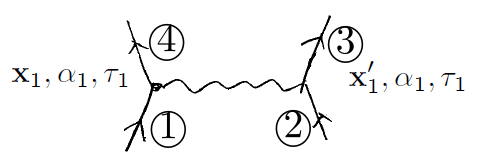
\includegraphics[width=5cm]{fig4-3-1.png}
\end{center}
where the four legs correspond to the four fields respectively, while the wavy line stands for the interaction potential.\\
With this in mind, these 6 terms can be given by these 6 Feynman diagrams respectively
%p659
\begin{center}
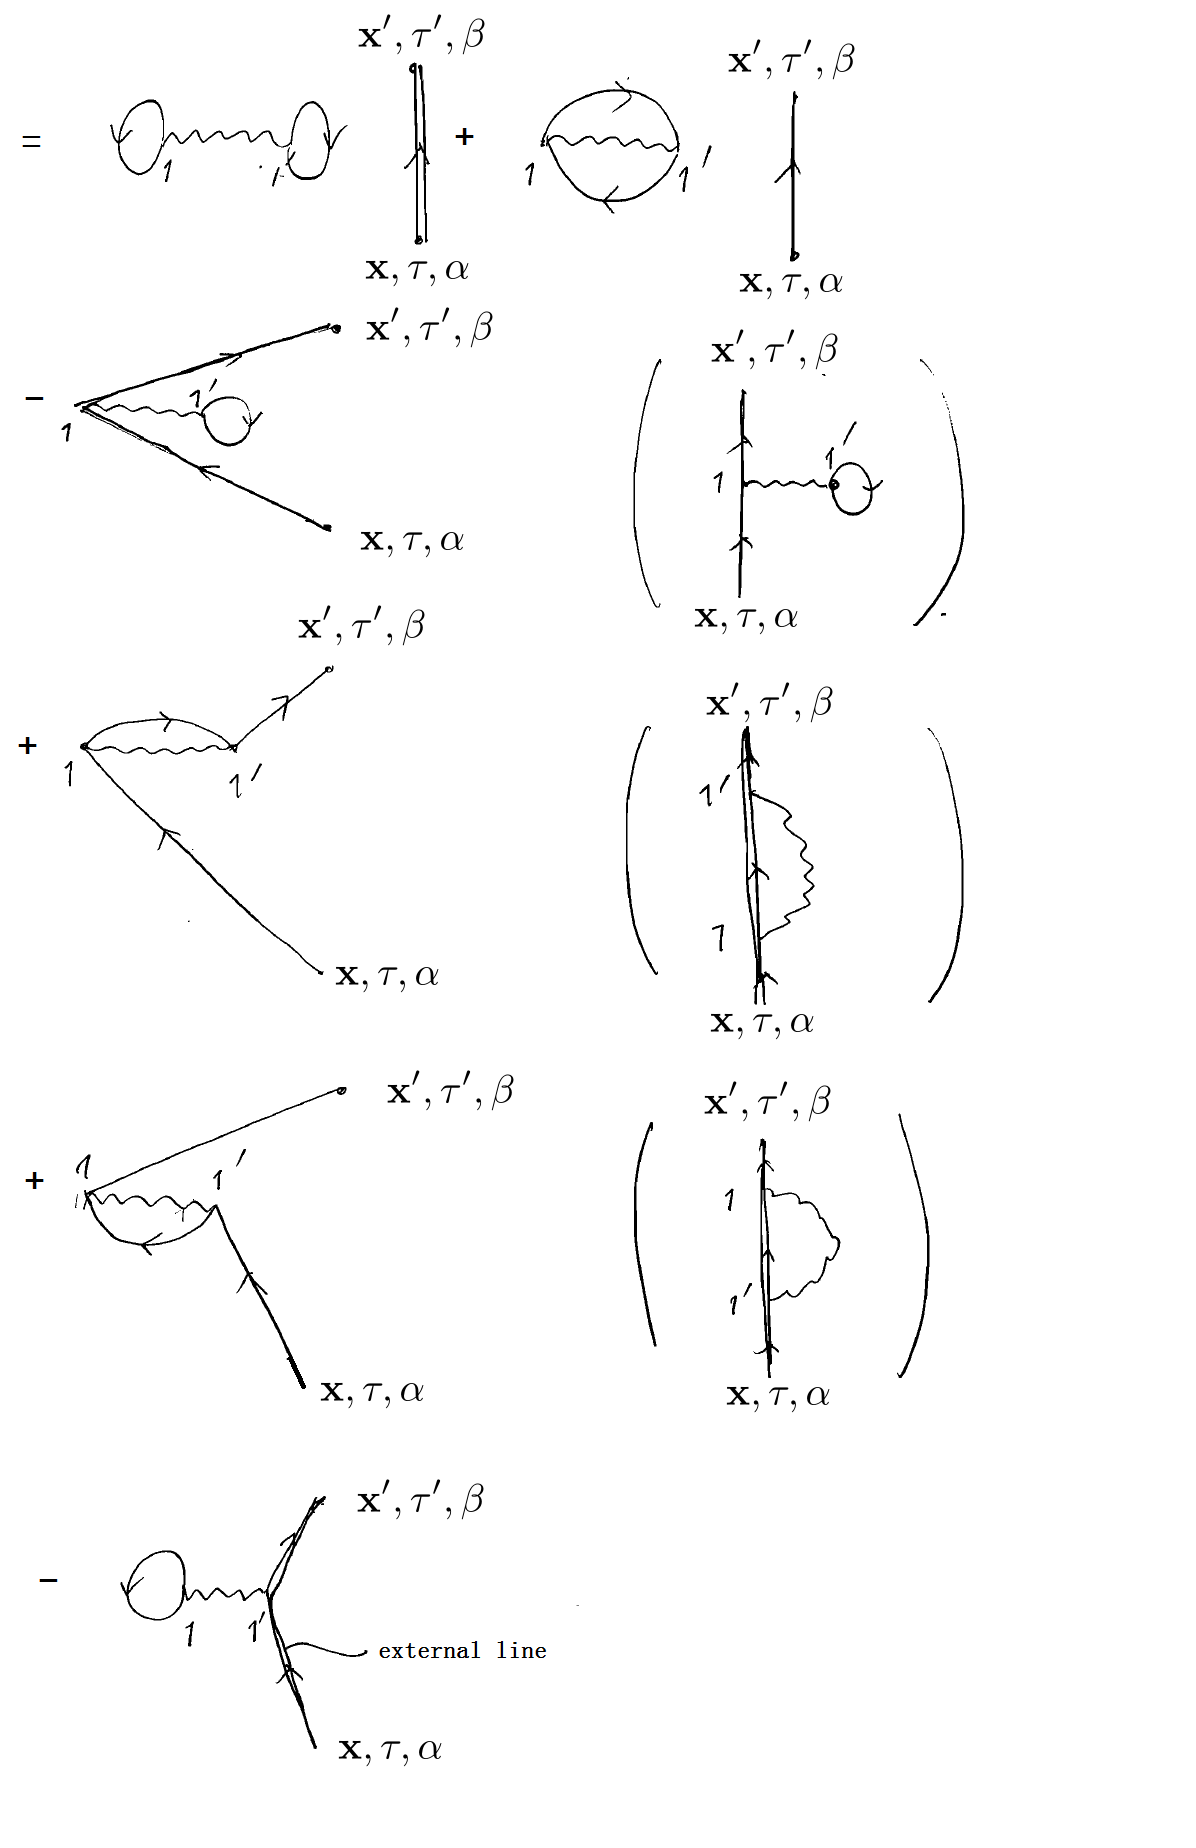
\includegraphics[height=22cm]{fig4-3-2.png}
\end{center}
%p660
We especially call that solid line which connects $\mathbf{x},\tau,\alpha$ and $\mathbf{x}',\tau',\beta$ as ``an external line''.
We call those Feynman diagram in which all the interaction potential are connected to the external line as ``connected Feynman diagram''.
%p661
For this example, the last 4 diagrams above are all connected Feynman diagram, while the first two are not.
Especially, we call these parts, which are not connected to external line, as disconnected Feynman diagram.
With this background in mind, let us go back to \ref{4.2.A}.
The $\nu-th$ order term in the numerator of \ref{4.2.A} can be rewritten as follows
%p662
$$
\begin{aligned}
\tilde{g}^{(\nu)}_{\alpha\beta}(\mathbf{x},\tau;\mathbf{x}',\tau')&\equiv \left(-\frac{1}{\hbar}\right)^\nu \frac{1}{\nu!} \int_0^{\beta\hbar}d\tau_1\cdots \int_0^{\beta\hbar}d\tau_\nu Tr\left[\rho_G^0 T_\tau\{\hat{H}_1(\tau_1) \cdots \hat{H}_1(\tau_\nu) \psi_\alpha(\mathbf{x},\tau) \psi_\beta^\dagger(\mathbf{x}',\tau')\}\right]\\
&=\left(-\frac{1}{\hbar}\right)^\nu \frac{1}{\nu!} \sum_{n=0}^\nu \frac{\nu!}{n!(\nu-n)!} \int_0^{\beta\hbar}d\tau_1\cdots \int_0^{\beta\hbar}d\tau_\nu Tr\left[\rho_G^0 T_\tau\{\hat{H}_1(\tau_1) \cdots \hat{H}_1(\tau_n)\}\right]\\
&\times Tr\left[\rho_G^0 T_\tau\{\hat{H}_1(\tau_{n+1}) \cdots \hat{H}_1(\tau_\nu) \psi_\alpha(\mathbf{x},\tau) \psi_\beta^\dagger(\mathbf{x}',\tau')\}\right]_{connected}
\end{aligned}
$$
This subscript ``connected'' means that, when taking the contraction here, we retain only those terms in which any of these interaction potentials are connected to external lines by wavy lines or solid lines.
%p663
Namely, we divide this into a product between a sum of all disconnected Feynman diagrams and a sum of all connected Feynman diagrams.
We have $\nu!/n!(n-\nu)!$ ways of dividing $\nu$ into $n$ and $n-\nu$, so that we put this factor.
When take the sum over $\nu$ from zero to infinity, we can rewrite this into.
$$
\begin{aligned}
&\sum_{\nu=0}^{+\infty}\tilde{g}^{(\nu)}_{\alpha\beta}(\mathbf{x},\tau;\mathbf{x}',\tau')\\
&=\sum_{\nu=0}^{+\infty}\left(-\frac{1}{\hbar}\right)^\nu \frac{1}{\nu!} \sum_{n=0}^\nu \frac{\nu!}{n!(\nu-n)!} \int_0^{\beta\hbar}d\tau_1\cdots \int_0^{\beta\hbar}d\tau_\nu Tr\left[\rho_G^0 T_\tau\{\hat{H}_1(\tau_1) \cdots \hat{H}_1(\tau_n)\}\right]\\
&\times Tr\left[\rho_G^0 T_\tau\{\hat{H}_1(\tau_{n+1}) \cdots \hat{H}_1(\tau_\nu) \psi_\alpha(\mathbf{x},\tau) \psi_\beta^\dagger(\mathbf{x}',\tau')\}\right]_{connected}\\
&=\sum_{n=0}^{+\infty}\left(-\frac{1}{\hbar}\right)^n \frac{1}{n!} \int_0^{\beta\hbar}d\tau_1\cdots \int_0^{\beta\hbar}d\tau_n Tr\left[\rho_G^0 T_\tau\{\hat{H}_1(\tau_1) \cdots \hat{H}_1(\tau_n)\}\right]\\
&\times\sum_{m=0}^{+\infty}\left(-\frac{1}{\hbar}\right)^m \frac{1}{m!} \int_0^{\beta\hbar}d\tau_1\cdots \int_0^{\beta\hbar}d\tau_m Tr\left[\rho_G^0 T_\tau\{\hat{H}_1(\tau_1) \cdots \hat{H}_1(\tau_n) \psi_\alpha(\mathbf{x},\tau) \psi_\beta^\dagger(\mathbf{x}',\tau')\}\right]_{connected}
\end{aligned}
$$
when substituting this into \ref{4.2.A}, the former disconnected parts are cancelled by the denominator, so that we finally obtain.
\begin{equation}\label{4.3.E}
\begin{aligned}
&g_{\alpha\beta}(\mathbf{x},\tau;\mathbf{x}',\tau')=\sum_{m=0}^{+\infty} \left(-\frac{1}{\hbar}\right)^m \frac{1}{m!} \int_0^{\beta\hbar} d\tau_1 \cdots \int_0^{\beta\hbar} d\tau_m\\
&r\left[\rho_G^0 T_\tau\{\hat{H}_1(\tau_1)\cdots\hat{H}_1(\tau_m)\psi_\alpha(\mathbf{x},\tau)\psi_\beta^\dagger(\mathbf{x}',\tau')\}\right]_{connected}
\end{aligned}
\end{equation}

\section{Feynman's rule for the temperature Green's function}

Comparing the argument so far and \ref{4.3.E}, with the zero-temperature field theory, one can see that the perturbation expansion of the temperature Green's function has the same structure as that of the zero-temperature time-ordered Green's function.
As a result, the detailed derivation of the Feynman rule is also unchanged, so that we simply summarize the Feynman rule for the single-particle temperature Green's function.\\
%p666
\uline{Fenman rule in coordinate space}

Draw all topologically distinct diagrams containing $n$ interaction lines (wavy lines) and $(2n+1)$ directed solid lines.
Assign a non-interacting temperature Green's function $g_{\alpha\beta}^0(1,2)$ for each directed solid lines. 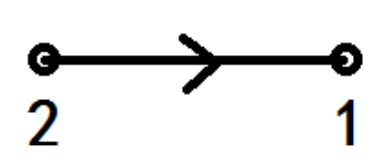
\includegraphics[height=0.7cm]{fig4-4-1.png}
Assign a factor $V(\mathbf{x}_1-\mathbf{x}_2)\delta(\tau_1-\tau_2)$ for each interaction line.\\
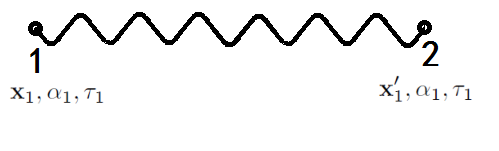
\includegraphics[height=1cm]{fig4-4-2.png}
Integrate all the internal variables $(\mathbf{x}_i,\tau_i)\ (i=1,\cdots,2n): \prod\limits_{i=1}^{2n} \int d^3 \mathbf{x}_i \int_0^{\beta\hbar} d\tau_i$
Take the sum over spin indices for internal variables: $\prod\limits_{i=1}^{2n} \sum\limits_{\alpha_i=\uparrow,\downarrow}$
Multiply each m-th-order Feynman diagram by $\left(-\frac{1}{\hbar}\right)^n (\pm1)^F$, where F is the number of closed loops formed only by solid lines. (+ is for boson and - is for fermion)
Interpret any temperature Green's function at equal time variable as

%p667
$$
g_{\alpha\beta}^0(\mathbf{x}_1,\tau_1'\mathbf{x}_2,\tau_1)=\lim_{\tau_2\rightarrow\tau_1+}g_{\alpha\beta}^0(\mathbf{x}_1,\tau_1'\mathbf{x}_2,\tau_2)
$$
\rule{\textwidth}{1mm}
For example, zero-th and 1st-order contribution to the single-particle temperature Green's function are given by these Feynman diagrams
\begin{center}
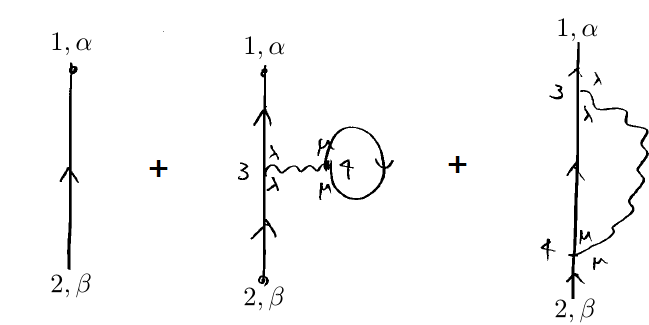
\includegraphics[height=3cm]{fig4-4-3.png}
\end{center}
%p668
According to the Feynman's rule, corresponding algebraic expression are given by
\begin{equation}
\begin{aligned}
&g_{\alpha\beta}(1,2)=g_{\alpha\beta}^0(1,2)\\
&-\hbar^{-1}\int d^3 \mathbf{x}_3 \int d^4 \mathbf{x} \int_0^{\beta\hbar} d\tau_3 \int_0^{\beta\hbar} d\tau_4
\left[\pm g_{\alpha\lambda}^0(1.3) g_{\lambda\beta}(3,2) V_0(3,4) g_{\mu\mu}^0(4,4)+ g_{\alpha\lambda}(1,3) g_{\lambda\mu}^0(3,4) g_{\mu\beta}^0(4,2) V_0(3,4)\right]\\
&+\cdots
\end{aligned}
\end{equation}
where the sign $(\pm)$ here comes from the closed loop in this diagram.
For spin-$1/2$ fermion case with spin rotational symmetry, we have
$$
g_{\alpha\beta}^0(1,2)=g^0 (1,2) \delta_{\alpha\beta}
$$
where $g^0$ is given by \ref{4.1.C}.
%p669
In such case, we have
\begin{equation}
\begin{aligned}
g_{\alpha\beta}(1,2)=&\delta_{\alpha\beta}\left\{g^0(1,2)-\hbar^{-1}\int d^3\mathbf{x}_3 \int d^3\mathbf{x}_4 \int_0^{\beta\hbar} d\tau_2 \int_0^{\beta\hbar} d\tau_4 \right.\\
& \left. \left[-2g^0(1,3)g^0(3,2)V_0(3,4)g^0(4,4)+g^0(1,3)g^0(3,4)g^0(4,2)V_0(3,4)\right]+\cdots\right\}
\end{aligned}
\end{equation}
According to the item 7 in the Feynman's rule, $g^0(4,4)$ should be interpreted as $g^0(4,4+)$, which reduces to a particle density:
\begin{equation}
\begin{aligned}
g_{\alpha\beta}^0(4,4+)&=g_{\alpha\beta}^0(\mathbf{x}_4,\tau_4;\mathbf{x}_4,\tau_4+)\\
&=-\delta_{\alpha\beta}\langle\hat{n}_\alpha(\mathbf{x}_4)\rangle_0\\
&=-\delta_{\alpha\beta} \frac{1}{2} \sum_{\alpha=\uparrow,\downarrow} \langle\hat{n}_\alpha(\mathbf{x}_4)\rangle_0\\
&=-\frac{1}{2}\delta_{\alpha\beta}\langle\hat{n}(\mathbf{x}_4)\rangle_0
\end{aligned}
\end{equation}
so that we can replace this by $-\frac{1}{2}\langle\hat{n}(\mathbf{x}_4)\rangle_0$
%p670
As in the zero-temperature field theory, it is useful to introduce the momentum space representation.
Namely, in a spatially homogenous system, the single-particle temperature Green's function depends only on the relative distance betweent two coordinates.
\begin{equation}
g_{\alpha\beta}(\mathbf{x},\tau;\mathbf{x}',\tau')=g_{\alpha\beta}(\mathbf{x}-\mathbf{x}',\tau-\tau')
\end{equation}
Thus, we can take the Fourier transformation to introduce the momentum representation.
But remember that we define $\tau$ and $\tau'$ to be within $0$ to $\beta\hbar$ $0\leq\tau,\tau'\leq\beta\hbar$, so that
\begin{equation}
-\beta\hbar\leq\tau,\tau'\leq\beta\hbar
\end{equation}
%p671
Interestingly, the temperature Green's function automatically satisfies the periodic boundary condition.
To see this, notice first that
\begin{equation}
\begin{aligned}
g_{\alpha\beta}(\mathbf{x},\beta\hbar;\mathbf{x}',\tau')&=-\frac{1}{Z_G}Tr\left[\cancel{e^{-\beta K} e^{\beta K}} e^{-K\tau'/\hbar}\psi_\alpha(\mathbf{x})e^{-\beta K} e^{K \tau'/\hbar} \psi_\beta^\dagger(\mathbf{x}')\right]\\
&=-\frac{1}{Z_G} Tr\left[e^{-\beta K} e^{K \tau'/\hbar} \psi_\beta^\dagger(\mathbf{x}')e^{-K \tau'/\hbar}\psi_\alpha(\mathbf{x})\right]\\
&=\mp g_{\alpha\beta} (\mathbf{x},0;\mathbf{x}',\tau')
\end{aligned}
\end{equation}
Similarly, we can prove that
\begin{equation}
\begin{aligned}
g_{\alpha\beta}(\mathbf{x},\tau;\mathbf{x}',\beta\hbar)&=\mp \frac{1}{Z_G} Tr\left[\cancel{e^{-\beta K} e^{\beta K}} e^{-K\tau/\hbar}\psi^\dagger_\beta(\mathbf{x}')e^{-\beta K} e^{K \tau/\hbar} \psi_\alpha (\mathbf{x})\right]\\
&=\mp\frac{1}{Z_G}Tr\left[e^{-\beta K} e^{K\tau/\hbar}\psi_\alpha(\mathbf{x}) e^{-K\tau/\hbar} \psi_\beta^\dagger(\mathbf{x}')\right]\\
&=\pm g_{\alpha\beta}(\mathbf{x},tau;\mathbf{x}',0)
\end{aligned}
\end{equation}
%p672
These two suggest that
\begin{equation}
g_{\alpha\beta}(\mathbf{x}-\mathbf{x}',-\beta\hbar\le\tau-\tau'\le0)=\pm g_{\alpha\beta}(\mathbf{x}-\mathbf{x}',0\le\tau-\tau'+\beta\hbar\le\beta\hbar)
\end{equation}
where ``+'' sign is for boson and ``-'' sign is for fermion.
This means that we can assume that the Green's function is periodic over range of $2\beta\hbar$: for both statistics.
\begin{equation}
g_{\alpha\beta}(\mathbf{x}-\mathbf{x}',\tau-\tau')=\pm g_{\alpha\beta}(\mathbf{x}-\mathbf{x}',\tau-\tau'+\beta\hbar)= g_{\alpha\beta}(\mathbf{x}-\mathbf{x}',\tau-\tau'+2\beta\hbar)
\end{equation}
With this boundary condition in mind, we will Fourier-expand the temperature Green's function as follows:
%p673
\begin{equation}
g_{\alpha\beta}(\mathbf{x}-\mathbf{x}',\tau-\tau')=\int\frac{d^3 \mathbf{k}}{(2\pi)^3} \frac{1}{\beta\hbar}\sum_n e^{i\mathbf{k}\cdot(\mathbf{x}-\mathbf{x}')} e^{-i\omega_n(\tau-\tau')} g_{\alpha\beta}(\mathbf{k},\omega_n)
\end{equation}
where
\begin{equation}
\omega_n =\frac{2n\pi}{2\beta\hbar}
\end{equation}
arbitrary integer $n$
Corresponding inverse transformation is given by
\begin{equation}
g_{\alpha\beta}(\mathbf{k},\omega_n)=\int d^3\mathbf{x}\frac{1}{2} \int_{-\beta\hbar}^{\beta\hbar} d\tau e^{-i\mathbf{k}\cdot\mathbf{x}} e^{i\omega_n\tau} g_{\alpha\beta} (\mathbf{x},\tau)
\end{equation}
Using this boundary condition, we can further rewrite this into this form.
\[
\begin{aligned}
g_{\alpha\beta}(\mathbf{k},\omega_n)&=\int d^3\mathbf{x} e^{-i\mathbf{k}\cdot\mathbf{x}} \frac{1}{2} \left(\int_{-\beta\hbar}^0 d\tau+\int_0^{\beta\hbar} d\tau\right) e^{i\omega_n\tau} g_{\alpha\beta}(\mathbf{x},\tau)\\
&=\int d^3 \mathbf{x} e^{-i\mathbf{k}\cdot\mathbf{x}} \frac{1}{2} \int_0^{\beta\hbar} d\tau \left\{e^{i\omega_n(\tau-\beta\hbar)}g_{\alpha\beta}(\mathbf{x},\tau-\beta\hbar)+e^{i\omega_n\tau}g_{\alpha\beta}(\mathbf{x},\tau)\right\}\\
&=\int d^3\mathbf{x} e^{-i\mathbf{k}\cdot\mathbf{x}}\frac{1}{2} \int_0^{\beta\hbar} d\tau \left\{\pm e^{in\pi}+1\right\}e^{i\omega_n\tau}g_{\alpha\beta}(\mathbf{x},\tau)
\end{aligned} \tag{$4.4.12^\prime$}
\]
This suggests that, for boson case, the Fourier coefficient becomes non-zero only when $n$ is even integer, while for fermion case, the coefficient becomes non-zero only when $n$ is odd integer.\\
\uline{boson}
$$
g_{\alpha\beta}(\mathbf{k},\omega_n)=
\begin{cases}
\int d^3 \mathbf{x} e^{-i\mathbf{k}\cdot\mathbf{x}}\int_0^{\beta\hbar} d\tau e^{i\omega_n\tau} g_{\alpha\beta}(\mathbf{x},\tau)&(n=even)\\
0&(n=odd)
\end{cases}
$$
\uline{fermion}
$$
g_{\alpha\beta}(\mathbf{k},\omega_n)=
\begin{cases}
\int d^3 \mathbf{x} e^{-i\mathbf{k}\cdot\mathbf{x}}\int_0^{\beta\hbar} d\tau e^{i\omega_n\tau} g_{\alpha\beta}(\mathbf{x},\tau)&(n=odd)\\
0&(n=even)
\end{cases}
$$
To summarize, the Fourier series of the temperature Green's function is given by
\begin{equation}
g_{\alpha\beta}(\mathbf{k},\omega_n)=\int d^3\mathbf{x} e^{-i\mathbf{k}\cdot\mathbf{x}} int_0^{\beta\hbar} e^{i\omega_n\tau}g_{\alpha\beta}(\mathbf{x},\tau)
\end{equation}
\begin{equation}
\omega_n\equiv
\begin{cases}
\frac{2n\pi}{\beta\hbar} &(boson)\\
\frac{(2n+1)\pi}{\beta\hbar} &(fermion)
\end{cases}
\end{equation}
\begin{equation}
g_{\alpha\beta}(\mathbf{x},\tau)=\int \frac{d^3\mathbf{k}}{(2\pi)^3} \frac{1}{\beta\hbar} \sum_m e^{i\mathbf{k}\cdot\mathbf{x}} e^{-i\omega_m\tau}g_{\alpha\beta}(\mathbf{k},\omega_m)
\end{equation}
This discrete frequency is often called as Matsubara frequency.
%p676
As an example, let us consider Fourier series of the non-interacting temperature Green's function.
\begin{equation}
\begin{aligned}
g^0(\mathbf{k},\omega_n)&\equiv \int d^3\mathbf{x} e^{-i\mathbf{k}\cdot\mathbf{x}} \int_0^{\beta\hbar} d\tau e^{i\omega_n\tau} g^0(\mathbf{x},\tau)\\
&=-\frac{1}{V}\sum_{\mathbf{k}'} \int d^3\mathbf{x} e^{-i\mathbf{k}\cdot\mathbf{x}} \int_0^{\beta\hbar} d\tau e^{i\omega_n\tau} e^{i\mathbf{k}'\cdot\mathbf{x}-\frac{\epsilon^0_{k'}-\mu}{\hbar}} \left(1\pm n_{k'}^0\right)\\
&=-\sum_{\mathbf{k}'} \delta_{\mathbf{k},\mathbf{k}'} \frac{1}{i\omega_n-\frac{\epsilon^0_{k'}-\mu}{\hbar}}\left[e^{i\omega_n-\frac{\epsilon^0_{k'}-\mu}{\hbar}}\right]_{\tau=0}^{\tau=\beta\hbar}(1\pm n_{k'}^0)\\
&=-\frac{1}{i\omega_n-\frac{\epsilon^0_{k'}-\mu}{\hbar}}\left[\cancelto{\pm1}{e^{i\omega_n\beta\hbar}} e^{-(\epsilon_k^0-\mu)\beta}-1\right] (1\pm n_k^0)\\
&=-\frac{1}{i\omega_n-\frac{\epsilon^0_{k'}-\mu}{\hbar}}\left[\pm1 e^{-(\epsilon_k^0-\mu)\beta}-1\right] \frac{e^{-(\epsilon_k^0-\mu)\beta}}{e^{-(\epsilon_k^0-\mu)\beta\mp1}}\\
&=\frac{1}{i\omega_n-\frac{\epsilon^0_{k'}-\mu}{\hbar}}
\end{aligned}
\end{equation}
%p677
With these preliminaries in mind, it is now straightforward to derive the Feynman rules in the momentum space.
The derivation goes exactly in parallel with the zero-temperature field theory, so that I will describe only the results in the following.
Feynman rules for the n-th order contribution to $g_{\alpha\beta}(\mathbf{k},\omega_n)$.
Draw all topologically distinct connected graphs with n interaction lines (wavy lines) and (2n+1) directed particle lines (solid lines).
%p678
Assign a direction to each interaction line. Associate a wave vector and discrete Matsubara frequency with each interaction line and particle line and conserve momentum and frequency at each vertex\\
\begin{center}
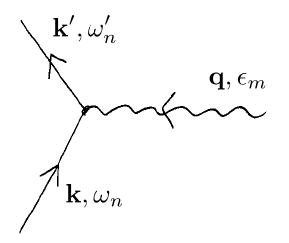
\includegraphics[height=3cm]{fig4-4-4.png}
\end{center}
$$
\left\{
\begin{aligned}
&\mathbf{k}'=\mathbf{k}+\mathbf{q}\\
&\omega_n'=\omega_n+\epsilon_m
\end{aligned}
\right.
$$
For each particle line (solid line), assign a non-interacting temperature Green's function
\[
g_{\alpha\beta}^0(\mathbf{}k,\omega_n)=\frac{\delta_{\alpha\beta}}{i\omega_n-\hbar^{-1}(\epsilon_k^0-\mu)}
\]
where $\omega_n=\frac{2n\pi}{\beta\hbar}$ for boson, while $\omega_n=\frac{(2n+1)\pi}{\beta\hbar}$
For an interaction line, assign $V(\mathbf{q})$ (free from frequency)
Now we have n independent internal wave vectors and frequencies
\[
\underset{\#(particl\ lines)}{(2n+1)}+\underset{\#(interaction\ lines)}{n}-\underset{\begin{aligned}&\#(vertex)\\&=\#(conservation)\end{aligned}}{2n}-\underset{\begin{aligned}&external\ momentum\\&and\ frequency\end{aligned}}{1}=n
\]
Integrate over all the n independent internal wave vectors and frequencies:
\[
\prod_{j=1}^{n}\left(\int d^3\mathbf{k}_j\sum_{\omega_j}\right)
\]
Spin indices of the Green's function for a matrix product along any continuous particle lines which share a same vertex should be taken to be same. Under this condition, take the sum over all spin indices.
Multiply by $\left(-\frac{1}{\hbar}\cdot\frac{1}{\beta\hbar}\cdot\frac{1}{(2\pi)^3}\right)(\pm1)^F$, where F is the number of closed loops formed by continuous particle lines (+ is for boson, - is for fermion)
%p680
When a particle line closes on itself 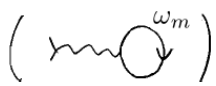
\includegraphics[height=0.7cm]{fig4-4-5.png} or a particle line joined by the same interaction line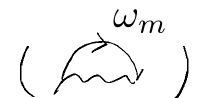
\includegraphics[height=1cm]{fig4-4-6.png}, assign a convergence factor $e^{i\omega_m\eta}$ for particle line.\\
\rule{\textwidth}{1mm}

As an example, consider again the zero-th and first order contribution to the single-particle temperature Green's function.
\begin{center}
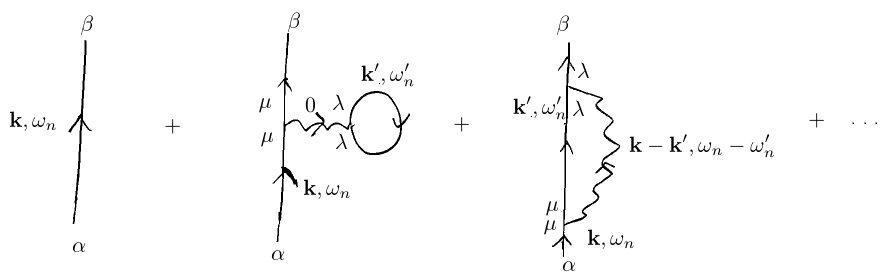
\includegraphics[height=3cm]{fig4-4-7.png}
\end{center}
\begin{equation}
\begin{aligned}
g_{\alpha\beta}(\mathbf{k},\omega_n)&=g_{\alpha\beta}^0(\mathbf{k},\omega_n)-\frac{1}{\hbar}\int\frac{d\mathbf{k}'}{(2\pi)^3}\frac{1}{\beta\hbar} \sum_{\omega_n'} e^{i\omega_n'\eta}\\
&\times\left\{\pm g_{\alpha\mu}(\mathbf{k},\omega_n)g_{\mu\beta}(\mathbf{k},\omega_n) V(0) g_{\lambda\lambda}(\mathbf{k}',\omega_n')+ g_{\alpha\mu}(\mathbf{k},\omega_n) g_{\mu\lambda}(\mathbf{k}',\omega_n') g_{\lambda\beta}(\mathbf{k},\omega_n) V(\mathbf{k}-\mathbf{k}')\right\}\\
&+\cdots
\end{aligned}
\end{equation}
%p681
For spin $-1/2$ fermion case with spin rotational symmetry, we can take
\[
g_{\alpha\beta}^0(\mathbf{k},\omega_n)=\delta_{\alpha\beta}^0(\mathbf{k},\omega_n)
\]
so that we have
\[
g_{\alpha\beta}(\mathbf{k},\omega_n)=\delta(\mathbf{k},\omega_n)
\]
\begin{equation}
\begin{aligned}
g(\mathbf{k},\omega_n)&=g^0(\mathbf{k},\omega_n)-\frac{1}{\hbar}\int\frac{d\mathbf{k}'}{(2\pi)^3}\frac{1}{\beta\hbar} \sum_{\omega_n'} e^{i\omega_n'\eta}\\
&\times\left\{-2\left[g(\mathbf{k},\omega_n)\right]^2 V(0) g(\mathbf{k}',\omega_n')+ \left[g(\mathbf{k},\omega_n)\right]^2 V(\mathbf{k}-\mathbf{k}') g(\mathbf{k}',\omega_n) \right\}\\
&+\cdots
\end{aligned}
\end{equation}
where we took `-' sign for the fermion.
The factor `2' comes from the summation over spin index $(\lambda)$.
As in the zero-temperature field theory,$g(\mathbf{k},\omega_n)$ can be expressed in terms of self energy
%p682
\begin{equation}
g(\mathbf{k},\omega_n)=g^0(\mathbf{k},\omega_n)+g^0(\mathbf{k},\omega_n)\sigma (\mathbf{k},\omega_n) g^0(\mathbf{k},\omega_n)
\end{equation}
where the first order contribution to the self-energy is given by
\begin{equation}
\Sigma^{(1)}(\mathbf{k},\omega_n)=-\frac{1}{\hbar}\int \frac{d\mathbf{k}'}{(2\pi)^3} \uline{\frac{1}{\beta\hbar} \sum_{\omega_n'} e^{i\omega_n\eta} g^0(\mathbf{k},\omega_n)}\cdot\left(-2V(0)+V(\mathbf{k}-\mathbf{k}')\right)
\end{equation}
Frequency summation in the underlined part is a typical summation, which we will encounter in finite-temperature field theory.
Thus, we will demonstrate how to take this discrete sum, for the fermion case.
\begin{equation}
\frac{1}{\beta\hbar} \sum_{\omega_n'} e^{i\omega_n\eta} \frac{1}{i\omega_n'-\hbar^{-1}(\epsilon_k^0-\mu)}
\end{equation}
For simplicity, we take this real-value quantity $\hbar^{-1}(\epsilon^{0}_{k'}-\mu)$ to be x and replace $\omega^{\prime}_n$ by $\omega_n$.
\[
\frac{1}{\beta\hbar}\sum_{\omega_n}e^{i\omega_n\eta} \frac{1}{i\omega_n-x} \tag{$4.4.21^\prime$}
\]
%p683
Now that this single-particle temperature Green's function is for fermion, $\omega_n$ is restricted to be $(2n+1)\pi/\beta\hbar$
\[
\omega_b=\frac{(2n+1)\pi}{\beta\hbar}\qquad(n:integer)
\]
To evaluate this sum we introduce a complex variable $z$, which corresponds to $i\omega_n$. Then, the sum over $\omega_n$ can be generally given by
\begin{equation}
\frac{1}{\beta\hbar}\sum_{\omega_n}f(i\omega_n)=-\oint\frac{dz}{2\pi i}\frac{1}{e^{\beta\hbar z}+1}f(z)
\end{equation}
where the contour integral in the right hand side is taken along a loop which encloses the imaginary axis in the complex z-plane.
%p683
\[
Im\ z\ \Gamma\ \frac{\pi i}{\beta\hbar}\ \frac{3\pi i}{\beta\hbar}\ \frac{5\pi i}{\beta\hbar}\ \frac{7\pi i}{\beta\hbar}\ \frac{-\pi i}{\beta\hbar}\ \frac{-3\pi i}{\beta\hbar}\ Re\ z
\]
\begin{center}
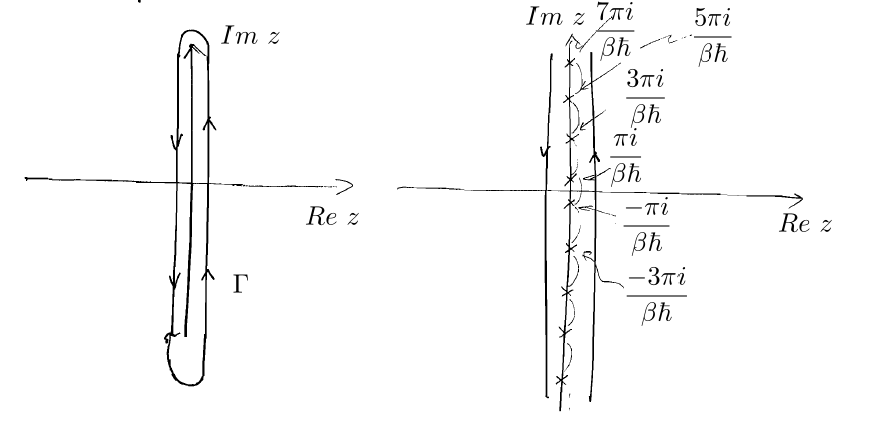
\includegraphics[height=4cm]{fig4-4-8.png}
\end{center}
To see this formula, notice first that $\frac{1}{e^{\beta\hbar z}+1}$ has a pole at $z=\frac{(2n+1)\pi}{\beta\hbar}i$ where $n$ is arbitrary integer.
Therefore, when $f(z)$ has no pole inside this closed loop, we can split this closed loop into a infinite number of small loops, each of which encloses each of these poles.
%p685
\begin{center}
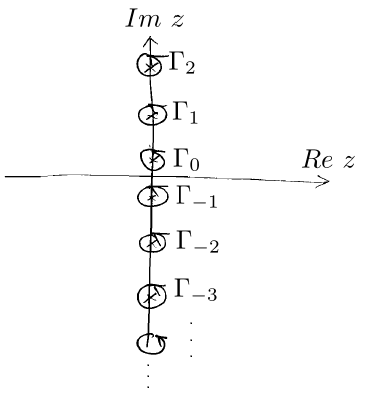
\includegraphics[height=4cm]{fig4-4-9.png}
\end{center}
\[
\begin{aligned}
&-\oint_\Gamma \frac{dz}{2\pi i} \frac{1}{e^{\beta\hbar z}+1}f(z)\\
&=-\sum_n \oint \frac{d\Delta z}{2\pi i} \frac{f(i\omega_n)}{e^{\beta\hbar(i\omega_n+\Delta z)}+1}\\
&=\frac{1}{\beta\hbar} \sum_n \oint_{\Gamma_n} \frac{d\Delta z}{2\pi i} \frac{1}{\Delta z} f(i\omega_n)\\
&=\frac{1}{\beta\hbar}\sum_n f(i\omega_n) \frac{1}{e^{\beta\hbar(i\omega_n+\Delta z)}+1}\\
&=\frac{1}{e^{(2n+1)\pi+\beta\hbar\Delta z}+1}\\
&=\frac{1}{-e^{\beta\hbar z}+1}\\
&=\frac{1}{\beta\hbar z}
\end{aligned}
\]
From this derivation, one might also notice that this function $\frac{1}{e^{\beta\hbar z}+1}$ can be replaced by other functions which have poles at $z=i\omega_n$.
For example, we can also express this sum by this complex integral.
\[
\frac{1}{\beta\hbar}\sum_{\omega_n}f(i\omega_n)=\oint_\Gamma \frac{dz}{2\pi i} \frac{1}{1+e^{-\beta\hbar z}}f(z) \tag{$4.4.22^\prime$}
\]
Whether we should choose this or the other depends on an asymptotic behavior of a function f(z) in $|z|\rightarrow+\infty$
In the present situation, f(z) is given by this
\[
f(z)=\frac{e^{z\eta}}{z-x}
\]
which reduces to zero for $Re\ z\rightarrow-\infty$ while diverges for $Re\ z\rightarrow+\infty$ because $\eta$ is an infinitesimally small positive value.
In such case, we choose the former one, because the underlined integrand reduces to zero both for $Re\ z\rightarrow-\infty$ and $Re\ z\rightarrow+\infty$
\[
\frac{1}{\beta\hbar}\sum_{\omega_n}f(i\omega_n)=-\oint_\Gamma\frac{dz}{2\pi i} \uline{\frac{1}{1+e^{\beta\hbar z}}\frac{e^{z\eta}}{z-x}}
\]
where
\[
\begin{cases}
\frac{1}{1+e^{\beta\hbar z}}\frac{e^{z\eta}}{z-x}\rightarrow 0 & Re\ z\rightarrow+\infty\quad(\beta\hbar\gg\eta> 0)\\
\frac{1}{1+e^{\beta\hbar z}}\frac{e^{z\eta}}{z-x}\rightarrow 0 & Re\ z\rightarrow-\infty
\end{cases}
\]
%o688
This asymptotic behavior allows us to put two infinitely large contours: one is in the region of $Re\ z> 0$ and the other is in the region of $Re\ z< 0$.
\begin{center}
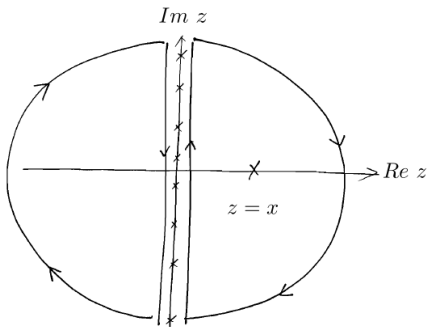
\includegraphics[height=4cm]{fig4-4-10.png}
\end{center}
Now that the integrand has a pole only on the real axis, we can deform in this way
\begin{center}
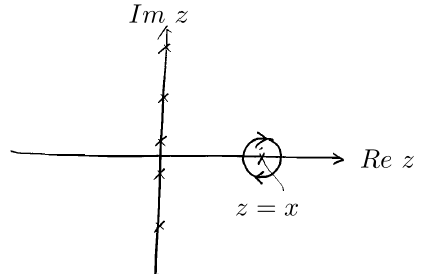
\includegraphics[height=4cm]{fig4-4-11.png}
\end{center}
%p689
Correspondingly, this integral is evaluated as follows
\begin{equation}
-\oint_\Gamma\frac{dz}{2\pi i} \frac{1}{1+e^{\beta\hbar z}}\frac{e^{z\eta}}{z-x}=\frac{1}{e^{\beta\hbar x}+1}
\end{equation}
Namely, we have
\[
\frac{1}{\beta\hbar}\sum_{\omega_n} e^{i\omega_n\eta} \frac{1}{i\omega_n-\hbar^{-1}(\epsilon_k^0-\mu)}=\frac{1}{e^{\beta(\epsilon_k^0-\mu)}+1}=n_k^0\ (fermi distribution function) \tag{$4.4.23^\prime$}
\]
using this evaluation, the first-order self energy is now simplified into.
\begin{equation}
\Sigma^{(1)} (\mathbf{k},\omega_n)=-\frac{1}{\hbar} \int \frac{d^3\mathbf{k}}{(2\pi)^3} n_{k'}^0 \left(-2V(0)+V(\mathbf{k}-\mathbf{k}')\right)
\end{equation}
At the zero-temperature, this reduces to 2.5.9, because $n_{k'}^0=\theta(k_F-|\mathbf{k}|)$

\section{Dyson's equation \& Hartree-Fock approximation}
\subsection{Dyson equations for the temperature Green's function}

Temperature Green's function consists of an identical set of Feynman diagram as the zero-temperature Green's function.
Thus, it is quite natural that the same Dyson's equation holds true for the temperature Green's function.
In coordinate space, the single-particle temperature Green's function always has the form:
\begin{equation}
g(1,2)=g^0(1,2)+\int d3\int d4 g^0(1,3)\Sigma(3,4)g^0(4,2)
\end{equation}
where the integral contains not only the integral over the space coordinate but also the sum over spin index and the time integration over $0$ to $\beta\hbar$
%p691
\[
\int d3=\int d^3 \mathbf{x}_3 \int_0^{\beta\hbar} \sum_{\alpha_3}
\]
This defines the total self-energy $\Sigma(3,4)$.
As in the zero-temperature field theory, it is also useful to define the `proper' self-energy $\Sigma^\star(3,4)$, which consistes of all self-energy diagram, that cannot be decomposed into two parts by cutting only one particle lines $g^0$.
When a self-energy diagram is decomposed into several parts like this.
\[
\tilde{\Sigma}(1,2)=\int d3\cdots\int d7 \Sigma_a^\star(1,3)g^0(3,4)\Sigma_b^\star(4,5)\cdots g^0(6,7)\tilde{\Sigma}_c^\star(7,2)
\]
the factor $(-1/\hbar)^n(\pm1)^F$ appearing in the item 6 of the Feynman rule can be also decomposed into each of these proper self-energy.
%p692
\[
(-1/\hbar)^n(\pm1)^F=(-1/\hbar)^{n_a}(\pm1)^{F_a}\cdot(-1/\hbar)^{n_b}(\pm1)^{F_b}\cdots\cdot(-1/\hbar)^{n_c}(\pm1)^{F_c}
\]
\[
with
\left(
\begin{aligned}
n&=n_a+n_b+\cdots+n_c\\
F&=F_a+F_b+\cdots+F_c
\end{aligned}
\right)
\]
As such, the exact single-particle temperature Green's function is given only by the proper self-energy as follows
\begin{equation}
\begin{aligned}
g(1,2)&=g^0(1,2)+\int d3\int d4 g^0(1,3) \Sigma^\star(3,4) g^0(4,2) +\int d3 d4 d5 d6 g^0(1,3)\Sigma^\star(3,4) g^0(4,5) \Sigma^\star(5,6) g^0(6,2)+\cdots\\
&=g^0(1,2) +\int d3 d4 g^0(1,3)\Sigma^\star(3,4) g(4,2)
\end{aligned}
\end{equation}
%p693
which we call Dyson's equation.
As in the zero-temperature field theory, the Dyson's equation reduces to an algebraic equation in the momentum-frequency representation:
\begin{equation}
g(\mathbf{k},\omega_n)=g^0(\mathbf{k},\omega_n)+g^0(\mathbf{k},\omega_n)\Sigma^\star(\mathbf{k},\omega_n)g(\mathbf{k},\omega_n)
\end{equation}
where we assume the spin rotational symmetry for simplicity.
Here the Fourier series of the self-energy is defined as
\begin{equation}
\Sigma^\star(\mathbf{k},i\omega_n)=\int_0^{\beta\hbar} d\tau \int d^3\mathbf{x} e^{-i\mathbf{k}\cdot\mathbf{x}+i\omega_n\tau}\Sigma^\star(\mathbf{x},\tau)
\end{equation}
where the self-energy depends only on the relative coordinate for spatially homogeneous system,
\[
\left.
\begin{aligned}
\Sigma^\star(\mathbf{x},\tau)&\equiv\Sigma^\star(\mathbf{x}_3,\tau_3;\mathbf{x}_4,\tau_4)\\
with\ \mathbf{x}&\equiv\mathbf{x}_3-\mathbf{x}_4\\
\tau&\equiv\tau_3-\tau_4
\end{aligned}
\right\}\tag{$4.5.4^\prime$}
\]
This algebraic equation can be explicitly solved for the Green'f function
\begin{equation}
g(\mathbf{k},\omega_n)=\frac{1}{g^0(\mathbf{k},\omega_n)-\Sigma^\star(\mathbf{k},\omega_n)}
\end{equation}
or equivalently, we have
\[
g(\mathbf{k},\omega_n)=\frac{\delta_{\alpha\beta}}{i\omega_n-\hbar^{-1}(\epsilon_k^0-\mu)-\Sigma^\star(\mathbf{k},\omega_n)}\tag{$4.5.5^\prime$}
\]
$\star$ Hatree-Fock approximation
Self-consistent Hatree-Fock approximation at the zero-temperature field theory can be also generalized into the finite-temperature field theory.
We begin with the first order perturbation to the proper self-energy
\begin{center}
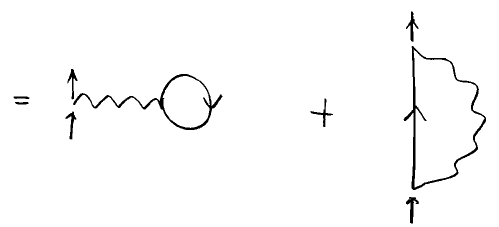
\includegraphics[height=2cm]{fig4-5-1.png}
\end{center}
%p695
in which these internal particle lines are non-interacting Green's function.
In the (self-consistent) Hatree-Fock approximation, we replace these non-interacting Green's functions by the exact Green's function.
\begin{center}
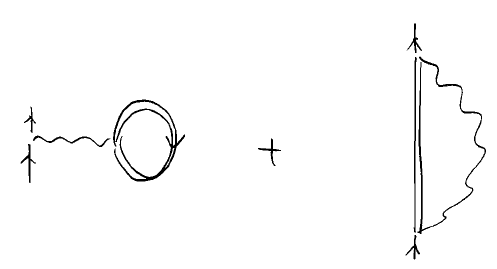
\includegraphics[height=2cm]{fig4-5-2.png}
\end{center}
To concretize this approximation, let us consider a system in a static spin-independent external potential $U(\mathbf{x})$.
\begin{equation}
\left\{
\begin{aligned}
\hat{K}_0&=\int d^3 \mathbf{x} \hat{\psi}_\alpha^\dagger(\mathbf{x}) \left[-\frac{\hbar^2\nabla_x^2}{2m}+U_0(\mathbf{x})-\mu\right] \hat{\psi}_\alpha(\mathbf{x})\\
\hat{H}_1&=\int d^3 \mathbf{x} \int d^3 \mathbf{x}' \hat{\psi}_\alpha^\dagger(\mathbf{x}) \hat{\psi}_\beta^\dagger(\mathbf{x}') V(\mathbf{x}-\mathbf{x}') \hat{\psi}_\beta(\mathbf{x}')\hat{\psi}_\alpha(\mathbf{x})
\end{aligned}
\right.
\end{equation}
%p696
For simplicity, we assume the spin-rotational symmetry, so that the Green's function is diagonal with respect to the spin index.
\begin{equation}
g_{\alpha\beta}(\mathbf{x},\tau;\mathbf{x}',\tau')\equiv\delta_{\alpha\beta}g(\mathbf{x},\tau;\mathbf{x}',\tau')
\end{equation}
The Dyson equation for the Green's function is given by
\begin{equation}
\begin{aligned}
g(\mathbf{x},\tau;\mathbf{x}',\tau')=&g^0(\mathbf{x},\tau;\mathbf{x}',\tau')\\&+\int d^3 \mathbf{x}_1 \int d^3 \mathbf{x}_1' \int_0^{\beta\hbar}d\tau_1 \int_0^{\beta\hbar}d\tau_1' g^0(\mathbf{x},\tau;\mathbf{x}_1,\tau_1) \Sigma^\star(\mathbf{x}_1,\tau_1;\mathbf{x}_1',\tau_1') g(\mathbf{x}_1',\tau_1';\mathbf{x}',\tau')
\end{aligned}
\end{equation}
According to the Feynman's rule, the first-order perturbational contribution to the proper self-energy is given by
%p697
\begin{equation}
\begin{aligned}
\Sigma^\star(\mathbf{x}_1,\tau_1;\mathbf{x}_1',\tau_1')=&-\frac{1}{\hbar}\left[\pm(2s+1)\delta^3(\mathbf{x}_1-\mathbf{x}_1')\delta(\tau_1-\tau_1')\int d^3 \mathbf{x}_2 V(\mathbf{x}_1-\mathbf{x}_2) g(\mathbf{x}_2,\tau_1;\mathbf{x}_2,\tau_1+)\right.\\
&\left.+\delta(\tau_1-\tau_1') g(\mathbf{x}_1,\tau_1;\mathbf{x}_1',\tau_1+) V(\mathbf{x}_1-\mathbf{x}_2)\right]
\end{aligned}
\end{equation}
\rule{\textwidth}{1mm}
\[
\begin{aligned}
\because &\int d^3 \mathbf{x}_1 \int d^3 \mathbf{x}_1' \int_0^{\beta\hbar} d\tau_1 \int_0^{\beta\hbar} d\tau_1' g^0(\mathbf{x},\tau;\mathbf{x}_1,\tau_1) \Sigma^\star(\mathbf{x}_1,\tau_1;\mathbf{x}_1',\tau_1') g^0(\mathbf{x}_1',\tau_1';\mathbf{x}',\tau')\\
&=-\frac{1}{\hbar} \left[\pm(2s+1)\int d^3 \mathbf{x}_1 \int_0^{\beta\hbar} d\tau_1 g^0(\mathbf{x},\tau;\mathbf{x}_1,\tau_1) g^0(\mathbf{x},\tau;\mathbf{x}',\tau')\times\int d^3 \mathbf{x}_2 V(\mathbf{x}_1-\mathbf{x}_2) g^0(\mathbf{x}_2,\tau_1;\mathbf{x}_2,\tau_1+)\right]\\
&\quad-\frac{1}{\hbar} \int d^3 \mathbf{x}_1 \int d^3 \mathbf{x}_1' \int_0^{\beta\hbar} d\tau_1 \int_0^{\beta\hbar} d\tau_1' g^0(\mathbf{x},\tau;\mathbf{x}_1,\tau_1) g^0(\mathbf{x}_1,\tau_1;\mathbf{x}_1',\tau_1') \delta(\tau_1-\tau_1') V(\mathbf{x}_1-\mathbf{x}_2) g^0(\mathbf{x}_1',\tau_1';\mathbf{x}',\tau')
\end{aligned}
\]
\rule{\textwidth}{1mm}\\
Within the Hatree-Fock approximation, we replace these non-interacting Green's function by the exact Green's function.
%p698
Irrespective of the presence of homogeneous external potential $U(\mathbf{x})$, we can still Fourier transform the time variable into Matsubara frequency.
\begin{equation}
g(\mathbf{x},\tau;\mathbf{x}',\tau')=g(\mathbf{x},\mathbf{x}';\tau-\tau')=\frac{1}{\beta\hbar}\sum_n e^{-i\omega_n(\tau-\tau')} g(\mathbf{x},\mathbf{x}';\omega_n)
\end{equation}
where
$
\omega_n=
\begin{cases}
\frac{2n\pi}{\beta\hbar} & (for\ boson)\\
\frac{(2n+1)\pi}{\beta\hbar} & (for\ fermion)
\end{cases}
$
The same fourier transformation is applicable to the self-energy, so that we have
\begin{equation}
\Sigma^\star(\mathbf{x},\tau;\mathbf{x}',\tau')=\frac{1}{\beta\hbar}\sum_n e^{-i\omega_n(\tau-\tau')} \Sigma^\star(\mathbf{x},\mathbf{x}';\omega_n)
\end{equation}
with $
\omega_n=
\begin{cases}
\frac{2n\pi}{\beta\hbar} & (for\ boson)\\
\frac{(2n+1)\pi}{\beta\hbar} & (for\ fermion)
\end{cases}
$\\
%p699
Under this transformation, the Dyson equation and self-consistent Hatree-Fock equation become as follows respectively.
\[
\begin{aligned}
g(\mathbf{x},\mathbf{x}';\omega_n)=&g^0(\mathbf{x},\mathbf{x}';\omega_n)+\int_0^{\beta\hbar} d(\tau-\tau') e^{i\omega_n(\tau-\tau')} \int d^3\mathbf{x}_1 \int d^3\mathbf{x}_1' \int_0^{\beta\hbar} d\tau_1 \int_0^{\beta\hbar} d\tau_1'\\
&\frac{1}{\beta\hbar}\sum_{\omega_1} e^{-i\omega_1(\tau-\tau_1)} g^0(\mathbf{x},\mathbf{x}_1;\omega_1)\\
&\times\frac{1}{\beta\hbar}\sum_{\omega_2} e^{-i\omega_2(\tau_1-\tau_1')} \Sigma^\star(\mathbf{x}_1,\mathbf{x}_1';\omega_2)\\
&\times\frac{1}{\beta\hbar}\sum_{\omega_3} e^{-i\omega_3(\tau_1'-\tau')} g^0(\mathbf{x}_1',\mathbf{x}';\omega_3)
\end{aligned}
\]
Note that
\[
\int_0^{\beta\hbar} d\tau_1 e^{i(\omega_1-\omega_2)\tau_1}=\beta\hbar\delta_{n_1,n_2}
\]
\[
\int_0^{\beta\hbar} d\tau_1' e^{i(\omega_2-\omega_3)\tau_1'}=\beta\hbar\delta_{n_2,n_3}
\]
\[
\int_0^{\beta\hbar} d(\tau-\tau') e^{i(\omega_n-\omega_1)(\tau-\tau')}=\beta\hbar\delta_{n,n_1}\\
\]
%p700
\[
g(\mathbf{x},\mathbf{x}';\omega_n)=g^0(\mathbf{x},\mathbf{x}';\omega_n)+\int d^3\mathbf{x}_1\int d^3\mathbf{x}_1' g(\mathbf{x},\mathbf{x}_1;\omega_n) \Sigma^\star(\mathbf{x}_1,\mathbf{x}_1';\omega_n) g(\mathbf{x}_1',\mathbf{x}';\omega_n)
\]
\begin{equation}\label{eq4.5.12}
\begin{aligned}
\Sigma^\star(\mathbf{x}_1,\mathbf{x}_1';\omega_n)=&-\frac{1}{\hbar}\Big [\pm(2s+1)\delta^3(\mathbf{x}_1-\mathbf{x}-1')\\
&\times\int d^3\mathbf{x}_2 V(\mathbf{x}_1-\mathbf{x}_2)\frac{1}{\beta\hbar} \sum_{\omega_m} g(\mathbf{x}_1,\mathbf{x}_2;\omega_m)e^{i\omega_m\eta}\\
&+\frac{1}{\beta\hbar}\sum_{\omega_m}g(\mathbf{x}_1,\mathbf{x}_1';\omega_m)e^{i\omega_m\eta}V(\mathbf{x}_1-\mathbf{x}_1')\Big ]
\end{aligned}
\end{equation}
where the self-energy is independent of the Matsubara frequency, so that we simply rewrite it as:
\[
\Sigma^\star(\mathbf{x}_1,\mathbf{x}_1';\omega_n)=\Sigma^\star(\mathbf{x}_1,\mathbf{x}_1')
\]
The non-interacting Green's function can be expanded in terms of the eigen wavefunction of single-particle Hamiltonian.
%p701
Suppose that the single-particle Hamiltonian is diagonalized by $\psi_j^0(\mathbf{x})$ with its eigen value $\epsilon_j^0$.
\begin{equation}
\left[-\frac{\hbar^2\nabla^2}{2m}+U(\mathbf{x})-\mu\right]\psi_j^0(\mathbf{x})=(\epsilon_j^0-\mu)\psi_j^0(\mathbf{x})
\end{equation}
In terms of this single-particle basis, the field operator is expanded as follows
\begin{equation}
\left\{
\begin{aligned}
\psi_\alpha(\mathbf{x})&=\sum_j\psi_j^0(\mathbf{x})a_{j,\alpha}\\
\psi_\alpha^\dagger(\mathbf{x})&=\sum_j\psi_j^{0*}(\mathbf{x})a^\dagger_{j,\alpha}
\end{aligned}
\right.
\end{equation}
where the completeness of the basis is represented by the following equation:
\begin{equation}\label{eq4.5.16}
\sum_j\psi_j^0(\mathbf{x})\psi_j^{0*}(\mathbf{x})=\delta^3(\mathbf{x}-\mathbf{x}')
\end{equation}
while the orthogonality is represented by
\begin{equation}
\int d^3\mathbf{x} \psi_j^{0*}(\mathbf{x})\psi_m^0(\mathbf{x}) \delta_{j,m}
\end{equation}
%p702
In terms of this basis, $\hat{K_0}$ is given by
\begin{equation}
\hat{K_0}=\sum_{j,\alpha}(\epsilon_j^0-\mu)a_{j,\alpha}^\dagger a_{j,\alpha}
\end{equation}
Non-interacting temperature Green's function is given by
\[
\begin{aligned}
g_{\alpha\beta}^0(\mathbf{x},\tau;\mathbf{x}',\tau')&=-e^{\beta\Omega_0}Tr\left[e^{-\beta\hat{K}_0} T_\tau\{\hat{\psi}_{K_0\alpha}(\mathbf{x},\tau) \hat{\psi}_{K_0\beta}^\dagger(\mathbf{x}',\tau')\}\right]\\
&=-\left\{\theta(\tau-\tau')\langle\hat{\psi}_{K_0\alpha}(\mathbf{x},\tau)\hat{\psi}_{K_0\beta}^\dagger(\mathbf{x}',\tau')\right\}
\end{aligned}
\]
where 
\[
\begin{aligned}
\hat{\psi}_{k_0\alpha}(\mathbf{x},\tau) & \equiv e^{\hat{k_0}\tau/\hbar} \hat{\psi}_\alpha(\mathbf{x}) e^{-\hat{k_0}\tau/\hbar}\\
&=\sum_j e^{-(\epsilon^0_j-\mu)\tau/\hbar} \phi^0_j(\mathbf{x}) a_{j,\alpha}\\
\hat{\psi}_{k_0\beta}^\dag(\mathbf{x}',\tau')&=\sum_j e^{(\epsilon^0_j-\mu)\tau'/\hbar} \phi^{0\star}_j(\mathbf{x}') a_{j,\alpha}
\end{aligned}
\]
%p703
Using these two, we have
\[
\langle \hat{\psi}_{k_0\alpha}(\mathbf{x},\tau) \hat{\psi}_{k_0\beta}^\dag(\mathbf{x}',\tau')\rangle_0
=\sum_{j,m}e^{-(\epsilon^0_j-\mu)\tau/\hbar} e^{(\epsilon^0_m-\mu)\tau'/\hbar} \phi_j^0(\mathbf{x})\phi_m^{0\star}(\mathbf{x}) \langle a_{j,\alpha}a^\dag_{m,\beta}\rangle_0
\]

\[
\begin{aligned}
\langle a_{j,\alpha}a^\dag_{m,\beta}\rangle_0&=\delta_{j,m}\delta_{\alpha\beta} \langle a_{j,\alpha}a^\dag_{j,\alpha}\rangle_0\\
&=\delta_{j,m}\delta_{\alpha\beta}(1\pm \langle a^\dag_{j,\alpha}a_{j,\alpha}\rangle_0\\
&=\delta_{j,m}\delta_{\alpha\beta} (1\pm n^0_{j,\alpha})
\end{aligned}
\]

\[
\langle \hat{\psi}_{k_0\alpha}(\mathbf{x},\tau) \hat{\psi}_{k_0\beta}^\dag(\mathbf{x}',\tau')\rangle_0
=\sum_{j}e^{-(\epsilon^0_j-\mu)(\tau-\tau')/\hbar} \phi_j^0(\mathbf{x})\phi_j^{0\star}(\mathbf{x}') \delta_{\alpha\beta} (1\pm n^0_{j,\alpha})
\]
Similarly, we have
\[
\langle \hat{\psi}_{k_0\beta}^\dag(\mathbf{x}',\tau') \hat{\psi}_{k_0\alpha}(\mathbf{x},\tau)\rangle_0
=\sum_{j}e^{-(\epsilon^0_j-\mu)(\tau-\tau')/\hbar} \phi_j^0(\mathbf{x})\phi_j^{0\star}(\mathbf{x}')\delta_{\alpha\beta} n^0_{j,\alpha}
\]
%p704
Using these two, we have
\begin{equation}
g_{\alpha\beta}^0(\mathbf{x},\tau;\mathbf{x}',\tau')=-\delta_{\alpha\beta}\sum_j e^{-(\epsilon^0_j-\mu)(\tau-\tau')/\hbar} \phi_j^0(\mathbf{x})\phi_j^{0\star}(\mathbf{x}') \left\{ \theta(\tau-\tau') (1 \pm n^0_{j,\alpha}) \pm \theta(\tau'-\tau)n_{j,\alpha}^0 \right\}
\end{equation}
whose Fourier series is given by
\[
g_{\alpha\beta}^0(\mathbf{x},\mathbf{x}';\omega_n)=\delta_{\alpha\beta}g^0(\mathbf{x},\mathbf{x}';\omega_n)
\]
\[
\begin{aligned}
g^0(\mathbf{x},\mathbf{x}';\omega_n)&=\int^{\beta\hbar}_0 d(\tau-\tau')e^{i\omega_n(\tau-\tau')}g^0_{\alpha\beta}(\mathbf{x},\tau;\mathbf{x}',\tau')\\
&=-\sum_j \phi_j^0(\mathbf{x})\phi_j^{0\star}(\mathbf{x}') \int^{\beta\hbar}_0 d\tau e^{(i\omega_n-(\epsilon-\mu)/\hbar) \tau} (1\pm n^0_{j,\alpha})\\
&=-\sum_j \phi_j^0(\mathbf{x})\phi_j^{0\star}(\mathbf{x}') \frac{\pm e^{(-\epsilon_j^0-\mu)\beta}-1}{i\omega_n-(\epsilon-\mu)/\hbar } (1\pm n^0_{j,\alpha})
\end{aligned}
\]
%p705
\[
1\pm n^0_{j,\alpha}=\frac{ e^{(-\epsilon_j^0-\mu)\beta}\mp1 \pm 1}{ e^{(-\epsilon_j^0-\mu)\beta}\mp1}=\frac{1}{ 1\mp e^{(-\epsilon_j^0-\mu)\beta}}
\]
\begin{equation}
g^0(\mathbf{x},\mathbf{x}';\omega_n)=\sum_j \frac{\phi_j^0(\mathbf{x})\phi_j^{0\star}(\mathbf{x}')}{i\omega_n-(\epsilon_j-\mu)/\hbar}
\end{equation}
In a similar way, let us assume that the interacting temperature Green's function can be also expanded in terms of a certain single-particle basis, which will be justified as posteriori within the self-consistent Hartree-Fock approximation,
\begin{equation}\label{eq4.5.21}
g(\mathbf{x},\mathbf{x}';\omega_n)=\sum_j \frac{\phi_j(\mathbf{x})\phi_j^{\star}(\mathbf{x}')}{i\omega_n-(\epsilon_j-\mu)/\hbar}
\end{equation}
where we remove the superscript ``0''.
%p706
Substituting this form into eq.(\ref{eq4.5.12}) , we have the proper self-energy within the Hartree-Fock approximation as follows:
\[
\begin{aligned}
\hbar \Sigma^\star(\mathbf{x}_1,\mathbf{x}_1')
=&\mp (2s+1)\delta^3 (\mathbf{x}_1,\mathbf{x}_1') \int d^3\mathbf{x}_2 V(\mathbf{x}_1-\mathbf{x}_2)\frac{1}{\beta\hbar} \sum_{\omega_m} e^{i\omega_m\eta}\sum_j \frac{\phi_j(\mathbf{x_1})\phi_j^{\star}(\mathbf{x_2})}{i\omega_m-(\epsilon_j-\mu)/\hbar}\\
&+V(\mathbf{x}_1-\mathbf{x}_1')\frac{1}{\beta\hbar} \sum_{\omega_m} e^{i\omega_m\eta}\sum_j \frac{\phi_j(\mathbf{x_1})\phi_j^{\star}(\mathbf{x_1'})}{i\omega_m-(\epsilon_j-\mu)/\hbar}
\end{aligned}
\]
where ``-'' sign is for boson and ``+\\ sign is for fermion.
For each case, the Matsubara frequency is defined as follows
\[
\omega_m=\left\{
\begin{aligned}
&\frac{2m\pi}{\beta\hbar}\qquad (boson)\\
&\frac{(2m+1)\pi}{\beta\hbar}\qquad (fermion)
\end{aligned}
\right.
\]
%p707
In either case, we can evaluate this summation by the complex integral as we didi for fermion case before.
The result becomes as follows
\[
\frac{1}{\beta\hbar} \sum_{\omega_m} e^{i\omega_m\eta} \frac{1}{i\omega_m-(\epsilon_j-\mu)/\hbar}=\mp \frac{1}{e^{\beta(\epsilon_j-\mu)}\mp1}\equiv \mp n_j
\]
where $\eta > 0$
Substituting this into these two parts, we finally reach the following expression for the proper self-energy:
\begin{equation}\label{eq4.5.22}
\hbar \Sigma^\star(\mathbf{x}_1,\mathbf{x}_1')
=\mp (2s+1)\delta^3 (\mathbf{x}_1,\mathbf{x}_1') \int d^3\mathbf{x}_2 V(\mathbf{x}_1-\mathbf{x}_2) \sum_j |\phi_j(\mathbf{x})|^2n_j\mp V(\mathbf{x}_1-\mathbf{x}_1')\sum_j \phi_j(\mathbf{x_1})\phi_j^{\star}(\mathbf{x_1'})n_j
\end{equation}
%p708
To justify that the interacting Green's function can be expanded in terms of a certain single-particle basis, let us apply the following differential operator onto the Dyson's equation from the left hand side:
\begin{equation}
\mathscr{L}_1(x,\nabla x)=\i\hbar \omega_n - \left( -\frac{\hbar^2\nabla^2_\mathbf{x}}{2m}+U(\mathbf{x}-\mu)\right)
\end{equation}
\[
\mathscr{L}_1(x,\nabla x) g(\mathbf{x},\mathbf{x}';\omega_n)=\mathscr{L}_1(x,\nabla x) \left[ g^0(\mathbf{x},\mathbf{x}';\omega_n)+\int d^3\mathbf{x}_1 \int d^3\mathbf{x}_1' g^0(\mathbf{x},\mathbf{x}_1;\omega_n)\Sigma^\star (\mathbf{x}_1,\mathbf{x}_1')g(\mathbf{x}_1',\mathbf{x}';\omega_n)\right]
\]
Note that
%p709
\begin{equation}\label{eq4.5.24}
\begin{aligned}
\mathscr{L}_1(x,\nabla x) g^0(\mathbf{x},\mathbf{x}';\omega_n)
&=\left[i\hbar \omega_n - \left( -\frac{\hbar^2\nabla^2_\mathbf{x}}{2m}+U(\mathbf{x}-\mu)\right) \right] \sum_j \frac{\phi_j^0(\mathbf{x})\phi_j^{0\star}(\mathbf{x'})}{i\omega_m-(\epsilon_j^0-\mu)/\hbar}\\
&=\hbar sum_j \phi_j^0(\mathbf{x})\phi_j^{0\star}(\mathbf{x'})=\hbar \delta^3 (\mathbf{x}-\mathbf{x}')
\end{aligned}
\end{equation}
where we use $\left( -\frac{\hbar^2\nabla^2_\mathbf{x}}{2m}+U(\mathbf{x}-\mu)\right)\phi_j^0 (\mathbf{x})=(\epsilon_j^0-\mu) \phi_j^0(\mathbf{x})$, the completeness of $\{ \phi_j^0\}$ and eq.(\ref{eq4.5.16}) in the final line.\\
Using this, we can rewrite this into
\begin{equation}
\mathscr{L}_1(x,\nabla x) g(\mathbf{x},\mathbf{x}';\omega_n)=\hbar \delta^3(\mathbf{x}-\mathbf{x}')+\int d^3\mathbf{x}_1\int d^3\mathbf{x}_1'\hbar \delta^3(\mathbf{x}-\mathbf{x}_1)\Sigma^\star (\mathbf{x}_1,\mathbf{x}_1')g(\mathbf{x}_1',\mathbf{x}';\omega_n)
\end{equation}
By transferring the 2nd term into the left hand side, we have
%p710
\begin{equation}\label{eq4.5.26}
\left[i\hbar \omega_n - \left( -\frac{\hbar^2\nabla^2_\mathbf{x}}{2m}+U(\mathbf{x}-\mu)\right) \right] g(\mathbf{x},\mathbf{x}';\omega_n)+\int d \mathbf{x}^{\prime \prime} \Sigma^\star (\mathbf{x},\mathbf{x}^{\prime\prime})g(\mathbf{x}^{\prime\prime},\mathbf{x}';\omega_n)=\hbar \delta^3(\mathbf{x}-\mathbf{x}')
\end{equation}
Such an equation is satisfied by eq.(\ref{eq4.5.21}), if and only if the single-particle basis is an eigen wavefunction of the following linear operator:
\begin{equation}\label{eq4.5.27}
\int d^3 \mathbf{x}' \mathscr{L}(\mathbf{x},\mathbf{x}')\phi_j(\mathbf{x}')=\epsilon_j\phi_j(\mathbf{x}')
\end{equation}
where
\begin{equation}\label{eq4.5.28}
\mathscr{L}(\mathbf{x},\mathbf{x}')=\delta^3(\mathbf{x}-\mathbf{x}')\left[ -\frac{\hbar^2\nabla^2_\mathbf{x}}{2m}+U(\mathbf{x}) \right]+ \Sigma^\star (\mathbf{x},\mathbf{x}')
\end{equation}
Generally speaking, we can expect that such an eigen wavefunction constitutes a complete set; so that we have 
\begin{equation}\label{eq4.5.29}
\sum_j\phi_j(\mathbf{x}) \phi_j^\star(\mathbf{x}')=\delta^3(\mathbf{x}-\mathbf{x}')
\end{equation}
%p711
Then using eq.(\ref{eq4.5.27}), eq.(\ref{eq4.5.28}) and eq.(\ref{eq4.5.29}), we can prove eq.(\ref{eq4.5.26}) exactly in the same way as we did in eq.(\ref{eq4.5.24}).
To summerize, eq(\ref{4.5.22}) and eq(\ref{eq4.5.27},\ref{eq4.5.28}) comprise a set of self-consistent equation for unknown set of functions $\{ \phi_j(\mathbf{x})\}$ and unknown set of eigenvalues $\{ \epsilon_j\}$.
This set of equation is a generalisation of Hartree-Fock approximation at finite temperature.
In a spatially homogeneous system, where $U(\mathbf{x})=0$, this set of self consistent equation becomes simplified.
%p712
In such a case, the self-energy depends only on the relative coordinate
\[
\Sigma^\star(\mathbf{x},\mathbf{x}')=\Sigma^\star(\mathbf{x}-\mathbf{x}')
\]
Thus, we have only to choose the plane wave for $\phi_j(\mathbf{x})$
\[
\phi_j(\mathbf{x})\rightarrow \frac{1}{\sqrt{V}}e^{i\mathbf{k} \cdot \mathbf{x}}
\]
Then eq.(\ref{eq4.5.28}) reduces to 
\begin{equation}
\frac{\hbar^2 \mathbf{k}^2}{2m}+\Sigma^\star (\mathbf{k})=\epsilon_{\mathbf{k}}
\end{equation}
with $\Sigma^\star (\mathbf{k})=\int d^3(\mathbf{x}-\mathbf{x}') e^{-i\mathbf{k}\cdot (\mathbf{x}-\mathbf{x'})} \Sigma^\star (\mathbf{x}-\mathbf{x}')$
On the other hand, eq(\ref{eq4.5.22}) reduces to 
\begin{equation}
\hbar \Sigma^\star (\mathbf{k})=(2s+1)V(0)\int \frac{d^3\mathbf{k}'}{(2\pi)^3} n'_\mathbf{k}\mp\int \frac{d^3\mathbf{k}'}{(2\pi)^3} V(\mathbf{k}-\mathbf{k}') n'_k
\end{equation}
%p713
with 
\begin{equation}\tag{4.5.30$^\prime$}
n_k=\frac{1}{e^{\beta(\epsilon_k-\mu)}+1}
\end{equation}
Namely, we have only to solve the following self-consistent equation
\begin{equation}\label{eq4.5.31}
\left\{
\begin{aligned}
\epsilon_k&=\frac{\hbar^2 k^2}{2m}+\hbar\Sigma^\star(\mathbf{k})\\
\hbar \Sigma^\star(\mathbf{k})&=(2s+1)V(0)\int\frac{d^3\mathbf{k}'}{(2\pi)^3}n_k'\mp\int\frac{d^3\mathbf{k}'}{(2\pi)^3}V(\mathbf{k}-\mathbf{k}')n_k'
\end{aligned}
\right.
\end{equation}
%




\section{Specific heat of an imperfect Fermi gas at low-temperature}
%
As an example of the Hartree-Fock approximation, let us evaluate the entropy and specific heat of an imperfect Fermi gas in the low-temperature limit.
%p714
In the grand canonical ensemble, the thermodynamic potential is given as a function of temperature, volume and chemical potential.
\begin{equation}
\Omega(T,V,\mu)=E(T,V,\mu)-TS(T,V,\mu)-\mu N(T,V,\mu)
\end{equation}
where
\begin{equation}\label{eq4.6.2}
S(T,V,\mu)=-\left( \frac{\partial\Omega}{\partial T}\right)_{V,\mu}
\end{equation}
\begin{equation}
N(T,V,\mu)=-\left( \frac{\partial\Omega}{\partial \mu}\right)_{V,T}
\end{equation}
Solving the latter equation inversely, we can express the chemical potential as a function of $T,V$ and $N$
\[
N=N(T,V,\mu)
\]
\[
\rightarrow \mu=\mu(T,V,N)
\]
Substituting this into the former equation, the entropy is given as a function of $T,V \& N$
\[
S(T,V,\mu)=S(T,V,\mu(T,V,N))
\]
%p715
from which we can evaluate the specific heat as 
\begin{equation}
C_V=T\left(\frac{\partial S}{\partial T}\right)_{V,N}
\end{equation}
To obtain the total number of fermions as a function of $T,\ V$ and $\mu$ microscopically, we go back to eq.(\ref{eq4.1.7})
\begin{equation}\label{eq4.6.5}
\begin{aligned}
N(T,V,\mu)&=\int d^3 \mathbf{x} \langle n(\mathbf{x})\rangle\\
&=\int d^3 \mathbf{x} tr[g(\mathbf{x},\tau,\mathbf{x},\tau+)]\\
&=V\int \frac{d^3\mathbf{k}}{(2\pi)^3} \frac{1}{\beta\hbar}\sum_n e^{i\omega_n\eta} tr[g(\mathbf{k},\omega_n)]
\end{aligned}
\end{equation}
To obtain the entropy as a function of $T,\ V$ and $\mu$, we need to calculate the thermodynamic potential $\Omega$ in terms of Green's function.
In fact, eq(\ref{eq4.1.18}) gives the thermodynamic potential in terms of the single particle temperature Green's function.
%p716
However, such an evaluation requires an integral over an auxiliary parameter $\lambda$, which is a bit cumbersome.
On the one hand, eq.(\ref{eq4.1.14}), let us first define a following ``thermodynamic function'' $K$ as a function of $T,\ V$ and $A$
\begin{equation}
K(T,V,\mu)=E(T,V,\mu)-\mu N(T,V,\mu)=\Omega(T,V,\mu)+TS(T,V,\mu)
\end{equation}
%p717
The first derivative of $K$ with respect to temperature with fixed $V$ and $\mu$ is calculated as follows:
\[
\left( \frac{\partial K}{\partial T}\right)_{V,\mu}=\left( \frac{\partial \Omega}{\partial T}\right)_{V,\mu}+S(T,V,\mu)+T\left( \frac{\partial S}{\partial T}\right)_{V,\mu}
\]
Using eq.(\ref{eq4.6.2}), the first two terms in R.H.S vanish.\\
So that we have
\begin{equation}
\left( \frac{\partial K}{\partial T}\right)_{V,\mu}=T\left( \frac{\partial s}{\partial T}\right)_{V,\mu}
\end{equation}
Accordingly, by integrating this equation with respect to the temperature with fixed $V$ and $\mu$, we have the entropy as a function of $V$ \& $\mu$
\begin{equation}
s(T,V,\mu)=\cancelto{0}{S(T=0,V,\mu)}+\int_0^T\frac{1}{T'}\left( \frac{\partial K}{\partial T'}\right)_{V,\mu} dT'
\end{equation}
%p718
Thus, the remaining task is to evaluate the thermodynamic function $K$ as a function of $T,\ V$ \& $\mu$.
eq.(\ref{4.1.14}) suggests that the internal energy is given by
\[
\langle E \rangle=-\frac{1}{2}\int d^3\mathbf{x} \lim_{\tau'\to \tau+} \lim_{\mathbf{x}'\to\mathbf{x}}\left(\hbar \partial_\tau +\frac{\hbar^2\nabla^2_\mathbf{x}}{2m}-\mu\right) Tr[g(\mathbf{x},\tau;\mathbf{x}',\tau')]
\]
with $g(\mathbf{x},\tau;\mathbf{x}',\tau')\equiv\int \frac{d^3\mathbf{k}}{(2\pi)^3}\frac{1}{\beta\hbar}\sum_n e^{i\mathbf{k}\cdot(\mathbf{x}-\mathbf{x}')-i\omega_n(\tau-\tau')}g(\mathbf{k},\omega_n)$
we have 
\begin{equation}\label{eq4.6.9}
\begin{aligned}
\langle E \rangle&=-\frac{1}{2}\int d^3 \mathbf{x} \lim_{\tau'\to \tau+} \lim_{\mathbf{x}'\to\mathbf{x}} \int \frac{d^3 \mathbf{k}}{(2\pi)^3} \frac{1}{\beta\hbar} \sum_n e^{i\omega_n \eta}\left(-i\hbar\omega_n-\frac{\hbar^2\mathbf{k}^2}{2m}-\mu\right)g(\mathbf{k},\omega_n)\\
&=-\frac{V}{2} \int \frac{d^3 \mathbf{k}}{(2\pi)^3} \frac{1}{\beta\hbar} \sum_n e^{i\omega_n \eta}\left(-i\hbar\omega_n-\frac{\hbar^2\mathbf{k}^2}{2m}-\mu\right)g(\mathbf{k},\omega_n)\\
&=\frac{V}{2} \int \frac{d^3 \mathbf{k}}{(2\pi)^3} \frac{1}{\beta\hbar} \sum_n e^{i\omega_n \eta}\left(i\hbar\omega_n+\frac{\hbar^2\mathbf{k}^2}{2m}+\mu\right)g(\mathbf{k},\omega_n)
\end{aligned}
\end{equation}
%p719
Summing eq(\ref{eq4.6.9}) and eq(\ref{eq4.6.5}) we have the thermodynamic function $K$ in terms of Green's fn.
\begin{equation}\label{eq4.6.10}
\langle K \rangle=\langle E \rangle-\mu\langle N \rangle=\frac{V}{2} \int \frac{d^3 \mathbf{k}}{(2\pi)^3} \frac{1}{\beta\hbar} \sum_n e^{i\omega_n \eta}\left(i\hbar\omega_n+\epsilon_K^0-\mu\right)Tr g(\mathbf{k},\omega_n)
\end{equation}
Within the Hartree-Fock approximation, the temperature Green's function $g(\mathbf{k},\omega_n)$ is given by
\begin{equation}
g(\mathbf{k},\omega_n)=\frac{1}{i\omega_n-\hbar^{-1}(\epsilon_k-\mu)}
\end{equation}
where 
\[
n_k=\frac{1}{e^{\beta(\epsilon_k-\mu)}+1}
\]
and
\[
\begin{aligned}
\epsilon_k&=\frac{\hbar^2 k^2}{2m}+\hbar\Sigma^\star(\mathbf{k})\\
\hbar \Sigma^\star(\mathbf{k})&=2V(0)\int\frac{d^3\mathbf{k}'}{(2\pi)^3}n_k'-\int\frac{d^3\mathbf{k}'}{(2\pi)^3}V(\mathbf{k}-\mathbf{k}')n_k'
\end{aligned}
\]
%p720
Such a green's function depends on temperature through $\omega_n$, because $\omega=\frac{(2n+1)\pi}{\beta\hbar}$.
But it also depends on temperature through $\epsilon_k$, because the Hartree-Fock self-energy $\Sigma^\star(\mathbf{k})$ depends on the temperature through the Fermi distribution function.
In order to distinguish these two temperature dependence from each other, we put another argument to the Green's function
\[
g(\mathbf{k},\omega_n)\to g(\mathbf{k},\omega_n,\uline{T})
\]
where this (underlined) temperature-dependence comes only from that of $\epsilon_k$.
For example,
%p721
\begin{equation}
g(\mathbf{k},\omega_n,\uline{T})=\frac{1}{i\omega_n-\hbar^{-1}(\epsilon_k-\mu)}
\end{equation}
with
\begin{equation}\tag{4.6.13$^\prime$}
\left\{
\begin{aligned}
\epsilon_k&=\epsilon_k^0+\hbar\Sigma^\star(\mathbf{k})\\
\hbar \Sigma^\star(\mathbf{k})&=2V(0)\int\frac{d^3\mathbf{k}'}{(2\pi)^3} \theta(k_F-|\mathbf{k}'|)-\int\frac{d^3\mathbf{k}'}{(2\pi)^3}V(\mathbf{k}-\mathbf{k}') \theta(k_F-|\mathbf{k}'|)
\end{aligned}
\right.
\end{equation}
With this notation in mind, let us evaluate the right-hand-side of eq(\ref{eq4.6.10}), using the low-temperature expansion.
\begin{equation}\tag{4.3.10}
\langle K \rangle=\langle E \rangle-\mu\langle N \rangle=\frac{V}{2} \int \frac{d^3 \mathbf{k}}{(2\pi)^3} \frac{1}{\beta\hbar} \sum_n e^{i\omega_n \eta}\left(i\hbar\omega_n+\epsilon_K^0-\mu\right)Tr g(\mathbf{k},\omega_n,T)
\end{equation}
where
\[
\begin{aligned}
g^{-1}(\mathbf{k},\omega_n,T)&=i\omega_n -\hbar^{-1} (\epsilon_k(T)-\mu)\\
&=i\omega_n -\hbar^{-1} (\epsilon_k^0-\mu) - \Sigma^\star(\mathbf{k},T)\\
&=g^{0-1}(\mathbf{k},\omega_n)-\Sigma^\star(\mathbf{k},T=0)+(\Sigma^\star(\mathbf{k},T)- \Sigma^\star(\mathbf{k},T=0))\\
&=g^{-1}(\mathbf{k},\omega_n,T=0)+(\Sigma^\star(\mathbf{k},T)-\Sigma^\star(\mathbf{k},T=0))
\end{aligned}
\]
%722
Equivalently, we have
\begin{equation}
g(\mathbf{k},\omega_n,T)=g(\mathbf{k},\omega_n,T=0)+g(\mathbf{k},\omega_n,T=0) (\Sigma^\star(\mathbf{k},T)-\Sigma^\star(\mathbf{k},T=0)) g(\mathbf{k},\omega_n,T)
\end{equation}
For sufficiently low-temperature, we can expand this T-dependence, iteratively in small $\Sigma^\star(\mathbf{k},T)-\Sigma^\star(\mathbf{k},T=0)$
\begin{equation}\label{eq4.6.15}
g(\mathbf{k},\omega_n,T)=g(\mathbf{k},\omega_n,T=0)+g(\mathbf{k},\omega_n,T=0) (\uline{\Sigma^\star(\mathbf{k},T)-\Sigma^\star(\mathbf{k},T=0)}) g(\mathbf{k},\omega_n,T)+O(T^2)
\end{equation}
%p723
In the following, we will evaluate the leading order T-dependence in this underlined part.
According to eq.(\ref{eq4.5.31}) the self-energy is given by a self consistent equation
\begin{equation}\label{eq4.6.16}
\begin{aligned}
\Sigma^\star(\mathbf{k})&=2V(0)\int\frac{d^3\mathbf{k}'}{(2\pi)^3}n_k'-\int\frac{d^3\mathbf{k}'}{(2\pi)^3}V(\mathbf{k}-\mathbf{k}')n_k'\\
n_k&=\frac{1}{e^{\beta(\epsilon_k-\mu)}+1}
\end{aligned}
\end{equation}
with
\begin{equation}
\epsilon_k(T)=\epsilon_k^0+\hbar \Sigma^\star (\mathbf{k},T)
\end{equation}
Thus, the temperature dependence of the self-energy comes not only from ($\beta$) but also from the \uline{the temperature dependence of $\epsilon_k$}, latter of which is nothing but the temperature dependence of the self-energy itself.
%p724
To distinguish these two temperature dependence from each other, let us define
\begin{equation}
\epsilon_k(0) = \epsilon_k^0+\hbar \Sigma^\star (\mathbf{k},T=0)
\end{equation}
Then we can formally expand $n_k$ around $\epsilon_k(T)=\epsilon_k(0)+\hbar( \Sigma^\star (\mathbf{k},T)-\Sigma^\star (\mathbf{k},T=0))$
Namely, we have
\begin{equation}
n_k=n_k(T) + \frac{\partial n_k(T)}{\partial \epsilon_k} \hbar ( \Sigma^\star (\mathbf{k},T)-\Sigma^\star (\mathbf{k},T=0))+O(T^2)
\end{equation}
Here we define $n_k(T)$, which is different from $n_k$, because its temperature dependence stems only from $\beta$, while $\epsilon_k$ is evaluated at $T=0$.
Substituting this into eq.(\ref{eq4.6.16}), we have
%p725
\begin{equation}
\begin{aligned}
\hbar \Sigma^\star (\mathbf{k},T)&=\int \frac{d^3 \mathbf{q}}{(2\pi)^3} [2V(0)-V(\mathbf{k}-\mathbf{q})] n_q\\
&\approx \int \frac{d^3 \mathbf{q}}{(2\pi)^3} [2V(0)-V(\mathbf{k}-\mathbf{q})]\left\{ n_q(T)+\frac{\partial n_q(T)}{\partial \epsilon_q} \hbar ( \Sigma^\star (\mathbf{q},T)-\Sigma^\star (\mathbf{q},0))\right\}
\end{aligned}
\end{equation}
Subtracting this by its $T=0$ evaluation, we reach a self-consistent integral eq. for $\Sigma^\star (\mathbf{k},T)-\Sigma^\star (\mathbf{k},T=0)$
\begin{equation}
\Sigma^\star (\mathbf{k},T)-\Sigma^\star (\mathbf{k},0)\approx \int \frac{d^3 \mathbf{q}}{(2\pi)^3} [2V(0)-V(\mathbf{k}-\mathbf{q})]\left\{ (n_q(T)-n_q(0)) +\frac{\partial n_q(T)}{\partial \epsilon_q} \hbar ( \Sigma^\star (\mathbf{q},T)-\Sigma^\star (\mathbf{q},0))\right\}
\end{equation}
where
\begin{equation}
\hbar \Sigma ^\star (\mathbf{k},0)=\int \frac{d^3 \mathbf{q}}{(2\pi)^3} [2V(0)-V(\mathbf{k}-\mathbf{q})]n_k(0)
\end{equation}
%p726
The thermodynamic function $K(T,V,\mu)$ can be obtained by the substitution of eq(\ref{eq4.6.15}) into eq(\ref{eq4.6.10}) 
\begin{equation}
\langle K\rangle=V\int \frac{d^3 \mathbf{k}}{(2\pi)^3} \frac{1}{\beta\hbar} \sum_n e^{i\omega_n \eta} (i\hbar \omega_n+\epsilon_k^0-\mu)\left\{ g(\mathbf{k},\omega_n,T=0) +g^2(\mathbf{k},\omega_n,T=0) \int \frac{d^3 \mathbf{q}}{(2\pi)^3} [2V(0)-V(\mathbf{k}-\mathbf{q})]\right\}
\end{equation}
As we did before, the summations over the Matsubara frequency are evaluated in terms of the complex integrals.

\[
\begin{aligned}
\frac{1}{\beta\hbar} \sum_n e^{i\omega_n \eta} \frac{i\hbar \omega_n+\epsilon_k^0-\mu}{i\omega_n-\hbar^{-1}(\epsilon_k(0)-\mu)}
&=-\int\frac{1}{e^{\beta\hbar z}+1} e^{z\eta}  \frac{\hbar(z+\hbar^{-1}(\epsilon_k^0-\mu))}{z-\hbar^{-1}(\epsilon_k(0)-\mu)} \frac{dz}{2\pi i}\\
&=\frac{\hbar}{e^{\beta(\epsilon_k(0) -\mu)}+1} \left(\hbar^{-1}(\epsilon_k(0)-\mu)+\hbar^{-1}(\epsilon_k^0-\mu) \right)\\
&=n_k(T) \left[ \epsilon_k(0)+\epsilon_k^0-2\mu\right]\\
\end{aligned}
\]
(Sorry I can't see the last line clearly. Anyone seeing this please help me revise it. --Peng Pai, who type this note)
%p727
\[
\begin{aligned}
&\frac{1}{\beta\hbar} \sum_n e^{i\omega_n \eta} \frac{i\hbar \omega_n+\epsilon_k^0-\mu}{\left[ i\omega_n-\hbar^{-1}(\epsilon_k(0)-\mu)\right]^2}\\
&=-\int\frac{1}{e^{\beta\hbar z}+1} e^{z\eta}  \frac{\hbar(z+\hbar^{-1}(\epsilon_k^0-\mu))}{\left[ z-\hbar^{-1}(\epsilon_k(0)-\mu)\right]^2} \frac{dz}{2\pi i}\\
&=\int \frac{d}{dz}\left. \left( \frac{1}{e^{\beta\hbar z}+1} \hbar(z+\hbar^{-1}(\epsilon_k^0-\mu)) \right) \right|_{z=\hbar^{-1}(\epsilon_k(0)-\mu) }
 \frac{1}{z-\hbar^{-1}(\epsilon_k(0)-\mu)} \frac{dz}{2\pi i}\\
 &=\left. \left\{ -\beta\hbar \frac{1}{\left( e^{\beta\hbar z}+1\right)^2} (\hbar z+\epsilon_k^0-\mu) + \frac{\hbar}{e^{\beta\hbar z}+1}  \right\} \right|_{z=\hbar^{-1}(\epsilon_k(0)-\mu) }\\
 &= -\beta\hbar \frac{e^{\beta(\epsilon_k(0)-\mu)}}{\left( e^{\beta(\epsilon_k(0)-\mu)}+1\right)^2}  (\epsilon_k(0)-\mu+\epsilon_k^0 -\mu)
 	+\hbar  \frac{1}{ e^{\beta(\epsilon_k(0)-\mu)}+1} \\
&=\hbar\left\{ \frac{\partial n_k(T)}{\partial \epsilon_k(0)}  \left[  2(\epsilon_k(0)-\mu) -\hbar \Sigma^\star(\mathbf{k},0) \right] +n_k(T)  \right\}
\end{aligned}
\]
Substituting these two into eq(\ref{eq4.6.23}), thermodynamic function is given by
%p728
\[
\begin{aligned}
K(T,V,\mu)=&\frac{V}{2}\int \frac{d^3 \mathbf{k}}{(2\pi)^2} \Big\{ \left[ 2(\epsilon_k(0)-\mu)-\hbar \Sigma^\star (\mathbf{k},0) \right] n_k(T) \\
&+\left( \hbar n_k(T) +\hbar \left[ 2(\epsilon_k(0)-\mu)-\hbar \Sigma^\star (\mathbf{k},0) \right] \frac{\partial n_k(T)}{\partial \epsilon_k(0)} \right)(\Sigma^\star (\mathbf{k},T) -\Sigma^\star (\mathbf{k},0) ) \Big\}\\
K(0,V,\mu)=&\frac{V}{2}\int \frac{d^3 \mathbf{k}}{(2\pi)^2} \left[ 2(\epsilon_k(0)-\mu)-\hbar \Sigma^\star (\mathbf{k},0) \right] n_k(0)
\end{aligned}
\]
Substring this from the latter, we have
\[
\begin{aligned}
K(T,V,\mu)-K(0,V,\mu)=&V\int \frac{d^3 \mathbf{k}}{(2\pi)^2} \left[ 2(\epsilon_k(0)-\mu)-\hbar \Sigma^\star (\mathbf{k},0) \right] (n_k(T)-n_k(0))\\
&+V\int \frac{d^3 \mathbf{k}}{(2\pi)^2}  \left[\hbar \Sigma^\star (\mathbf{k},T) - \hbar \Sigma^\star (\mathbf{k},0) \right] n_k(T)\\
& \cancelto{0}{+V\int \frac{d^3 \mathbf{k}}{(2\pi)^2} 2(\epsilon_k(0)-\mu) \frac{\partial n_k(T)}{\partial \epsilon_k(0)}  \left[\hbar \Sigma^\star (\mathbf{k},T) - \hbar \Sigma^\star (\mathbf{k},0) \right] }\\
&\\
&-V\int \frac{d^3 \mathbf{k}}{(2\pi)^2} \Sigma^\star(\mathbf{k},0)  \frac{\partial n_k(T)}{\partial \epsilon_k(0)}  \left[\hbar \Sigma^\star (\mathbf{k},T) - \hbar \Sigma^\star (\mathbf{k},0) \right] 
\end{aligned}
\]
The third term becomes zero, because its integrand contains a term like $x \delta(x)$, which is this
\[
\begin{aligned}
K(T,V,\mu)-K(0,V,\mu)=&V\int \frac{d^3 \mathbf{k}}{(2\pi)^2} 2(\epsilon_k(0)-\mu) (n_k(T)-n_k(0))\\
&+V\int \frac{d^3 \mathbf{k}}{(2\pi)^2}  \left[\hbar \Sigma^\star (\mathbf{k},T) - \hbar \Sigma^\star (\mathbf{k},0) \right] n_k(T)\\
&-V\int \frac{d^3 \mathbf{k}}{(2\pi)^2} \hbar \Sigma^\star(\mathbf{k},0) \left\{ (n_k(T)-n_k(0)) \frac{\partial n_k(T)}{\partial \epsilon_k(0)}  \left[ \Sigma^\star (\mathbf{k},T) -  \Sigma^\star (\mathbf{k},0) \right] \right\}
\end{aligned}
\]
%p729
 Substituting eq.(\ref{eq4.6.22}) into the last term, we have
\[
\begin{aligned}
K(T,V,\mu)-K(0,V,\mu)=&V\int \frac{d^3 \mathbf{k}}{(2\pi)^2} 2(\epsilon_k(0)-\mu) (n_k(T)-n_k(0))\\
&+V\int \frac{d^3 \mathbf{k}}{(2\pi)^2}  \left[\hbar \Sigma^\star (\mathbf{k},T) - \hbar \Sigma^\star (\mathbf{k},0) \right] n_k(T)\\
&-V\int \frac{d^3 \mathbf{k}}{(2\pi)^2}\uline{ \hbar \int \frac{d^3 \mathbf{k}'}{(2\pi)^2} [2V(0)-V(\mathbf{k}')] n_{k'}(0) \left\{ (n_k(T)-n_k(0)) \frac{\partial n_k(T)}{\partial \epsilon_k(0)}  \left[ \Sigma^\star (\mathbf{k},T) -  \Sigma^\star (\mathbf{k},0) \right] \right\} }
\end{aligned}
\]
 Using eq.(\ref{eq4.6.21}), we can rewrite this part as $\hbar \left[ \Sigma^\star (\mathbf{k},T) -  \Sigma^\star (\mathbf{k},0) \right]$
 Thus, we have
\begin{equation}
\begin{aligned}
K(T,V,\mu)-K(0,V,\mu)=&V\int \frac{d^3 \mathbf{k}}{(2\pi)^2} 2(\epsilon_k(0)-\mu) (n_k(T)-n_k(0))\\
&+V\int \frac{d^3 \mathbf{k}}{(2\pi)^2}  \left[\hbar \Sigma^\star (\mathbf{k},T) - \hbar \Sigma^\star (\mathbf{k},0) \right] (n_k(T)-n_k(0))\\
&=V\int \frac{d^3 \mathbf{k}}{(2\pi)^2} 2(\epsilon_k(0)-\mu) (n_k(T)-n_k(0))+O(T^2)
\end{aligned}
\end{equation}
%p730
 To summarise, the leading order expression for the thermodynamic function at the low temperature becomes extremely simplified:
\begin{equation} \tag{4.6.24}
K(T,V,\mu)=K(0,V,\mu)+V\int \frac{d^3 \mathbf{k}}{(2\pi)^2} 2(\epsilon_k(0)-\mu) (n_k(T)-n_k(0))
\end{equation}
where
\begin{equation}\tag{4.6.24'}
n_k(T)=\frac{1}{e^{\beta(\epsilon_k(0)-\mu)}+1}
\end{equation}
 Taking a derivative of this thermodynamic function with respect to temperature, we have
%p731
\[
\begin{aligned}
T\left( \frac{\partial S}{\partial T} \right)_{V,\mu}&=V\frac{\partial}{\partial T} \int \frac{d^3 \mathbf{k}}{(2\pi)^2} 2(\epsilon_k(0)-\mu) (n_k(T)-n_k(0))\\
&=V \int \frac{d^3 \mathbf{k}}{(2\pi)^2} (\epsilon_k(0)-\mu)^2 \frac{e^{\beta(\epsilon_k(0)-\mu)}}{\left(e^{\beta(\epsilon_k(0)-\mu)}+1\right)^2} \frac{\partial}{\partial T} \left( \frac{1}{k_B T} \right)\\
&=-\frac{2V}{k_B T} \int \frac{d^3 \mathbf{k}}{(2\pi)^2} (\epsilon_k(0)-\mu)^2 \frac{1}{\left[ e^{\beta(\epsilon_k(0)-\mu)/2} +e^{-\beta(\epsilon_k(0)-\mu)/2} \right]}\\
&=\frac{2V k_B}{2\pi^2} \int_0^{+\infty} k^2 dk \left[ \frac{\epsilon_k(0)-\mu}{2k_b T} \right]^2 \cosh^2 \left[ \frac{\epsilon_k(0)-\mu}{2k_B T} \right]\\
&=\frac{V k_B}{\pi^2}  \int_0^{+\infty} k^2 \frac{dk}{d\epsilon_k(0)} d\epsilon_k(0) \left[ \frac{\epsilon_k(0)-\mu}{2k_b T} \right]^2 \cosh^2 \left[ \frac{\epsilon_k(0)-\mu}{2k_B T} \right]\\
&=\frac{2V k_B^2 T}{\pi^2} \left. \left( k^2 \frac{dk}{d\epsilon_k(0)} \right) \right|_{\epsilon_k(0)=\mu} \int_{-\infty}^{+\infty} d\xi \ \xi^2 \cosh^{-2} \xi\qquad 
\left( \frac{\epsilon_k(0)-\mu}{2k_B T}=\xi \right)\\
&=\frac{1}{3}V k_B^2 T \left. \left( k^2 \frac{dk}{d\epsilon_k(0)} \right) \right|_{\epsilon_k(0)=\mu} 
\end{aligned}
\]
%p732
 Namely, we have
\begin{equation}
T\left( \frac{\partial S}{\partial T} \right)_{V,\mu}=\frac{1}{3}V k_B^2 T \left. \left( k^2 \frac{dk}{d\epsilon_k(0)} \right) \right|_{\epsilon_k(0)=\mu} 
\end{equation}
where $\epsilon_k(0)$ in the right hand side is given by
\begin{equation}\tag{4.6.25'}
\epsilon_k(0)=\epsilon_k^0 +\hbar\Sigma ^\star (\mathbf{k},T=0)
\end{equation}
 Taking the momentum derivative of this
\begin{equation}
\frac{d\epsilon_k(0)}{dk}=\frac{\hbar^2 k}{m}+\hbar \frac{\partial \Sigma ^\star (\mathbf{k},T=0)}{\partial k}
\end{equation}
 Thus, we have
\begin{equation}
\left(\frac{d\epsilon_k(0)}{dk}\right)_{\epsilon_k(0)=\mu} =\frac{\hbar^2 k_F}{m^\star}
\end{equation}
with
\begin{equation}
\left\{
\begin{aligned}
\mu&\equiv \epsilon_{k_F}(0)=\epsilon_{k_F}^0 +\hbar \Sigma^\star(k_F,T=0)\\
\frac{1}{m^\star} &=\frac{1}{m} +\frac{1}{\hbar k_F}\left. \left( \frac{\partial \Sigma^\star(k_F,T=0)}{\partial k} \right)\right|_{k=k_F}
\end{aligned}
\right.
\end{equation}
 Substituting this into this equation, we finally have.
%p733
\begin{equation}
\begin{aligned}
T\left( \frac{\partial S}{\partial T} \right)_{V,\mu}&=\frac{1}{3}V k_B^2 T k_B\cancel{^2} \frac{m^\star}{\hbar^2 \cancel{k_F}} +O(T^2)\\
&=\frac{1}{3}V k_B^2 T \frac{k_F m^\star}{\hbar^2}+O(T^2)
\end{aligned}
\end{equation}
 Since the entropy reduces to zero at the zero-temperature, the leading order contribution to the entropy at a finite temperature can be obtained by the integration of this equation with respect to temperature.
\begin{equation}
S(T,V,\mu)=\frac{1}{3}V k_B^2 T \frac{k_F m^\star}{\hbar^2}+O(T^2)
\end{equation}
 Now, we can change variable from the chemical potential to the total number of particle $N$.
\[
\mu=\mu(T,V,N)
\]
 which we can obtain by solving eq.(\ref{eq4.6.5}) inversely.
%p734
 According to eq.(\ref{4.6.5}), the total number of particle $N$ is given as a function of $T,\ V\&\ \mu$
\[
\begin{aligned}
N(T,V,\mu)&=V\int \frac{d^3\mathbf{k}}{(2\pi)^3} \frac{1}{\beta\hbar} \sum_n e^{i\omega_n \eta} \trace[g(\mathbf{k},\omega_n)]\\
&=2V\int \frac{d^3\mathbf{k}}{(2\pi)^3}\frac{1}{e^{\beta(\epsilon_k-\mu)}+1}
\end{aligned}
\]
where $\epsilon_k$ here generally depends on temperature because of the temperature dependence of the self-energy. $\epsilon_k=\epsilon_k^0+\hbar \Sigma^\star (\mathbf{k},T)$
 Since we are interested in the leading order contribution to the entropy at the low-temperature, we have only to solve this equation at the zero-temperature.
\begin{equation}
N(T=0,V,\mu)=2V \int \frac{d^3\mathbf{k}}{(2\pi)^3} \theta(\mu-\epsilon_k(0))
\end{equation} 
with
\begin{equation}\tag{4.6.31'}
\epsilon_k(0)=\epsilon_k^0+\hbar \Sigma^\star (\mathbf{k},0)
\end{equation}
%p735
 Using this definition of $k_F$, we can rewrite this as follows
\begin{equation}
\begin{aligned}
N(T=0,V,\mu)&=2V \int \frac{d^3\mathbf{k}}{(2\pi)^3} \theta(k_F-k)\\
&=2V\frac{4\pi k_F^3}{3} \frac{1}{8\pi^3}=V\frac{k_F^3}{3\pi^2}
\end{aligned}
\end{equation}
or equivalently
\begin{equation}\label{eq4.6.34}
C_V=T\left(\frac{\partial S}{\partial T}\right)_{V,N}=N k_B^2 T \frac{m^\star}{\hbar^2 k_F^2} +O(T^2)
\end{equation}
 This expression are formally identical to that of a non-interacting Fermi gas except for the effective mass $m^\star$
\begin{equation}\label{eq4.6.35}
\frac{1}{m^\star} =\frac{1}{m} +\frac{1}{\hbar k_F}\left. \left( \frac{\partial \Sigma^\star(k_F,T=0)}{\partial k} \right)\right|_{k=k_F}
\end{equation}
%p736
 Although out derivative here is based on the Hartree-Fock approximation, this air of expression \{eq.(\ref{eq4.6.34}) and eq.(\ref{eq4.6.35})\} holds true for a generic imperfect Fermi gas.







\section{Real-time Green's function and generalized Lehmann representation}
%p737
 As I mentioned at the beginning of this chapter, the field theory at finite temperature consists of two parts.\\
\begin{tabular*}{15cm}[t]{p{5.5cm}p{4.3cm}p{5cm}}
\textbf{``temperature Green's func.''} & \multirow{3}{5cm}{$$\xlongleftrightarrow{generalized\ Lehmann\ rep.}$$ }& \textbf{``real-time Green's func.''}\\

 perturbation theory based on wick's theorem & & linear response theory\\

 equilibrium thermodynamic properties & &linear response to an external perturbation\\

\end{tabular*}
 The first pat is the temperature Green's function, which allows us to use the perturbation theory based on the Wick's theorem.
 As we have seen so far, we can directly evaluate equilibrium thermodynamic properties such as the specific heat in terms of this temperature Greens function.
%p738
 The 2nd part is the real-time Green's function, which describes the linear response to an external perturbation.
 Lehmann representations of these two Green's function make it possible to obtain the real-time Green's function from the temperature Green's function.
 Thanks to this property, we can also discuss the linear response of the system from the perturbation analysis of the temperature Green's function.
%p739
 In the following section, we will define the real-time Green's function at finite temperature and describe how it can be obtained from the temperature Green's function.
 Based on this definition, we will generalise the linear response theory into the finite-temperature case.\\
\hrule

\ 

\begin{center}
real-time single-particle Green's function.
\end{center}
 Real-time Green's function at finite temperature is defined as follows
\begin{equation}\label{eq4.7.1}
i \bar{G}_{\alpha\beta}(\mathbf{x},t;\mathbf{x}',t')=\trace \left[ \hat{\rho}_G T \{ \hat{\psi}_{k\alpha} (\mathbf{x},t) \hat{\psi}_{k\beta}^\dag (\mathbf{x}',t') \} \right]
\end{equation}
%p740
 where $\hat{\rho}_G$ is the statistical density operator of the grand canonical ensemble
\begin{equation}
\left. 
\begin{aligned}
\hat{\rho_G}&=e^{\beta\Omega}e^{\beta\hat{K}}\\
\hat{K}&=\hat{H}-\mu\hat{N}
\end{aligned}
\right\}
\end{equation}
 where $\hat{H}$ is the total Hamiltonian of interacting systems.
 $\hat{\psi}_{k\alpha} (\mathbf{x},t)$ is an annihilation operator in the Heisenberg picture of the real time $t$:
\begin{equation}
\left\{
\begin{aligned}
\hat{\psi}_{k\alpha} (\mathbf{x},t) &\equiv e^{i\frac{\hat{K}t}{\hbar}} \hat{\psi}_{\alpha} (\mathbf{x}) e^{-i\frac{\hat{K}t}{\hbar}} \\
\hat{\psi}^\dag_{k\beta} (\mathbf{x}',t') &\equiv e^{i\frac{\hat{K}t'}{\hbar}} \hat{\psi}_{\beta} (\mathbf{x}') e^{-i\frac{\hat{K}t'}{\hbar}}
\end{aligned}
\right.
\end{equation}
 ``T'' have denote the time ordering along the real time axis
\[
T\{ \hat{\psi}_{k\alpha} (\mathbf{x},t) \hat{\psi}^\dag_{k\beta} (\mathbf{x}',t')  \}
=\theta(t-t')  \hat{\psi}_{k\alpha} (\mathbf{x},t) \hat{\psi}^\dag_{k\beta} (\mathbf{x}',t') 
+\theta(t-t')  \hat{\psi}^\dag_{k\beta} (\mathbf{x}',t') \hat{\psi}_{k\alpha} (\mathbf{x},t) 
\]
%p741
where ``+'' sign is for bose particle and ``-'' sign is for fermi particle.
 When the hamiltonian $\hat{H}$ is time-independent, the Green's function depends on the time only through $t-t'$
\begin{equation}
\bar{G}_{\alpha\beta}(\mathbf{x},t;\mathbf{x}',t')=\bar{G}_{\alpha\beta}(\mathbf{x},\mathbf{x}';t-t')
\end{equation}
($\hat{H}$ is time-independent)
 When the system is spatially homogeneous, the Green's function depends on the spatial coordinate only through $\mathbf{x}-\mathbf{x}'$.
\begin{equation}
\bar{G}_{\alpha\beta}(\mathbf{x},t;\mathbf{x}',t')=\bar{G}_{\alpha\beta}(\mathbf{x}-\mathbf{x}';t,t')
\end{equation}
($\hat{H}$ is spatially homogeneous)
 When the system is non-magnetic and does not contain any spin-orbit interaction, the Green's function becomes spin-rotational invariant.
%p742
\begin{equation}
\bar{G}_{\alpha\beta}(\mathbf{x},t;\mathbf{x}',t')=\delta_{\alpha\beta}\bar{G}(\mathbf{x},t;\mathbf{x}',t')
\end{equation}
($\hat{H}$ is ``orthognal'')
 For clarity of the following explanation, we assume these three symmetries:
\begin{equation}
\bar{G}_{\alpha\beta}(\mathbf{x},t;\mathbf{x}',t')=\delta_{\alpha\beta}\bar{G}(\mathbf{x}-\mathbf{x}',t-t')
\end{equation}
 In the presence of the spatial homogeneity, the field operators in the Heisenberg picture can be written as follows:
\[
\begin{aligned}
\hat{\psi}_K(\mathbf{x},t)&=e^{i\frac{\hat{K}t}{\hbar}} \hat{\psi} (\mathbf{x}) e^{-i\frac{\hat{K}t}{\hbar}}\\
&=e^{i\frac{\hat{K}t}{\hbar}} e^{-i\hat{\mathbf{p}} \cdot \mathbf{x}/\hbar} \hat{\psi}(0) e^{i\hat{\mathbf{p}} \cdot \mathbf{x}/\hbar}  e^{-i\frac{\hat{K}t}{\hbar}}\\
&= e^{-i\hat{\mathbf{p}}  \cdot \mathbf{x}/\hbar}e^{i\frac{\hat{K}t}{\hbar}} \hat{\psi}(0)  e^{-i\frac{\hat{K}t}{\hbar}} e^{i\hat{\mathbf{p}} \cdot \mathbf{x}/\hbar}
\end{aligned}
\]
where we used $[\hat{\mathbf P},\hat{ \mathbf K}]=0$
%p743
\[
\hat{\psi}_K^\dag(\mathbf{x}',t')= e^{-i\hat{\mathbf{p}}  \cdot \mathbf{x}'/\hbar}e^{i\frac{\hat{K}t'}{\hbar}} \hat{\psi}(0)  e^{-i\frac{\hat{K}t'}{\hbar}} e^{i\hat{\mathbf{p}} \cdot \mathbf{x}'/\hbar}
\]
In terms of these two, the real-time Green's function defined in eq(\ref{eq4.7.1}) can be expanded as follows
\[
\begin{aligned}
i\bar{G}(\mathbf{x},t;\mathbf{x}'mt')&=\theta(t-t')\trace \left[ \hat{\rho}_G \hat{\psi}_k(\mathbf{x},t) \hat{\psi}_k^\dag(\mathbf{x}',t')\right] \pm \theta(t'-t)\trace \left[ \hat{\rho}_G\hat{\psi}_k^\dag(\mathbf{x}',t') \hat{\psi}_k(\mathbf{x},t) \right] \\
&=\theta(t-t') \trace \left[ e^{\beta(\Omega-\hat K)} e^{-i\mathbf{p} \cdot \mathbf{x} /\hbar} e^{i\hat K t/\hbar} \hat \psi (0) e^{-i\hat K t/\hbar} e^{i\mathbf{p} \cdot \mathbf{x} /\hbar} \right.\\
&\left.\quad e^{-i\mathbf{p} \cdot \mathbf{x}' /\hbar}  e^{i\hat K t'/\hbar} \hat  \psi ^\dag(0) e^{-i\hat K t'/\hbar} e^{i\mathbf{p} \cdot \mathbf{x}' /\hbar} \right]\\
&\quad \pm\theta(t-t') \trace[...]
\end{aligned}
\]
Now that $\hat{\mathbf{P}}$ commutes with $\hat{K}$, these two operators can be simultaneously diagonalizable.
\[
\left\{
\begin{aligned}
\hat K |m\rangle &=K_m |m\rangle\\
\hat{\mathbf{p}} |m\rangle&=\mathbf{p}_m |m\rangle
\end{aligned}
\right.
\]
%p744
 Using this complete set of these eigenbasis, the trace have can be rewritten into
\[
\begin{aligned}
&=\theta(t-t') \sum_m e^{\beta (\Omega-K_m)} e^{-i\mathbf{P}_m\cdot (\mathbf{x}-\mathbf{x}')/\hbar} e^{i K_m(t-t')/\hbar} \langle m| \hat{\psi}(0) e^{i\hat{\mathbf P}\cdot (\mathbf{x}-\mathbf{x}')/\hbar} e^{-i \hat{K_n}(t-t')/\hbar} \hat\psi ^\dag(0) |m\rangle\\
&\quad \pm \theta(t'-t)...\\
&=\theta(t-t') \sum_m e^{\beta (\Omega-K_m)} e^{-i\mathbf{P}_m\cdot (\mathbf{x}-\mathbf{x}')/\hbar} e^{i K_m(t-t')/\hbar} \langle m| \hat{\psi}(0) e^{i\hat{\mathbf P}\cdot (\mathbf{x}-\mathbf{x}')/\hbar} e^{-i \hat{K_n}(t-t')/\hbar} \sum_n |n\rangle \langle n| \hat\psi ^\dag(0) |m\rangle\\
&\quad \pm \theta(t'-t)...\\
\end{aligned}
\]
 Inserting the completeness relation, this can be further rewritten into
\begin{equation}
\begin{aligned}
&=\theta(t-t') \sum_{m,n} e^{\beta (\Omega-K_m)} e^{-i(\mathbf{P}_m-\mathbf{P}_n) \cdot (\mathbf{x}-\mathbf{x}')/\hbar} e^{i (K_m-K_n)(t-t')/\hbar}  \langle m| \hat{\psi}(0)  |n\rangle \langle n| \hat\psi ^\dag(0) |m\rangle\\
&\quad \pm \theta(t'-t)...\\
\end{aligned}
\end{equation}
 Similarly, the 2nd term can be given by
\[
\sum_{m,n} e^{\beta (\Omega-K_n)} e^{-i(\mathbf{P}_m-\mathbf{P}_n) \cdot (\mathbf{x}-\mathbf{x}')/\hbar} e^{i (K_m-K_n)(t-t')/\hbar}  \langle n| \hat{\psi}(0)  |m\rangle \langle m| \hat\psi ^\dag(0) |n\rangle
\]
%p745
The Fourier transformation of this Green's function leads to
\begin{equation}
\begin{aligned}
\bar{G} (\mathbf{k},\omega)&=\int d^3(\mathbf{x}-\mathbf{x}') \int d(t-t') e^{-\mathbf{k}\cdot (\mathbf{x}-\mathbf{x}')} e^{i\omega(t-t')} \bar{G} (\mathbf{x},t;\mathbf{x}',t')\\
&=\sum_{m,n} V \delta_{\mathbf{k},(\mathbf{P}_n-\mathbf{P}_m)/\hbar} \frac{e^{\beta(\Omega-K_m)}}{\omega+(K_m-K_n)/\hbar +i\eta} |\langle m|\hat{\psi}(0) |n\rangle |^2\\
&\quad \mp \sum_{m,n} V \delta_{\mathbf{k},(\mathbf{P}_n-\mathbf{P}_m)/\hbar} \frac{e^{\beta(\Omega-K_n)}}{\omega+(K_m-K_n)/\hbar -i\eta} |\langle m|\hat{\psi}(0) |n\rangle |^2\\
&=e^{\beta\Omega} \sum_{m,n} (2\pi) \delta^3 (\mathbf{k}-\frac{\mathbf{P}_n-\mathbf{P}_m}{\hbar})  |\langle m|\hat{\psi}(0) |n\rangle |^2 \left[ \frac{e^{-\beta K_m}}{\omega+(K_m-K_n)/\hbar +i\eta} \pm \frac{e^{-\beta K_n}}{\omega+(K_m-K_n)/\hbar -i\eta} \right]
\end{aligned}
\end{equation}
%p746
 This function is a meromorphic function of $\hbar \omega$, which has a set of poles at 
\[
\hbar \omega=K_n-K_m=E_n-E_m-\mu(N_n-N_m)
\]
with its residence proportional to $|\langle m|\hat \psi |n\rangle|^2$
 If $\omega$ is real, the real part and the imaginary part of the Green's function are obtained as follows:
\begin{equation}
\Re\bar G(\mathbf{k},\omega)=e^{\beta\Omega} \sum_{m,n} (2\pi)^3 \delta^3 (\mathbf{k}-\frac{\mathbf{P}_n-\mathbf{P}_m}{\hbar})  |\langle m|\hat{\psi}(0) |n\rangle |^2 \frac{P}{\omega-(K_n-K_m)/\hbar} [e^{-\beta K_m}\mp e^{-\beta K_n}]
\end{equation}
\begin{equation}
\Im\bar G(\mathbf{k},\omega)=-e^{\beta\Omega} \sum_{m,n} (2\pi)^3 \delta^3 (\mathbf{k}-\frac{\mathbf{P}_n-\mathbf{P}_m}{\hbar})  |\langle m|\hat{\psi}(0) |n\rangle |^2 \pi \delta(\omega-\frac{K_n-K_m}{\hbar}) [e^{-\beta K_m}\pm e^{-\beta K_n}]
\end{equation}
%747
\begin{center}
retarded \& advanced Green's functions\\
(at finite temperature)
\end{center}
 As in the field theory at the zero-temperature the linear response theory at the finite temperature is based on the retarded \& advanced Green's function, which are defined as follows respectively
\begin{equation}
\begin{aligned}
i\bar G ^R_{\alpha\beta}(\mathbf{x},t;\mathbf{x}',t')&=\theta(t-t')\trace \left[ \hat\rho_G [\hat \psi_{k,\alpha}(\mathbf{x},t) \hat\psi_\beta^\dag(\mathbf{x}',t')]_\mp \right]\\
i\bar G ^A_{\alpha\beta}(\mathbf{x},t;\mathbf{x}',t')&=-\theta(t'-t)\trace \left[ \hat\rho_G [\hat \psi_{k,\alpha}(\mathbf{x},t) \hat\psi_\beta^\dag(\mathbf{x}',t')]_\mp \right]\\
\end{aligned}
\end{equation}
 ``-'' sign is for boson \& ``+'' is for fermion.\\
%p748
As before, we assume that the Hamiltonian does not depend on time and the system is spatially homogeneous and spin rotationally symmetric
\[
\left\{
\begin{aligned}
i\bar G ^R_{\alpha\beta}(\mathbf{x},t;\mathbf{x}',t')&=\delta_{\alpha\beta} \bar G^R (\mathbf{x}-\mathbf{x}',t-t')\\
i\bar G ^A_{\alpha\beta}(\mathbf{x},t;\mathbf{x}',t')&=\delta_{\alpha\beta} \bar G^A (\mathbf{x}-\mathbf{x}',t-t')\\
\end{aligned}
\right.
\]
By taking the Fourier transform of the right hand sides, we have
\begin{equation}
\begin{aligned}
\bar G^R(\mathbf{k},\omega)&=\int d^3(\mathbf{x}-\mathbf{x}') \int d(t-t') e^{-i\mathbf{k} \cdot (\mathbf{x}-\mathbf{x}')} e^{i\omega(t-t')} \bar G^R (\mathbf{x}-\mathbf{x}',t-t')\\
&=e^{\beta\Omega} \sum_{m,n} (2\pi) \delta^3 (\mathbf{k}-\frac{\mathbf{P}_n-\mathbf{P}_m}{\hbar})  |\langle m|\hat{\psi}(0) |n\rangle |^2\\
&\quad \times \left[ \frac{e^{-\beta K_m}}{\omega+(K_m-K_n)/\hbar +i\eta} \mp \frac{e^{-\beta K_n}}{\omega+(K_m-K_n)/\hbar +i\eta} \right]
\end{aligned}
\end{equation}
%p749
\begin{equation}
\begin{aligned}
\bar G^A(\mathbf{k},\omega)&=\int d^3(\mathbf{x}-\mathbf{x}') \int d(t-t') e^{-i\mathbf{k} \cdot (\mathbf{x}-\mathbf{x}')} e^{i\omega(t-t')} \bar G^R (\mathbf{x}-\mathbf{x}',t-t')\\
&=e^{\beta\Omega} \sum_{m,n} (2\pi) \delta^3 (\mathbf{k}-\frac{\mathbf{P}_n-\mathbf{P}_m}{\hbar})  |\langle m|\hat{\psi}(0) |n\rangle |^2\\
&\quad \times \left[ \frac{e^{-\beta K_m}}{\omega+(K_m-K_n)/\hbar -i\eta} \mp \frac{e^{-\beta K_n}}{\omega+(K_m-K_n)/\hbar -i\eta} \right]
\end{aligned}
\end{equation}
 These two functions are meromorphic functions of $\hbar\omega$ and the retarded one is analytic in the upper half $\omega$-plane, while the advanced one is analytic in the lower half $\omega$-plane.
 These two functions including the time-ordered Green's functions are related to one another by what we call spectral intensity $\rho(\mathbf{k},\omega)$.
%p750
\begin{equation}
\begin{aligned}
\rho(\mathbf{k},\omega)&=e^{\beta\Omega} \sum_{m,n} (2\pi)^3 \delta^3 (\mathbf{k}-\frac{\mathbf{P}_n-\mathbf{P}_m}{\hbar}) 2\pi \delta(\omega-\frac{K_n-K_m}{\hbar}) \left( e^{-\beta K_m} \mp e^{-\beta K_n} \right) |\langle m|\hat{\psi}(0) |n\rangle |^2\\
&=e^{\beta\Omega} \sum_{m,n} e^{-\beta K_m} (2\pi)^3 \delta^3 (\mathbf{k}-\frac{\mathbf{P}_n-\mathbf{P}_m}{\hbar}) 2\pi \delta(\omega-\frac{K_n-K_m}{\hbar}) \left( 1 \mp e^{-\beta \hbar \omega} \right) |\langle m|\hat{\psi}(0) |n\rangle |^2\\
\end{aligned}
\end{equation}
 In terms of the spectral density, let us introduce a function of a complex variable $z$:
\begin{equation}
\Gamma(\mathbf{k},z)=\int_{-\infty}^{+\infty} \frac{d\omega'}{2\pi} \frac{\rho(\mathbf{k},\omega')}{z-\omega'}
\end{equation}
Then, the retarded and advanced Green's function represent the boundary values of this function, when $z$ approaches the real axis from above and from below respectively.
%p751
\begin{equation}
\bar G^R(\mathbf{k},\omega)=\int_{-\infty}^{+\infty} \frac{d\omega'}{2\pi} \frac{\rho(\mathbf{k},\omega')}{\omega-\omega'+i\eta}=\Gamma(\mathbf{k},z\to\omega +i\eta)
\end{equation}
\begin{equation}\label{eq4.7.17}
\bar G^A(\mathbf{k},\omega)=\int_{-\infty}^{+\infty} \frac{d\omega'}{2\pi} \frac{\rho(\mathbf{k},\omega')}{\omega-\omega'-i\eta}=\Gamma(\mathbf{k},z\to\omega -i\eta)
\end{equation}
 The Fourier transform of the time-ordered Green's function is also determined by the spectral intensity as follows
\begin{equation}
\Re \bar G (\mathbf{k},\omega) =\int_{-\infty}^{+\infty} \frac{d\omega'}{2\pi} \rho(\mathbf{k},\omega') \frac{P}{\omega-\omega'}
\end{equation}
\[
\begin{aligned}
\Im \bar G (\mathbf{k},\omega)&=-e^{\beta\Omega} \sum_{m,n} (2\pi)^3 \delta^3 (\mathbf{k}-\frac{\mathbf{P}_n-\mathbf{P}_m}{\hbar}) |\langle m|\hat{\psi}(0) |n\rangle |^2 \pi \delta(\omega-\frac{K_n-K_m}{\hbar}) [e^{-\beta K_m}\pm e^{-\beta K_n}]\\
&=e^{\beta\Omega} \sum_{m,n} e^{-\beta K_m}(2\pi)^3 \delta^3 (\mathbf{k}-\frac{\mathbf{P}_n-\mathbf{P}_m}{\hbar}) |\langle m|\hat{\psi}(0) |n\rangle |^2 \pi \delta(\omega-\frac{K_n-K_m}{\hbar}) [1\pm e^{-\beta \hbar \omega}]
\end{aligned}
\]
%p752
This can be also rewritten into
\begin{equation}\tag{4.7.21'}
=(1\mp e^{\beta\hbar \omega})^{-1} \bar G^R(\mathbf{k},\omega)+(1\mp e^{\beta\hbar \omega})^{-1} \bar G^A(\mathbf{k},\omega)
\end{equation}
because\\
\rule{\textwidth}{0.2mm}
\begin{equation}
\begin{aligned}
&=\int_{-\infty}^{+\infty} \frac{d\omega'}{2\pi} \rho(\mathbf{k},\omega') \left[ \frac{1}{1\mp e^{-\beta\hbar\omega}} \frac{1}{\omega-\omega'+i\eta} +\frac{1}{1\mp e^{\beta\hbar\omega}} \frac{1}{\omega-\omega'-i\eta} \right]\\
&=\int_{-\infty}^{+\infty} \frac{d\omega'}{2\pi} \rho(\mathbf{k},\omega') \left\{ \cancelto{1}{\left[ \frac{1}{1\mp e^{-\beta\hbar\omega}}+\frac{1}{1\mp e^{\beta\hbar\omega}} \right]} \frac{P}{\omega-\omega'} -i\pi  \cancelto{[\tanh(\beta\hbar\omega/2)]^\mp}{\left[ \frac{1}{1\mp e^{-\beta\hbar\omega}}+\frac{1}{1\mp e^{\beta\hbar\omega}} \right]} \delta(\omega-\omega')\right\}\\
%p753
&=e^{\beta\Omega} \sum_{m,n} e^{-\beta K_m} (2\pi)^3 \delta^3 (\mathbf{k}-\frac{\mathbf{P}_n-\mathbf{P}_m}{\hbar}) |\langle m|\hat{\psi}(0) |n\rangle |^2 \pi \delta(\omega-\frac{K_n-K_m}{\hbar}) \frac{1\pm e^{-\beta\hbar \omega}}{1\mp e^{-\beta\hbar \omega}} [1\mp e^{-\beta\hbar\omega}]\\
&=\frac{e^{\beta\hbar\omega/2}\pm e^{-\beta\hbar \omega/2}}{e^{\beta\hbar\omega/2}\mp e^{-\beta\hbar \omega/2}} e^{\beta\Omega} \sum_{m,n}  e^{-\beta K_m}(2\pi)^3 \delta^3 (\mathbf{k}-\frac{\mathbf{P}_n-\mathbf{P}_m}{\hbar}) |\langle m|\hat{\psi}(0) |n\rangle |^2 \pi \delta(\omega-\frac{K_n-K_m}{\hbar})[1\mp e^{-\beta\hbar\omega}]\\
&=[\tanh (\beta\hbar\omega/2)]^\mp \left( -\frac{1}{2} \right) \rho(\mathbf{k},\omega)
\end{aligned}
\end{equation}
Accordingly, putting theses two into one form, we have
\begin{equation}
\bar G(\mathbf{k},\omega) = \int_{-\infty}^{+\infty} \frac{d\omega'}{2\pi} \rho(\mathbf{k},\omega') \left[ \frac{P}{\omega-\omega'} -i\pi [\tanh (\beta\hbar\omega/2)]^\mp\delta(\omega-\omega')\right]
\end{equation}
\rule{\textwidth}{0.2mm}
%p754
 There are several general properties in the spectral intensity $\rho(\mathbf{k},\omega)$
 first of all, the intensity has the following positive-definite properties
\begin{equation}
\begin{aligned}
sgn(\omega) \rho(\mathbf{k},\omega) &\ge 0 \qquad (boson)\\
\rho(\mathbf{k},\omega)\ge &0 \qquad (fermion)
\end{aligned}
\Big\}
\end{equation}
 One can easily see this, by noting that these are all positive-definite, while this $(1-e^{-\beta\hbar\omega})$ is positive-definite for $\omega>0$, while negative definite for $\omega<0$ and this $(1+e^{-\beta\hbar\omega})$ is always positive irrespective of $\omega$.
%p755
 In addition to this, the spectral intensity satisfies the following sum rule
\begin{equation}
\int_{-\infty}^{+\infty} \frac{d\omega'}{2\pi} \rho(\mathbf{k},\omega')=1
\end{equation}
 To see this, let us integrate the advanced Green's function with respect to $\omega$ with a convergence factor ($\eta>0$, $\eta$ is small)
\[
\begin{aligned}
\int \frac{d\omega}{2\pi} i\bar G ^A(\mathbf{k}.\omega) e^{i\omega\eta}=&\int d^3 (\mathbf{x}-\mathbf{x}') e^{-\mathbf{k}\cdot (\mathbf{x}-\mathbf{x}')} i\bar G^A(\mathbf{x},0;\mathbf{x}',\eta)\\
&=-\int d^3 (\mathbf{x}-\mathbf{x}') e^{-\mathbf{k}\cdot (\mathbf{x}-\mathbf{x}')} \trace \left[ \hat \rho_G [\hat \psi (\mathbf x),\hat \psi ^\dag (\mathbf x')] \right]\\
&=-\trace [\hat \rho _G]=-1
\end{aligned}
\]
On the one hand, one can also rewrite the right hand side, using eq.(\ref{eq4.7.17})
%p756
\[
\begin{aligned}
\int_{-\infty}^{+\infty} \frac{d\omega'}{2\pi} i\bar G^A(\mathbf{k},\omega) e^{i\omega\eta}&=-\int_{-\infty}^{+\infty} \frac{d\omega}{2\pi i} \int_{-\infty}^{+\infty} \frac{d\omega'}{2\pi} \frac{\rho(\mathbf{k},\omega')}{\omega-\omega'-i\eta} e^{i\omega\eta} \quad (\eta>0)\\
=-\int_{-\infty}^{+\infty} \frac{d\omega'}{2\pi} \rho(\mathbf{k},\omega')
\end{aligned}
\]
 These two concludes that this sum rule holds true in general.
 Thanks to this sum rule, we can know the asymptotic behaviour the Green's functions for the larger $\omega$.\\
\uline{For larger $\omega$}, we can approximate these three Green's functions by this 
\begin{center}
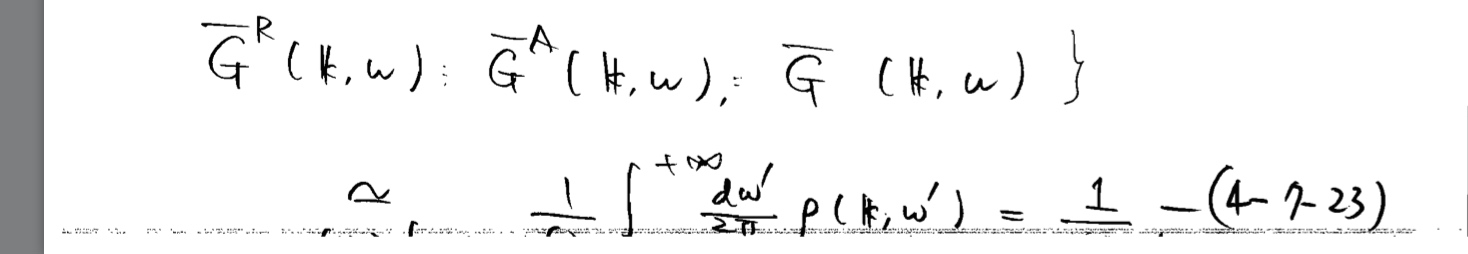
\includegraphics[width=\textwidth]{fig4-7-1.png}
\end{center}
%p757
\begin{center}
Analytic continuation from the temperature Green's functions to the real-time Green's functions.
\end{center}
 To see this, we again resort to the Lehmann representation of the Fourier coefficient of the temperature Green's function.
 According to eq.(\ref{4.4.13}), the Fourier coefficient is given by
\[
g(\mathbf{k},\omega_n)=\int_0^{\beta\hbar} d\tau e^{i\omega_n\tau} \int d^\mathbf{x} e^{-i\mathbf{k}\cdot \mathbf{x}} g(\mathbf{x},\tau;0,0)
\]
where we assume the spatial homogeneity.
%p758
\begin{equation}
\begin{aligned}
&=\int_0^{\beta\hbar} d\tau e^{i\omega_n\tau} \int d^\mathbf{x} e^{-i\mathbf{k}\cdot \mathbf{x}} \trace \left[ \hat \rho_G T_\tau \{ \psi_K(\mathbf{x},\tau) \psi_K^\dag (0,0) \} \right]\\
&=\int_0^{\beta\hbar} d\tau e^{i\omega_n\tau} \int d^\mathbf{x} e^{-i\mathbf{k}\cdot \mathbf{x}} \trace \left[ \hat \rho_G e^{-i\hat{\mathbf{P}}\cdot \mathbf{x}} e^{\hat K \tau/\hbar} \hat \psi (0) e^{-\hat K \tau/\hbar} e^{i\hat{\mathbf{P}}\cdot \mathbf{x}} \hat \psi^\dag (0) \right]\\
&=\int_0^{\beta\hbar} d\tau e^{i\omega_n\tau} \int d^\mathbf{x} e^{-i\mathbf{k}\cdot \mathbf{x}} \sum_{m,n} e^{\beta\Omega-\beta K_m} e^{-i(\mathbf{P}_m-\mathbf{P}_n)\cdot \mathbf x/\hbar} e^{(K_m-K_n)\tau/\hbar} |\langle m|\hat \psi (0)|n\rangle|^2\\
&=e^{\beta\Omega} \sum_{m,n} e^{-\beta K_m} \frac{1\mp e^{\beta(K_m-K_n)}}{i\omega_n-\hbar^{-1}(K_n-K_m)} (2\pi)^3 \delta^3(\mathbf k-\hbar^{-1}(\mathbf P_n -\mathbf P_m)) |\langle m|\hat \psi (0)|n\rangle|^2
\end{aligned}
\end{equation}
where
\[
\begin{aligned}
\omega_n&=\frac{2n\pi}{\beta\hbar} \qquad for \ boson\\
\omega_n&=\frac{(2n+1)\pi}{\beta\hbar} \qquad for \ fermion
\end{aligned}
\]
%p759
Comparing this with the definition of the spectral intensity, one can obtain
\begin{equation}
\begin{aligned}
g(\mathbf{k},\omega_n)&=e^{\beta\Omega} \sum_{m,n} (2\pi)^3 \delta^3(\mathbf k-\hbar^{-1}(\mathbf P_n -\mathbf P_m)) \frac{1}{i\omega_n-\hbar^{-1}(K_n-K_m)} \left( e^{-\beta K_m} \mp e^{-\beta K_n} \right) |\langle m|\hat \psi (0)|n\rangle|^2 \\
&=\int_{-\infty}^{+\infty} \frac{d\omega'}{2\pi} \frac{\rho(\mathbf k,\omega')}{i\omega_n-\omega'}
\end{aligned}
\end{equation}
an important relation between the spectral intensity and the temperature Green's function.
 This relation makes it possible to obtain the real-time Green's function from the temperature Green's function.
 More specifically, the perturbation analysis based on the Wick's theorem allows us to evaluate the temperature Green's function first.
%p760
 This means that the following function of 
\begin{equation}
\Gamma(\mathbf k,z)=\int _{-\infty}^{+\infty} \frac{d\omega'}{2\pi} \frac{\rho(\mathbf k,\omega)}{z-\omega'}
\end{equation}
a complex variable $z$ is known at the discrete set of points in the complex $z$-plane
\[
z=i\omega_n=
\left\{
\begin{aligned}
&\frac{2n\pi}{\beta\hbar}\qquad (boson)\\
&\frac{(2n+1)\pi}{\beta\hbar} \qquad (fermion)
\end{aligned}
\right.
\]
 Starting from these discretized points, we can perform an analytic continuation to the entire $z$-plane.
 Generally speaking, such an continuation cannot be performed in a unique way.
 For example, suppose that $\Gamma(\mathbf k,z)$ is one possible continuation.
%p761
 Then the function $\Gamma_p(\mathbf k,z)=\pm e^{p z \beta \hbar}\Gamma(\mathbf k,z)$ is also another possible continuation, because $\Gamma_p(\mathbf k,i\omega_n)=\Gamma(\mathbf k,i\omega_n)$ for an arbitrary odd integer $P$
\[
z=i\omega_n=
\left\{
\begin{aligned}
&\frac{2n\pi}{\beta\hbar}i\qquad (boson)\\
&\frac{(2n+1)\pi}{\beta\hbar}i \qquad (fermion)
\end{aligned}
\right.
\]
 However, the sum rule of the spectral intensity requires that the asymptotic behaviour of the analytic continuation in the large $\omega$ region should be always $\frac{1}{z}$.
\[
\lim_{|z|\to \infty} \Gamma(\mathbf k,z) \to \frac{1}{z} \int_{-\infty}^{+\infty} \frac{d\omega'}{2\pi} \rho(\mathbf k,\omega') =\frac{1}{z}
\]
which uniquely specify the appropriate analytic continuation out of these many possibilities.








\section{Linear response at finite temperature}
%p762
\begin{center}
linear response theory
\end{center}
 In this section, we will first introduce how to describe a linear response of the system against external perturbation at the finite temperature.
 The physical situations considered in the linear response theory is as follows.
 We first attach the system to the thermal bath at $t=-\infty$
\begin{center}
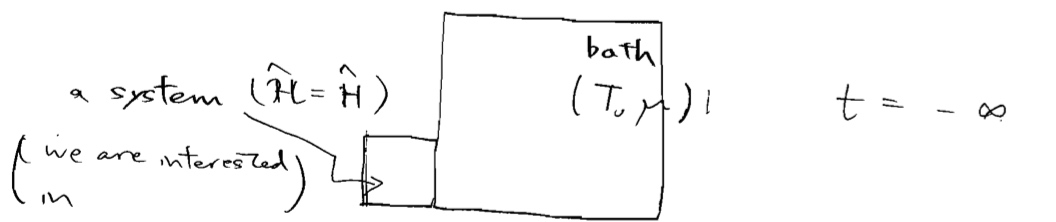
\includegraphics[width=0.8\textwidth]{fig4-8-1}
\end{center}
 Once the system is sufficiently equilibrated, we isolate the system from the bath.
%p763
\begin{center}
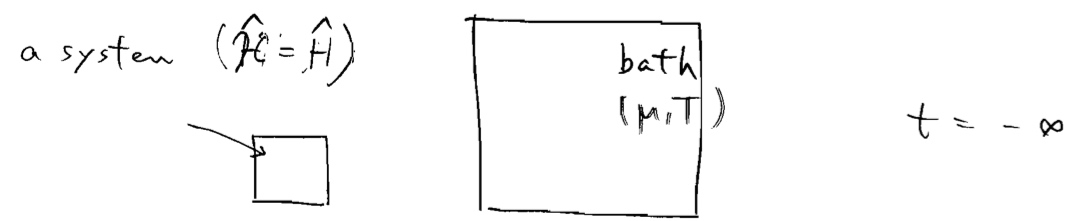
\includegraphics[width=0.8\textwidth]{fig4-8-2}
\end{center}
 Then, we adiabatically introduce an external perturbation $H^{ex}(t)$ since $t=-\infty$, where the system remains isolated from the bath.
\begin{center}
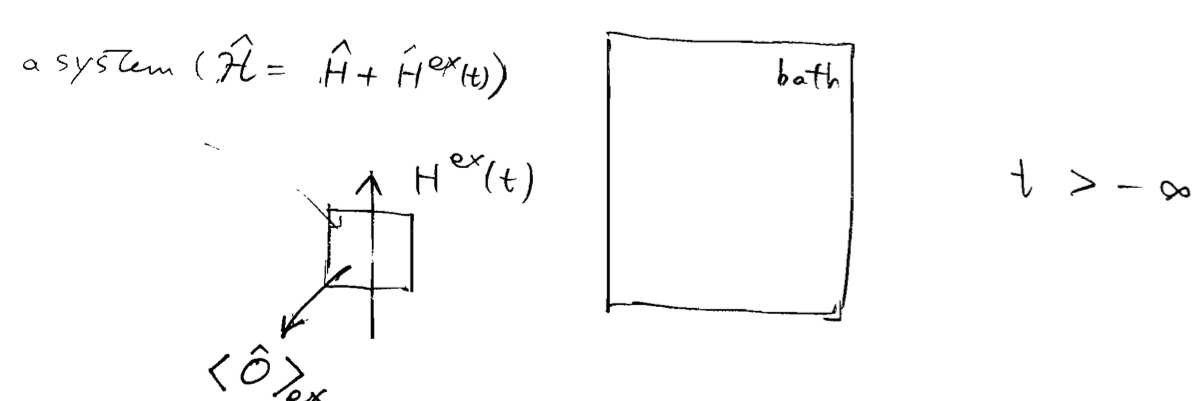
\includegraphics[width=0.8\textwidth]{fig4-8-3}
\end{center}
 At a given finite time t, we are going to measure a physical observable of the system within the first order in the external perturbation $H'(t)$
%p764
\begin{equation}\label{eq4.8.1}
\langle \hat O(t)\rangle_{ex}=e^{\beta\Omega} \sum_m e^{-\beta K_m} \langle m(t)|\hat O _s|m(t)\rangle
\end{equation}
 Such an observable is given in this way, where $\hat O_s$ is the operator for the observable in the Schrodinger picture.
 $|m(t)\rangle$ is an adiabatic evolution of an eigenstate $|m\rangle$ at $t=-\infty$
\[
\hat H |m\rangle=E_m|m\rangle
\]
\[
\hat N |m\rangle=N_m|m\rangle
\]
 These statistical weight is evaluated at $t=-\infty$, so that 
\[
K_m=E_m-N_m
\]
 The adiabatic time-evaluation of the eigenstate $| m\rangle$ is determined by $\hat H+\hat H^{ex}(t)$
%p765
\begin{equation}
i\hbar \frac{\partial}{\partial t}|m(t)\rangle=(\hat H+\hat H^{ex}(t))|m(t)\rangle
\end{equation}
 Within the linear order in $H'(t)$, the wavefunction at a finite time is given by
\begin{equation}
|m(t)\rangle=e^{-i\hat H t/\hbar}\left\{ |m\rangle -\frac{1}{\hbar} \int _{-\infty}^t dt' H_H^{ex}(t') |m\rangle+... \right\}
\end{equation}
where
\begin{equation}
H_H^{ex}(t) \equiv e^{i\hat Ht/\hbar} H^{ex} (t) e^{-\hat H t/\hbar}
\end{equation}
 Substituting this into eq.(\ref{eq4.8.1}), we have
\[
\langle \hat O(t)\rangle_{ex}=e^{\beta\Omega} \sum_m e^{-\beta K_m} \left\{ \langle m|\hat O_H(t)|m\rangle+\frac{i}{\hbar} \int_{-\infty}^t dt' \langle m|[\hat H_H^{ex}(t'),\hat O_H(t)]|m\rangle \right\}
\]
%p766
where the first term corresponds the observable without the external perturbation.
 Thus, the linear response of the observable is given by 
\[
\delta\langle\hat O(t)\rangle\equiv \langle O(t)\rangle_{ex}-\langle E(t)\rangle=\frac{i}{\hbar} \int_{-\infty}^t dt' \sum_m e^{-\beta K_m} \langle m|[\hat H_H^{ex}(t'),\hat O_H(t)]|m\rangle
\]
\begin{equation}\label{eq4.8.5}
\delta\langle\hat O(t)\rangle = \frac{i}{\hbar} \int_{-\infty}^t dt'\trace \left[ \hat \rho _G [\hat H_H^{ex}(t'),\hat O_H(t)]\right]
\end{equation}
\begin{center}
(electric) conductivities
\end{center}
 As an example of the linear response theory, let us consider the electric conductivity.
 Suppose that a system with charge-e particles is subjected under a spatially uniform electric field.
%p767
\begin{equation}
H^{ex}(t)=-\sum_i e(\hat{\mathbf{x}}\cdot \mathbf E) e^{-i\omega t}\equiv -\hat Ae^{-i\omega t}
\end{equation}
where $\hat {\mathbf{x}}_i$ denotes the spatial coordinate operator of $i$-th particle.
 We suppose that the applied electric field is time-dependent.
 In order to obtain the d.c. conductivity, we will take the frequency $\omega$ to be zero \uline{in the end of the calculation}
 Under the applied electric field, we are interested int he induced electric current density
\begin{equation}
\hat O\equiv \frac{1}{V} \frac{e}{m} \sum_j \hat{\mathbf{P}}_{j,v} \equiv \hat{\mathbf{J}}_V=\hat{\mathbf{j}}_V
\end{equation} 
where $\hat{\mathbf{P}}_g$ denotes the momentum operator of $j$-th particle.
%p768
 According to the linear response formula, which we sometimes call as Kubo formula, the induced current density at finite time ``t'' has the same time-dependence as the external electric field has
\begin{equation}
\begin{aligned}
\delta\langle\hat {\mathbf{j}_\nu}(t)\rangle&=- \frac{i}{\hbar} \int_{-\infty}^t dt'\trace \left[ \hat \rho _G [\hat A_H(t')e^{-i\omega t'},\hat {\mathbf{j}_{H,\nu}}(t)]\right]\\
&= \frac{i}{\hbar} \int_{-\infty}^t dt'e^{-i\omega t'} \left\{ \trace \left[ \hat \rho _G e^{i\hat H(t'-t)/\hbar} \hat A  e^{-i\hat H(t'-t)/\hbar} \hat{\mathbf j}_\nu \right] -\trace \left[ \hat \rho _G e^{i\hat H(t'-t)/\hbar} \hat {\mathbf{j}}_\nu  e^{-i\hat H(t'-t)/\hbar} \hat{A} \right] \right\}\\
&=e^{-i\omega t} \left(\frac{i}{\hbar} \right)\int_{-\infty}^t dt'e^{-i\omega( t'-t)}  \left\{ \trace \left[ \hat \rho _G e^{i\hat H(t'-t)/\hbar} \hat A  e^{-i\hat H(t'-t)/\hbar} \hat{\mathbf j}_\nu \right] -\trace \left[ \hat \rho _G e^{i\hat H(t'-t)/\hbar} \hat {\mathbf{j}}_\nu  e^{-i\hat H(t'-t)/\hbar} \hat{A} \right] \right\}\\
%p769
&=e^{-i\omega t} \left(\frac{i}{\hbar}\right) \int_{0}^{+\infty} dt' e^{i\omega t'} \trace \left[ \hat \rho _G [\hat A_H(t'),\hat {\mathbf{j}_{\nu}}]\right] \qquad (t'_{old}-t=-t'_{new})\\
&\overset{def}{\equiv} e^{-i\omega t} \mathbf j_\nu (\omega)
\end{aligned}
\end{equation}
\begin{equation}\label{eq4.8.9}
\left(
\begin{aligned}
\mathbf j_\nu (\omega)& = -\left(\frac{i}{\hbar}\right) \int_{0}^{+\infty} dt' e^{i\omega t'} \trace \left[ \hat \rho _G [\hat A_H(-t'),\hat {\mathbf{j}_{\nu}}]\right] \\
&\overset{def}{\equiv} \left(\frac{i}{\hbar}\right) \int_{0}^{+\infty} dt' e^{i\omega t'} X_\nu(t')
\end{aligned}
\right)
\end{equation}
 Now, the linear response coefficient $\mathbf j_\nu(\omega)$ is nothing but the (optical) conductivity.
 But, in order to calculate the correlation function between the position operator and the momentum operator
%p770
 On the one hand, the position operator (spatial coordinate operator) is ill-defined operator in the Hilbert space with periodic boundary condition.
 Consequently, it is formidable to treat in the momentum space representation, which we frequently use for its simplicity.
 In order to avoid treating the coordinate operators directly, we usually employ a following trick, so as to obtain conductivity.
 We first take a partial integral of the right hand side of eq.(\ref{eq4.8.9}).
%p771
\[
\begin{aligned}
\mathbf j_\nu (\omega)& \equiv \left(\frac{i}{\hbar}\right) \int_{0}^{+\infty} dt' e^{i\omega t'} X_\nu(t')\\
&=\left(\frac{i}{\hbar}\right) \int_{0}^{+\infty} dt' \frac{1}{i\omega} \frac{d e^{i\omega t'}}{dt'} X_\nu(t')\\
&=\left(\frac{i}{\hbar}\right)  \left[ \frac{1}{i\omega}  e^{i\omega t'} X_\nu(t')\right]_{t'=0}^{t'=+\infty}-\left(\frac{i}{\hbar}\right) \int_{0}^{+\infty} dt' \frac{1}{i\omega} e^{i\omega t'} \frac{d}{dt'} X_\nu(t')
\end{aligned}
\]
 Here we assume that $X_\mu(t)$ reduces to zero when $t$ goes to infinity $X_\nu(t=+\infty)=0$.
 This assumption is a plausible assumption, because $X_\nu(t=+\infty)$ is a correlation function between two quantities measured with an infinitely large \uline{time interval}.
%p772
With this assumption in mind, we have 
\begin{equation}\label{eq4.8.10}
\begin{aligned}
\mathbf j_\nu(\omega)&=\frac{i}{\hbar}\left[ -\frac{X_\nu(0)}{i\omega}-\int _0^{+\infty}  \frac{e^{i\omega t}}{i\omega} \frac{dX_\nu(t)}{dt} dt   \right]\\
&=-\frac{i}{\hbar} \int _0^{+\infty} \frac{e^{i\omega t }-1}{i\omega} \frac{dX_\nu(t)}{dt} dt  
\end{aligned}
\end{equation}
 Where
\[
X_\nu(t)\equiv - \trace\left[\hat \rho_G [\hat A_H(-t),\hat(\mathbf{j})_\nu]\right]
\]
 When it comes to $\frac{dX_\nu(t)}{t}$, we are free from the spatial coordinate operator.
 Namely, it is given by
\[
\frac{dX_\nu(t)}{dt}\equiv - \trace\left[\hat \rho_G [\frac{d\hat A_H(-t)}{dt},\hat(\mathbf{j})_\nu]\right]
\]
where
\[
\frac{d\hat A_H(-t)}{dt}=e^{-i \hat H t/\hbar}\frac{-i}{\hbar}[\hat  H,\sum_i \hat{\mathbf{x}}_i] e^{i \hat H t/\hbar} (e\mathbf E)
\]
where the temporal derivative of the spatial coordinate reduces to a current operator, latter of which is compatible with the periodic boundary condition
%p773
\begin{equation}
-\frac{i}{\hbar}[\hat  H,\sum_i \hat{\mathbf{x}}_i]=-\frac{e}{m}\sum_i\hat {\mathbf{p}}_i=-\hat{\mathbf{J}}
\end{equation}
 Namely, we have
\[
\frac{d\hat A_H(-t)}{dt}=-\hat{\mathbf{J}}_H(-t)\cdot \mathbf{E}
\]
and 
\begin{equation}
\begin{aligned}
\frac{dX_\nu(t)}{dt}&=\sum_\mu \trace \left[\hat \rho_G[\hat{\mathbf{J}}_{H,\mu}(-t),\hat{\mathbf j}_\nu]\right] \mathbf{E}_\mu\\
&=\frac{1}{V}\sum_\mu \trace \left[\hat \rho_G[\hat{\mathbf{J}}_{H,\mu}(-t),\hat{\mathbf J}_\nu]\right] \mathbf{E}_\mu\\
&=-\frac{1}{V}\sum_\mu \trace \left[\hat \rho_G[\hat{\mathbf{J}}_{H,\mu}(t),\hat{\mathbf J}_\nu]\right] \mathbf{E}_\mu
\end{aligned}
\end{equation}
%p774
Substituting this equation into eq.(\ref{eq4.8.10}), we finally obtain the induced current density within the linear order in the applied electric field.
\begin{equation}
\mathbf j_\nu(\omega)=\frac{i}{\hbar}\int_0^{+\infty} \frac{e^{i\omega t}-1}{\omega}\frac{1}{V} \sum_\mu \trace \left[ \hat \rho_G[\hat J_{H,\nu}(t),\hat J_{H,\mu}(0)] \mathbf E_\mu dt \right]
\end{equation}
\begin{equation}
\mathbf j_\nu (\omega)\overset{def}{\equiv} \sum_\mu \sigma_{\nu\mu}(\omega)\mathbf E_\mu
\end{equation}
where the conductivity is given by the retarded current-current correlation function.
\begin{equation}
\sigma_{\nu\mu}=-\frac{Q^R_{\nu\mu}(\omega)-Q^R_{\nu\mu}(0)}{i\omega}
\end{equation}
with
\begin{equation}
Q^R_{\nu\mu}(\omega)\equiv \int_{-\infty}^{+\infty} dt Q^R_{\nu\mu}(t)e^{i\omega t}
\end{equation}
%p775
 The retarded current-current correlation function is defined as follows
\begin{equation}
Q^R_{\nu\mu}(t)=-\frac{i}{\hbar V}\theta(t)\trace \left[ \hat \rho_G[\hat J_{H,\nu}(t),\hat J_{H,\mu}(0)] \right]
\end{equation}
 where $\hat J_{H,\mu}(t)=e^{i\hat Ht/\hbar} \hat J_\nu e^{-i\hat Ht/\hbar}$ and $\hat J_\nu$ is the $\nu$-th component of the total current.
 Contrary to the spatial coordinate operator, the current operator is well-defined operator in the Hilbert space with periodic boundary condition, so that, as for the conductivities, we usually apply this formula instead of eq.(\ref{eq4.8.5})
%p776
 As in the single-particle Green's function, the retarded current$^2$ correlation function has the corresponding temperature current$^2$ correlation function, latter of which allows us to use the perturbation theory based on Wick's theorem.
 Temperature current-current correlation function is defined as follows
\begin{equation}
\begin{aligned}
Q^T_{\nu\mu}(\tau,0)&=-\frac{1}{\hbar V} \trace \left[ \hat \rho_G T_\tau[\hat J_{K,\nu}(\tau),\hat J_{K,\mu}(0)] \right]\\
&=-\frac{1}{\hbar V}\left\{ \theta(\tau) \trace\left[ \hat \rho_G \hat J_{K,\nu}(\tau) \hat J_{K,\mu}(0) \right] + \theta(-\tau) \trace\left[ \hat \rho_G \hat J_{K,\mu}(0) \hat J_{K,\nu}(\tau) \right]\right\}
\end{aligned}
\end{equation}
where$\hat J_{K,\nu}(\tau)=e^{\hat{K}\tau/\hbar}\hat J_\nu e^{-\hat{K}_\tau/\hbar}$
and $\hat K=\hat H-\mu \hat N$
%p777
 Since the current operator commutes with total number of particle operator $[\hat J_\nu,\hat N]=0$, we can rewrite this as $\hat J_{K,\nu}=e^{\hat H\tau/\hbar}\hat J_\nu e^{-\hat H\tau/\hbar}$
 As in the single-particle Green's function, the Fourier series of this temperature correlation function is directly related to the Fourier transform of the retarded correlation function.
 The Fourier series of the temperature correlation function can be given by
\begin{equation}\label{eq4.8.19}
\begin{aligned}
Q^T_{\nu\mu}(i\omega_n)&=\int_0^{\beta\hbar} d\tau e^{i\omega_n \tau} Q^T_{\nu\mu}(\tau,0)\\
&=-\frac{1}{\hbar V} \int_0^{\beta\hbar} d\tau e^{i\omega_n \tau} e^{\beta\Omega} \sum_{m,n} e^{-\beta K_m} e^{(K_m-K_n)\tau/\hbar} \langle m|\hat J_\nu|n\rangle \langle n| \hat J_\mu|m\rangle\\
%p778
&=-\frac{1}{\hbar V} e^{\beta\Omega} \sum_{m,n} e^{-\beta K_m} \frac{e^{\beta(K_m-K_n)}-1}{i\omega_n-\hbar^{-1}(K_n-K_m)} \langle m|\hat J_\nu|n\rangle \langle n| \hat J_\mu|m\rangle\\
&=-\frac{1}{\hbar V} e^{\beta\Omega} \sum_{m,n} \frac{e^{-\beta K_n}-e^{-\beta K_m}}{i\omega_n-\hbar^{-1}(K_n-K_m)} \langle m|\hat J_\nu|n\rangle \langle n| \hat J_\mu|m\rangle\\
&\overset{def}{\equiv} \int_{-\infty}^{+\infty}\frac{d\omega'}{2\pi} \frac{\Delta_{J,\nu\mu}(\omega')}{i\omega_n-\omega'}
\end{aligned}
\end{equation}
where we define the spectral intensity for the current-current correlation function as follows
\begin{equation}
\Delta_{J,\nu\mu}(\omega)=-\frac{1}{\hbar V} e^{\beta\Omega} \sum_{m,n} \left( e^{-\beta K_n}-e^{-\beta K_m} \right) 2\pi \delta(\omega-\hbar^{-1}(K_n-K_m)) \langle m|\hat J_\nu|n\rangle \langle n| \hat J_\mu|m\rangle
\end{equation}
%p779
 On the one hand, retarded current-current correlation function can be given by the following Lehmann representation.
\begin{equation}
Q^R_{\nu\mu}(t)=-\frac{i}{\hbar V} \theta(t) \left\{ \trace[\hat \rho_G e^{i\cancelto{\hat K}{\hat Ht/\hbar}} \hat J_\nu e^{-i\cancelto{\hat K}{\hat Ht/\hbar}} \hat J_\mu]- \trace[\hat \rho_G \hat J_\mu e^{i\cancelto{\hat K}{\hat Ht/\hbar}} \hat J_\nu e^{-i\cancelto{\hat K}{\hat Ht/\hbar}} ] \right\}
\end{equation}
Since the current operator commutes with the total number of particle operator $\hat N$: $[\hat J_\nu,\hat N]=0$, we can rewrite this as 
\[
e^{i\hat Ht/\hbar} \hat J_\nu e^{-i\hat Ht/\hbar} =e^{i\hat Kt/\hbar} \hat J_\nu e^{-i\hat Kt/\hbar} 
\]
with 
\[
\begin{aligned}
\hat K&=\hat H-\mu \hat N\\
&=-\frac{i}{\hbar V} \theta(t)e^{\beta\Omega} \sum_{m,n}\left( e^{-\beta K_m} e^{i(K_m-K_n)t/\hbar}-e^{-\beta K_n} e^{i(K_m-K_n)t/\hbar} \right)  \langle m|\hat J_\nu|n\rangle \langle n| \hat J_\mu|m\rangle
\end{aligned}
\]
%p780
Accordingly, the Fourier transformation of the retarded correlation function can be calculated as follows:
\begin{equation}\label{eq4.8.22}
\begin{aligned}
Q^R_{\nu\mu}(\omega)&=\int_{-\infty}^{+\infty} dte^{i\omega t} Q^R_{\nu\mu}(t)\\
&=\frac{1}{\hbar V}e^{\beta\Omega} \sum_{m,n} \frac{e^{-\beta K_m}-e^{-\beta K_n}}{\omega-\hbar^{-1}(K_n-K_m)+i\eta} \langle m|\hat J_\nu|n\rangle \langle n| \hat J_\mu|m\rangle\\
&=\int_{-\infty}^{+\infty} \frac{d\omega'}{2\pi} \frac{\Delta_{J,\nu\mu}(\omega')}{\omega-\omega'+i\eta}
\end{aligned}
\end{equation}
 Thus, the comparison between eq.(\ref{eq4.8.19}), eq.(\ref{eq4.8.22}) suggests that the Fourier series of the retarded correlation function can be obtained from that of the temperature correlation function by the analytic continuation.
%p781
\begin{equation}
Q^R_{\nu\mu} (\omega)=Q^T_{\nu\mu}(i\omega_n=\omega+i\eta)
\end{equation}
where the conductivity is given by
\begin{equation}
\sigma_{\nu\mu}(\omega)=-\frac{Q^R_{\nu\mu}(\omega)-Q^R_{\nu\mu}(0)}{i\omega}
\end{equation}
 In practice, we first calculate the temperature current-current correlation function by using perturbation expansion based on the Wick's theorem.
 Then, we obtain the corresponding retarded current-current correlation function by this relation, from which we obtain the conductivity of the many-particle systems.\\
%782
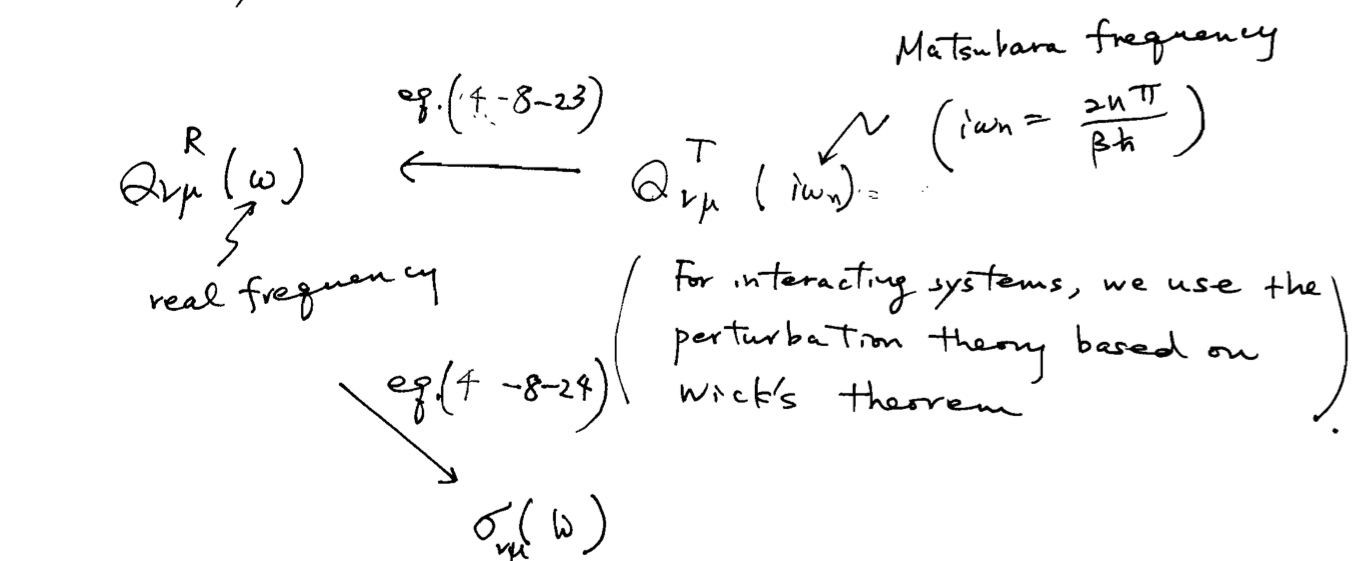
\includegraphics[width=\textwidth]{fig4-8-4}
%783
 As the second example of the linear response theory at finite temperature, let us next consider the ``screening effect'' and ``plasma oscillation'' in the degenerate electron gas at finite temperature.










\section{Screening effect \& plasma oscillation in an electron gas at finite (or high) temperature}
 As in sec.(\_), we suppose that an electron gas is subjected under an applied scalar potential.
\begin{equation}
\hat H^{ex}_H(t)=-\int d^3\mathbf x \hat n_H(\mathbf x,t) e\phi^{ex}(\mathbf x,t)
\end{equation}
with $\hat n_H(\mathbf x ,t)=e^{i \hat H t/\hbar} \hat n(\mathbf x)e^{-i \hat Ht/\hbar}$
\begin{equation}
[\hat n(\mathbf x),\hat N]=e^{i \hat K t/\hbar} \hat n(\mathbf x)e^{-i \hat Kt/\hbar}
\end{equation}
%p784
According to eq.( ), the induced density is given by the retarded density-density correlation function.
\begin{equation}
\begin{aligned}
\delta\langle n(\mathbf x,t)\rangle &=\frac{i}{\hbar} \int_{-\infty}^t dt' \trace\left[ \hat \rho_G[\hat H^{ex}_H(\mathbf x',t'),\hat n_H(\mathbf x,t)] \right]\\
&=-\frac{i}{\hbar}\int d^3 \mathbf x' \int_{-\infty}^t dt' \trace\left[ \hat \rho_G[\hat n_H(\mathbf x',t'),\hat n_H(\mathbf x,t)] \right] e\phi^{ex}(\mathbf x',t')\\
&=-\frac{1}{\hbar} \int d^3 \mathbf x' \int_{-\infty}^t dt' D^R(\mathbf x,t;\mathbf x',t')e\phi^{ex}(\mathbf x',t')
\end{aligned}
\end{equation}
where the retarded correlation function is defined as follows
\[
iD^R(\mathbf x,t;\mathbf x',t')=\theta(t-t')\trace\left[ \hat \rho_G[\hat n_H(\mathbf x',t'),\hat n_H(\mathbf x,t)] \right]
\]
Since this bracket is the commutator, we can replace these density operators by the density derivative operators. (I guess this word is ``operators'' -- Peng Pai)
%p785
\begin{equation}
=\theta(t-t')\trace \left[ \hat \rho_G[\delta \hat n_H(\mathbf x',t'),\delta \hat n_H(\mathbf x,t)] \right]
\end{equation}
with $\delta \hat n_H(\mathbf x,t)\equiv e^{i\hat K t/\hbar}\delta \hat n(\mathbf x)e^{-i\hat Kt/\hbar}$ and
\begin{equation}\tag{4.9.4'}
\delta \hat n(\mathbf x)=\hat n(\mathbf x)-\langle \hat n(\mathbf x)\rangle
\end{equation}
 The corresponding temperature function is given by 
\begin{equation}
D^T(\mathbf x,t;\mathbf x',t')=-\trace\left[ \hat \rho_GT_\tau[\delta \hat n_H(\mathbf x',t')\delta\hat n_H(\mathbf x,t)] \right]
\end{equation}
 The Fourier series of these two functions are related to each other by the spectral intensity
\begin{equation}
\begin{aligned}
D^T(\mathbf k,i\omega_n)&=\int d^3(\mathbf x-\mathbf x')\int _0^{\beta\hbar}d(\tau-\tau')e^{-i\mathbf k\cdot(\mathbf x-\mathbf x')}e^{i\omega_n (\tau-\tau')}D^T(\mathbf x,t;\mathbf x',t')\\
&=-\int d^3(\mathbf x-\mathbf x')\int _0^{\beta\hbar}d(\tau-\tau')e^{-i\mathbf k\cdot(\mathbf x-\mathbf x')}e^{i\omega_n (\tau-\tau')} e^{\beta\Omega} \sum_{m,n} e^{-\beta K_m}\\
&\quad\langle m|e^{-i\mathbf P\cdot \mathbf x/\hbar} e^{\hat K \tau/\hbar} \delta \hat n(\mathbf 0) e^{-\hat K \tau/\hbar} e^{i\mathbf P\cdot \mathbf x/\hbar} |n\rangle \langle m|e^{-i\mathbf P\cdot \mathbf x'/\hbar} e^{\hat K \tau'/\hbar} \delta \hat n(\mathbf 0) e^{-\hat K \tau'/\hbar} e^{i\mathbf P\cdot \mathbf x'/\hbar} |n\rangle\\ 
%p786
&=-\int d^3(\mathbf x-\mathbf x')\int _0^{\beta\hbar}d(\tau-\tau')e^{-i\mathbf k\cdot(\mathbf x-\mathbf x')}e^{i\omega_n (\tau-\tau')} e^{\beta\Omega} \sum_{m,n}e^{-\beta K_m}\\
&\quad e^{-i(\mathbf P_m-\mathbf P_n)\cdot(\mathbf x-\mathbf x')/\hbar} e^{(K_m-K_n)(\tau-\tau')/\hbar} |\langle m|\delta\hat n(0)|n\rangle|^2\\
&=-e^{\beta\Omega} \sum_{m,n} e^{-\beta K_m} (2\pi)^3 \delta^3(\mathbf k-\hbar^{-1}(\mathbf P_n-\mathbf P_m))\frac{e^{(K_m-K_n)\beta}-1}{i\omega_n-\hbar^{-1}(K_n-K_m)}|\langle m|\delta \hat n(0)|n\rangle|^2\\
&=\int_{-\infty}^{\infty}\frac{d\omega'}{2\pi}\frac{\Delta(\mathbf k,\omega')}{i\omega_n-\omega'}
\end{aligned}
\end{equation}

\begin{equation}
\begin{aligned}
D^R(\mathbf k,\omega)&=\int d^3(\mathbf x-\mathbf x')\int _0^{\beta\hbar}d(t-t')e^{-i\mathbf k\cdot(\mathbf x-\mathbf x')}e^{i\omega (t-t')}D^R(\mathbf x,t;\mathbf x',t')\\
&=-\int d^3(\mathbf x-\mathbf x')\int _0^{\beta\hbar}d(t-t')e^{-i\mathbf k\cdot(\mathbf x-\mathbf x')}e^{i\omega (t-t')}\\
&\quad (-i)\Big\{ \theta(t-t') e^{\beta\Omega} \sum_{m,n}e^{-i\beta K_m} e^{-i(\mathbf P_m-\mathbf P_n)\cdot(\mathbf x-\mathbf x')/\hbar} e^{i(K_m-K_n)(t-t')/\hbar} |\langle m|\delta\hat n(0)|n\rangle|^2\\
& \quad-\theta(t-t') e^{\beta\Omega} \sum_{m,n}e^{-i\beta K_n} e^{-i(\mathbf P_m-\mathbf P_n)\cdot(\mathbf x-\mathbf x')/\hbar} e^{i(K_m-K_n)(t-t')/\hbar} |\langle m|\delta\hat n(0)|n\rangle|^2\Big\}\\
%p787
&=e^{\beta\Omega} \sum_{m,n}\left\{ e^{-\beta K_m} (2\pi)^3 \delta^3(\mathbf k-\hbar^{-1}(\mathbf P_n-\mathbf P_m))\frac{1}{\omega-\hbar^{-1}(K_n-K_m)+i\eta}|\langle m|\delta \hat n(0)|n\rangle|^2\right\}\\
&=\int_{-\infty}^{\infty}\frac{d\omega'}{2\pi}\frac{\Delta(\mathbf k,\omega')}{\omega-\omega'+i\eta}
\end{aligned}
\end{equation}
where
\begin{equation}
\Delta(\mathbf k,\omega)=e^{\beta\Omega}\sum_{m,n} (2\pi)^3 \delta^3(\mathbf k-\hbar^{-1}(\mathbf P_n-\mathbf P_m)) 2\pi\delta(\omega-\hbar^{-1}(K_n-K_m))(e^{-\beta K_m}-e^{-\beta K_n}) |\langle m|\delta \hat n(0)|n\rangle|^2
\end{equation}
 These two Lehmann representations concludes that the Fourier series of the retarded function can be contained by the Fourier series of the temperature function.
%792
\begin{equation}\label{eq4.9.9}
D^R(\mathbf k,\omega)=D^T(\mathbf k,i\omega_n=\omega+i\eta)
\end{equation}
 In terms of the retarded density-density correlation function, the density deviation induced by the external scalar potential is given by
\begin{equation}\label{eq4.9.10}
\begin{aligned}
\langle \delta n(\mathbf x,t)\rangle &=\int \frac{d^3\mathbf k}{(2\pi)^3}\int \frac{d\omega}{2\pi} e^{i\mathbf k\cdot \mathbf x}e^{-i\omega t}\langle \delta n(\mathbf k,\omega)\rangle\\
\phi ^{ex}(\mathbf x,t)&=\int \frac{d^3\mathbf k}{(2\pi)^3}\int \frac{d\omega}{2\pi} e^{i\mathbf k\cdot \mathbf x}e^{-i\omega t} \phi ^{ex}(\mathbf k,\omega)\\
\langle \delta n(\mathbf k,\omega)\rangle&=-\frac{e}{\hbar}D^R(\mathbf k,\omega)\phi^{ex}(\mathbf k,\omega)
\end{aligned}
\end{equation}
 In order to calculate the retarded function, we will calculate the temperature function, and use this formula.
 The temperature density-density correlation function can be calculated in terms of the perturbation theory based on the Wick's theorem.
%p793
\[
\begin{aligned}
D^T(\mathbf x,\tau;\mathbf x',\tau')&=-e^{\beta\Omega}\trace[e^{-\beta \hat K}T_\tau\{ \delta \hat n_k(\mathbf x ,\tau)\delta \hat n_k(\mathbf x' ,\tau') \}]\\
&=-\left\{e^{\beta\Omega}\trace[e^{-\beta \hat K}T_\tau\{ \hat n_k(\mathbf x ,\tau)\hat n_k(\mathbf x' ,\tau') \}] -\langle \hat n(\mathbf x)\rangle \langle \hat n (\mathbf x')\rangle \right\}\\
&=-\left\{e^{\beta\Omega}\trace[e^{-\beta \hat K}T_\tau\{ \psi_K^\dag(\mathbf x,\tau)\psi_K(\mathbf x,\tau) \psi_K^\dag(\mathbf x',\tau')\psi_K(\mathbf x',\tau') \}] -\langle \hat n(\mathbf x)\rangle \langle \hat n (\mathbf x')\rangle \right\}
\end{aligned}
\]
As we did in sec.2-8 (for the zero-temperature field theory), let us first introduce two-particle temperature Green's function at the finite temperature.
\begin{equation}
g(\mathbf x_1,\tau_1;\mathbf x_2,\tau_2;\mathbf x_1',\tau_1';\mathbf x_2',\tau_2')=\trace [\hat \rho_G T_\tau\{\psi_K(\mathbf x_1,\tau_1)\psi_K(\mathbf x_2,\tau_2)\psi_K^\dag(\mathbf x_2',\tau_2')\psi_K^\dag(\mathbf x_1',\tau_1')\}]
\end{equation}
where
\[
\begin{aligned}
\hat \psi_K(\mathbf x ,\tau)&=e^{\hat K\tau/\hbar}\hat \psi(\mathbf x)e^{-\hat K\tau/\hbar}\\
\hat \psi_K(\mathbf x' ,\tau')&=e^{\hat K\tau'/\hbar}\hat \psi(\mathbf x')e^{-\hat K\tau'/\hbar}\\
\end{aligned}
\]
with $\hat K=\hat H-\mu \hat N$ (I can't see that clearly--Peng Pai)
%p794
 In order to apply the perturbation theory to the two-particle temperature Green's function, we again rewrite this interns of the interaction picture.
 We can do this exactly in the asme way as we did for the single-particle temperature Green's function
\[
g(\mathbf x_a,\tau_a;\mathbf x_b,\tau_b;\mathbf x_a',\tau_a';\mathbf x_b',\tau_b')=\frac{numerator}{denominator}
\]
\[
\begin{aligned}
(numerator)&=\trace [ \cancelto{\rho^0_G=e^{\beta\Omega_0-\beta\hat K_0}}{e^{-\beta\hat K_0}}\qquad \qquad\qquad\qquad\sum_{\nu=0}^{+\infty}\left( -\frac{1}{\hbar}\right)^\nu \frac{1}{\nu!}\int_0^{\beta}d\tau_1 ... \int_0^{\beta}d\tau_\nu\\
 &\quad T_\tau\{ \hat H_1(\tau_1)...\hat H_1(\tau_\nu) \hat\psi_I(\mathbf x_a,\tau_a) \psi_I(\mathbf x_b,\tau_b) \psi_I^\dag(\mathbf x_b',\tau_b') \psi_I^\dag(\mathbf x_a',\tau_a') \}  ]
\end{aligned}
\]
\begin{equation}
(denominator)=\trace [ \cancelto{\rho^0_G}{e^{-\beta\hat K_0}}\qquad\sum_{\nu=0}^{+\infty}\left( -\frac{1}{\hbar}\right)^\nu \frac{1}{\nu!}\int_0^{\beta}d\tau_1 ... \int_0^{\beta}d\tau_\nu\quad T_\tau\{ \hat H_1(\tau_1)...\hat H_1(\tau_\nu)  \}  ]
\end{equation}
with 
\[
\left.
\begin{aligned}
\hat\psi_I(\mathbf x,\tau)&=e^{\hat K_0\tau/\hbar} \hat \psi(\mathbf x)e^{-\hat K_0\tau/\hbar}\\
\hat\psi_I^\dag(\mathbf x,\tau)&=e^{\hat K_0\tau/\hbar} \hat \psi^\dag(\mathbf x)e^{-\hat K_0\tau/\hbar}
\end{aligned}
\right\}
\]
%p795
\begin{equation}
\hat H_1(\tau)\equiv e^{\hat K_0\tau/\hbar}\hat H_1e^{-\hat K_0\tau/\hbar}
\end{equation}
 For each of these two, we can employ the Wick theorem, which contracts creation field and annihilation field.
 As in the case of the single-particle temperature Green's function, we end up with a sum of all possible fully-contracted terms.
 Each of these fully-contracted terms can be described by a Feynman diagram.
 Let us first consider the numerator.
 now that we have four external fermion fields within the reach of the numerator, the Feynman diagram obtained from the numerator has four external points
%p796
which are specified by these four coordinate variables.\\
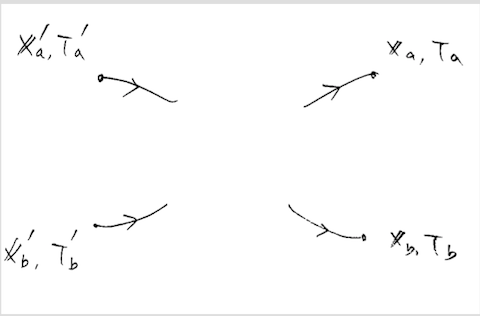
\includegraphics[width=0.5\textwidth]{fig4-9-1}\\
 For example, for the second order in the interaction potential, we have following two Feynman diagrams.\\
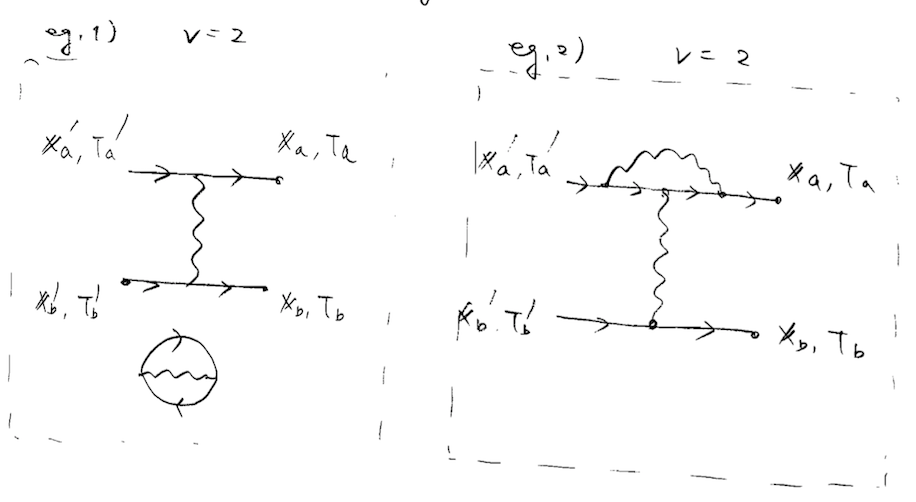
\includegraphics[width=\textwidth]{fig4-9-2}\\
Since the one of the two interaction potential 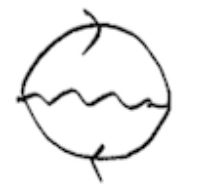
\includegraphics[width=1cm]{fig4-9-3} is disconnected from these four external points, we call this type of diagram
%p797
as non-connected Feynman diagram.
 On the one hand, both of these two interaction lines are connected to the external points in this diagram, we call the latter type of diagram as the connected Feynman diagram.
 As we proved for the single-particle temperature Green's functions, all the non-connected Feynman diagrams in the numerator are canceled by the denominator.
 As a result, two-particle temperature Green's function is given by a sum of all possible connected Feynman diagram.
%p798
\begin{equation}
\begin{aligned}
g(\mathbf x_a,\tau_a;\mathbf x_b,\tau_b;\mathbf x_a',\tau_a';\mathbf x_b',\tau_b')&=\trace [ \rho^0_G \sum_{\nu=0}^{+\infty}\left( -\frac{1}{\hbar}\right)^\nu \frac{1}{\nu!}\int_0^{\beta}d\tau_1 ... \int_0^{\beta}d\tau_\nu\\
&\quad  T_\tau\{ \hat H_1(\tau_1)...\hat H_1(\tau_\nu) \hat\psi_I(\mathbf x_a,\tau_a) \psi_I(\mathbf x_b,\tau_b) \psi_I^\dag(\mathbf x_b',\tau_b') \psi_I^\dag(\mathbf x_a',\tau_a') \}  ]
\end{aligned}
\end{equation}
 Feynman's rule for the two-particle temperature Green's function can be easily derived as the generalisation of that for the single-particle temperature Green's function.
 For $n$-th order contribution,\\
(a) Draw all topologically district connected Feynman diagram with the four external; points, which are composed of $n$-interaction line (wavy line) and ($2n+2$) non-interacting temperature Green's function $g^0$ (directed solid lines)\\
(b) Associate a factor $g^0(1,2)$ with each directed solid line running from $2$ to $1$.\\
%p799
(c) Associate a factor $V_0(1,2)=V_0(\mathbf x_1-\mathbf x_2)\delta(\tau_1-\tau_2)$ with each wavy line joining $1$ and $2$.\\
(d) Integrate all the internal variables $\int d^3\mathbf x_i\int_0^{\beta\hbar}d\tau_i$\\
(e) Multiply each $n$-th order diagram by $(-1/\hbar)^n(-1)^F$. $F$ is the number of the closed loops formed by directed solid lines when the external point $\mathbf x_a,\tau_a$ is connected to $\mathbf x_a',\tau_a'$ by a sequence of the solid lines.
%p800
When the external point $\mathbf x_a,\tau_a$ is connected to $\mathbf x_b',\tau_b'$, (F+1) is the number of the closed loops.\\
(f) Interpret any temperature Green's function at equal time variable as follows 
\[
g^0(\mathbf x_i,\tau_i;\mathbf x_j,\tau_i)=\lim_{\tau_j\to \tau_i+\eta}g^0(\mathbf x_i,\tau_i;\mathbf x_j,\tau_j)
\]
\rule{\textwidth}{0.1mm}
With this Feynman rule in mind, let us go back to the evaluation of the temperature density-density correlation function.
\begin{equation}
D^T(\mathbf x,\tau;\mathbf x',\tau')=-\{ g(\mathbf x,\tau;\mathbf x',\tau';\mathbf x,\tau+;\mathbf x',\tau'+)-g(\mathbf x,\tau;\mathbf x,\tau+)g(\mathbf x',\tau';\mathbf x',\tau'+) \}
\end{equation}
%p801
 Where this temperature Green's function denotes the two-particle Green's function introduced so far.
 These two temperature Green's function stand for the single-particle one, which correspond to these mean density
\begin{equation}
g(\mathbf x,\tau;\mathbf x,\tau+)=-\trace[\hat \rho_G\hat \psi^\dag(\mathbf x)\hat \psi(\mathbf x)]=-\langle \hat n(\mathbf x)\rangle
\end{equation}
 As we described so far, the two-particle temperature Green's function is given by a sum of all possible connected Feynman diagrams with the four external points.\\
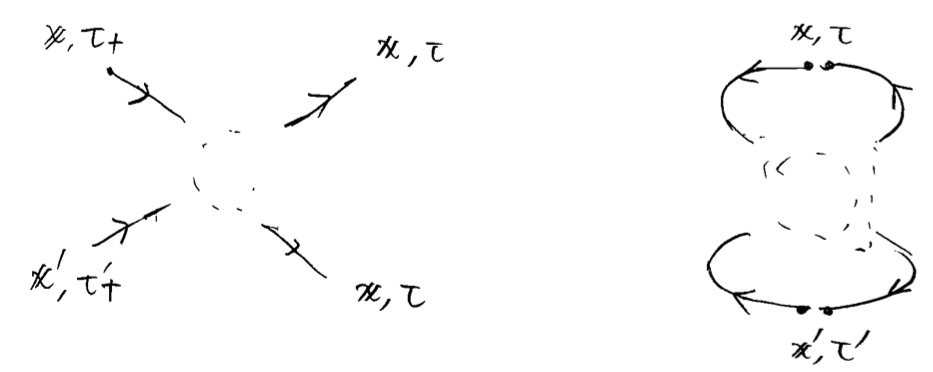
\includegraphics[width=0.8\textwidth]{fig4-9-4}
%p802
 Since these two external points and these two external points coincide respectively, we draw this diagram like this.
 Generally, such connected diagrams consist of two types of diagram.
 In the first type, the external line emitting from $\mathbf x,\tau$ and that from $\mathbf x',\tau'$ are disconnected\\
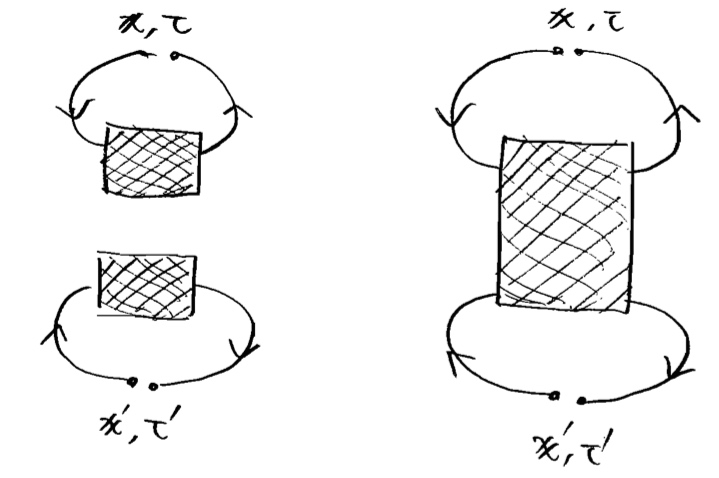
\includegraphics[width=0.5\textwidth]{fig4-9-5}
 In the other type, these two external lines are connected by either solid lines or wavy lines (interaction lines)
%p803
 As we have discussed in sec 2.8 in the context of the zero-temperature field theory, the former types of diagrams are given by the product between two single-particle Green's functions, which are cancelled by the second term in this bracket.
 As a result, the temperature density$^2$ correlation function is given by a sum of all possible connected Feynman diagrams in which these two external lines are connected.
\begin{equation}
D^T(\mathbf x,\tau;\mathbf x',\tau')=-g^{\uline{(c)}}(\mathbf x,\tau;\mathbf x',\tau';\mathbf x,\tau+;\mathbf x',\tau'+)
\end{equation}
where this (c) means that the upper external line and (I can't see clearly -- Peng Pai)\\
%p804
As in the zero-temperature field theory, we can derive a Dyson equation for such temperature correlation function.
\begin{equation}
\begin{aligned}
-D^{T}(\mathbf x,\tau;\mathbf x',\tau')=&-D^{T,\star}(\mathbf x,\tau;\mathbf x',\tau')\\
&+\int d^3\mathbf x_1 \int_0^{\beta\hbar}d\tau_1\int d^3\mathbf x_2\int _0^{\beta\hbar}(-D^{T,\star}(\mathbf x,\tau;\mathbf x_1,\tau_1)\\
&\left(-\frac{1}{\hbar}\right)V_0(\mathbf x_1-\mathbf x_2)\delta(\tau_1-\tau_2)\left(-D^T(\mathbf x_2,\tau_2;\mathbf x',\tau')\right)
\end{aligned}
\end{equation}
where $D^{T,\star}$ corresponds to a proper part of the density-density correlation, which cannot be decomposed into two parts by cutting a single interaction line.
 In terms of the Feynman diagram, this equation can be schematically drawn like this.\\
%p805
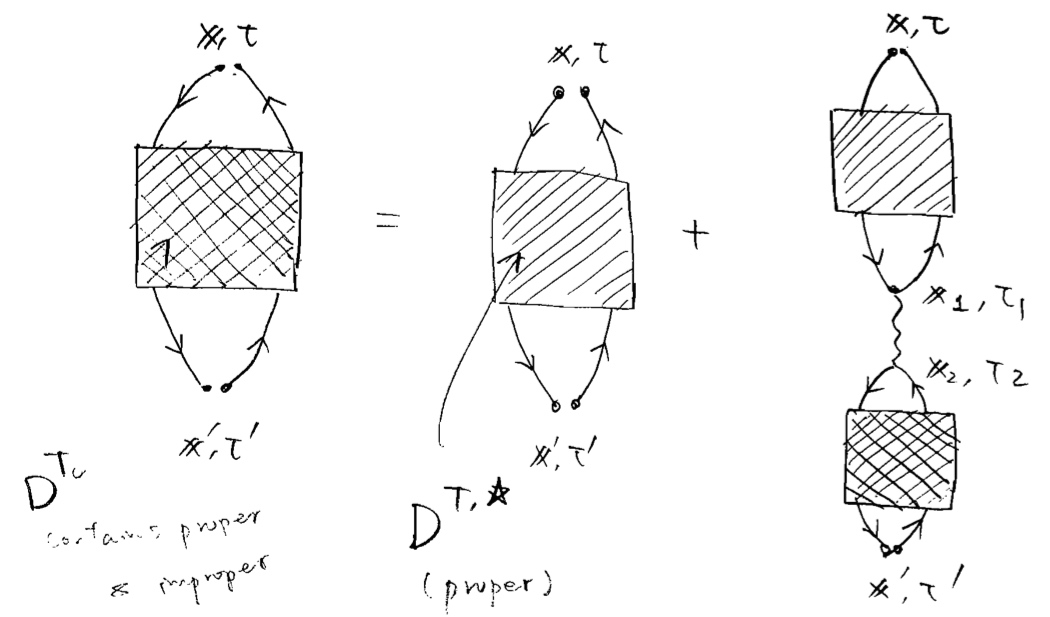
\includegraphics[width=0.8\textwidth]{fig4-9-6}
 In order to set off this plank constant, we again define the ``temperature version'' of the polarisation part as
\begin{equation}
\Pi^T(\mathbf x,\tau;\mathbf x',\tau')=\frac{1}{\hbar}D^T(\mathbf x,\tau;\mathbf x',\tau')
\end{equation} 
 In terms of this, the Dyson equation becomes as follows.
\begin{equation}
\begin{aligned}
\Pi^{T}(\mathbf x,\tau;\mathbf x',\tau')=&\Pi^{T,\star}(\mathbf x,\tau;\mathbf x',\tau')\\
&+\int d^3\mathbf x_1 \int_0^{\beta\hbar}d\tau_1\int d^3\mathbf x_2\int _0^{\beta\hbar}(\Pi^{T,\star}(\mathbf x,\tau;\mathbf x_1,\tau_1)\\
&V_0(\mathbf x_1-\mathbf x_2)\delta(\tau_1-\tau_2)\Pi^T(\mathbf x_2,\tau_2;\mathbf x',\tau')
\end{aligned}
\end{equation}
%p806
 Or equivalently
\begin{equation}
\Pi^T(\mathbf k,i\omega_n)=\Pi^{T,\star}(\mathbf k,i\omega_n)+\Pi^{T,\star}(\mathbf k,i\omega_n)V_0(\mathbf k)\Pi^T(\mathbf k,i\omega_n)
\end{equation}
 where we assume the spatial homogeneity
\begin{equation}
\Pi^{T,(\star)}(\mathbf k,i\omega_n)\overset{def}{\equiv}\int d^3(\mathbf x-\mathbf x')\int_0^{\beta\hbar} d(\tau-\tau') e^{-i\mathbf k\cdot(\mathbf x-\mathbf x')} e^{i\omega_n(\tau-\tau')} \Pi^{T,(\star)}(\mathbf x,\tau;\mathbf x',\tau')
\end{equation}
 This algebraic equation can be easily solved in terms of the proper part
\begin{equation}
\Pi^T(\mathbf k,i\omega_n)=\frac{\Pi^{T,\star}(\mathbf k,i\omega_n)}{1-\Pi^{T,\star}(\mathbf k,i\omega)V_0(\mathbf k)}
\end{equation}
 Accordingly, using eq.(\ref{eq4.9.9}), we finally obtain the retarded density-density correlation function in terms of the proper polarisation part.
%p807
\begin{equation}
\begin{aligned}
D^R(\mathbf k,\omega)&=D^T(\mathbf k,i\omega_n=\omega+i\eta)\\
&=\hbar \Pi^T(\mathbf k,i\omega_n=\omega+i\eta)\\
&=\frac{\hbar \Pi^{T,\star}(\mathbf k,i\omega_n=\omega+i\eta)}{1-\Pi^{T,\star}(\mathbf k,i\omega_n=\omega+i\eta)V_0(\mathbf k)}
\end{aligned}
\end{equation}
In order to evaluate the proper polarisation part, we need a certain approximation in general.\\
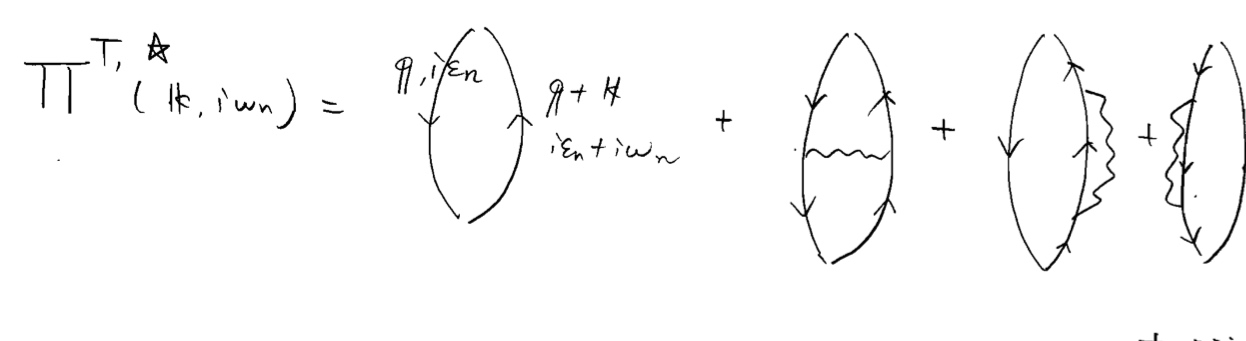
\includegraphics[width=\textwidth]{fig4-9-7}\\
As the most primitive approximation, let us retain the lowest order contribution to the proper polarisation part.
\begin{equation}\label{eq4.9.24}
\Pi^{T,\star}(\mathbf k,i\omega_n)\approx \Pi^{T,0}(\mathbf k,i\omega_n)
\end{equation}
%p808
\begin{equation}
-\hbar \Pi^{T,0}(\mathbf k,i\omega)=-\frac{1}{\beta\hbar} \sum_{i\epsilon_n} \int \frac{d^3 \mathbf q}{(2\pi)^3} g^0(\mathbf q,i\epsilon_n) g^0(\mathbf k+\mathbf q,i\omega_n+i\epsilon_n)
\end{equation}
where this ``-'' sign comes from this or comes from the exchange between these two fermion fields.
\begin{equation}
\Pi^{T,0}(\mathbf k,i\omega)\not=\frac{\cancel{2}{1}}{\beta\hbar^2} \sum_{i\epsilon_n} \int \frac{d^3\mathbf q}{(2\pi)^3}\frac{1}{i\omega_n+i\epsilon_n-\hbar^{-1}(\epsilon^0_{\mathbf k+\mathbf q}-\mu)} \frac{1}{i\epsilon_n-\hbar^{-1}(\epsilon^0_{\mathbf q}-\mu)}
\end{equation}
 So far, we have omitted the spin index, assuming the spin rotational symmetry.
 If we take into account the son degree of freedom, we need to add a factor $(2s+1)$ which comes from the summation over
%p809
the spin index along this closed loop.
 For spin-$1/2$ electron, we thus put a factor 2.
 Since this particle line is for the fermion, the summation over the Matsubara frequency is taken over $i\epsilon_n=\frac{(2n+1)\pi}{\beta\hbar}$
 Such a summation can be evaluated in terms of the complex integral, as we did in sec. 4-4.
\begin{equation}
\begin{aligned}
\Pi^{T,0}(\mathbf k,i\omega_n)&=\frac{2}{\hbar}\int \frac{d^3 \mathbf q}{(2\pi)^3} \int\frac{dz}{2\pi i}\frac{1}{e^{\beta\hbar z}+1} \frac{1}{z+i\epsilon_n-\hbar^{-1}(\epsilon^0_{\mathbf k+\mathbf q}-\mu)} \frac{1}{z-\hbar^{-1}(\epsilon^0_{\mathbf q}-\mu)}\\
&=\frac{2}{\hbar} \int \frac{d^3\mathbf q}{(2\pi)^3} \frac{n^0_{\mathbf k+\mathbf q}-n^0_{\mathbf q}}{-i\omega_n+\hbar^{-1}(\epsilon^0_{\mathbf k+\mathbf q}-\epsilon^0_{\mathbf q})}\\
&=-2\int \frac{d^3\mathbf q}{(2\pi)^3}\frac{n^0_{\mathbf k+\mathbf q}-n^0_{\mathbf q}}{i\hbar\omega_n-(\epsilon^0_{\mathbf k+\mathbf q}-\epsilon^0_{\mathbf q})}
\end{aligned}
\end{equation}
%p810
 where $n_{\mathbf k}^0$ stands for the fermi distribution function in the non-interacting Hamiltonian
\[
n^)_{\mathbf k}=\frac{1}{e^{\beta(\epsilon_{\mathbf k}^0-\mu)}+1}
\]
 When substituting this into eq.(\ref{eq4.9.24}), we need to evaluate.
\[
\begin{aligned}
F^0(\mathbf k,\omega+i\eta)&\equiv\Pi^{T,0}(\mathbf k,i\omega_n=\omega+i\eta)\\
&=-2\int \frac{d^3\mathbf q}{(2\pi)^3} \frac{n^0_{\mathbf k+\mathbf q}-n^0_{\mathbf q}}{\hbar\omega-(\epsilon^0_{\mathbf k+\mathbf q}-\epsilon^0_{\mathbf q})+i\eta}\\
&=-2\int \frac{d^3\mathbf q}{(2\pi)^3} \frac{n^0_{\mathbf q+\frac{\mathbf k}{2}}-n^0_{\mathbf q-\frac{\mathbf k}{2}}}{\hbar\omega-(\epsilon^0_{\mathbf q+\frac{\mathbf k}{2}}-\epsilon^0_{\mathbf q-\frac{\mathbf k}{2}})+i\eta}\\
&=-2\int \frac{d^3\mathbf q}{(2\pi)^3} n^0_{\mathbf q+\frac{\mathbf k}{2}} \left[ \frac{1}{\hbar \omega-(\epsilon^0_{\mathbf q+\frac{\mathbf k}{2}}-\epsilon^0_{\mathbf q-\frac{\mathbf k}{2}})+i\eta}-\frac{1}{\hbar \omega+(\epsilon^0_{\mathbf q+\frac{\mathbf k}{2}}-\epsilon^0_{\mathbf q-\frac{\mathbf k}{2}})+i\eta} \right]\\
&\quad(\epsilon^0_{-\mathbf k}=\epsilon_{\mathbf k}\quad n^0_{-\mathbf k} =n^0_{\mathbf k}) 
\end{aligned}
\]
%p811
Now that $\epsilon_{\mathbf k}^0=\frac{\hbar^2 \mathbf k^2}{2m}$, we have 
\begin{equation}
\begin{aligned}
\epsilon^0_{\mathbf q+\frac{\mathbf k}{2}}-\epsilon^0_{\mathbf q-\frac{\mathbf k}{2}}&=\frac{\hbar^2}{\cancel{2}m}\cancel{2}\mathbf q\cdot \mathbf k=\frac{\hbar^2}{m}\mathbf q\cdot \mathbf k\\
&=-2\int \frac{d^3\mathbf q}{(2\pi)^3} n^0_{\mathbf q+\frac{\mathbf k}{2}} \left[ \frac{1}{\hbar \omega-\frac{\hbar^2}{m} \mathbf q\cdot\mathbf k+i\eta}-\frac{1}{\hbar \omega+\frac{\hbar^2}{m} \mathbf q\cdot\mathbf k+i\eta} \right]
\end{aligned}
\end{equation}
 This clearly reduces to retarded polarisation at the zero temperature, so that the finite temperature results includes that of the zero-temperature case.
 However, it is a bit cumbersome to evaluate this integral for arbitrary temperature.
 Thus, we focus only on the classical limit.
 In the classical limit, the temperature is taken to be sufficiently large, while the total number of particles is fixed.
%p812
\[
\langle N\rangle=\sum_{\mathbf p} n^0_{\mathbf p}=\sum_{\mathbf p}\frac{1}{e^{\beta(\epsilon^0_{\mathbf p}--\mu)}+1}\ :\ fixed
\]
 In such a limit, the chemical potential $\mu$ is required to be negative in the limit of $T\to \infty$, due to the ``fixed-$N$'' condition, where the Fermi distribution function can be approximated to be a Boltzmann distribution function:
\[
n^0_{\mathbf p}=\frac{1}{e^{\beta(\epsilon^0_{\mathbf p}--\mu)}+1}\to e^{\beta(\epsilon^0_{\mathbf p}-\mu)} \qquad (T\to \infty\quad \mu<0)
\]
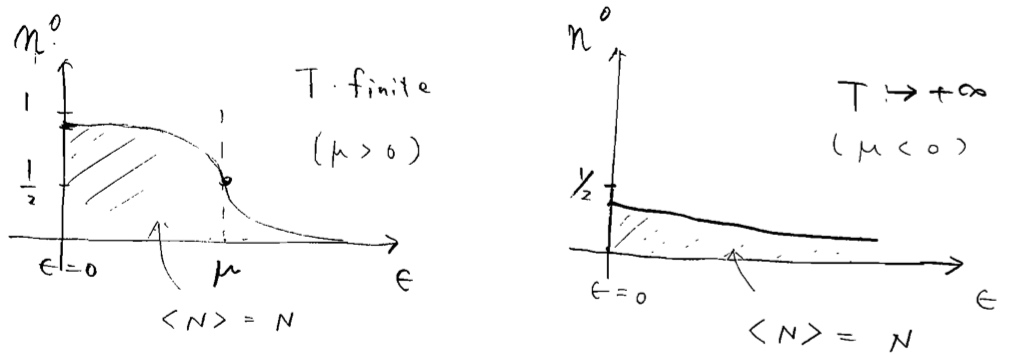
\includegraphics[width=\textwidth]{fig4-9-8}
 In this limit, the momentum integral appearing in the zero-th order polarisation part can be evaluated.
%p813
\begin{equation}
\begin{aligned}
F^0(\mathbf k,\omega+i\eta)&=-2\int \frac{d^3\mathbf q}{(2\pi)^3} n^0_{\mathbf q+\frac{\mathbf k}{2}} \left[ \frac{1}{\hbar \omega-\frac{\hbar^2}{m} \mathbf q\cdot\mathbf k+i\eta}-\frac{1}{\hbar \omega+\frac{\hbar^2}{m} \mathbf q\cdot\mathbf k+i\eta} \right]\\
&=-2e^{\beta\mu} \int \frac{d^3\mathbf q}{(2\pi)^3}e^{-\beta\hbar^2 \frac{\left(\mathbf q+\frac{\mathbf k}{2}\right)^2}{2m}}[...]
\end{aligned}
\end{equation}
we first evaluate this $3$-$d$ $\mathbf q$-integral in terms of the cylindrical polar coordinate, where polar axis is taken along $\hat{\mathbf k}$\\
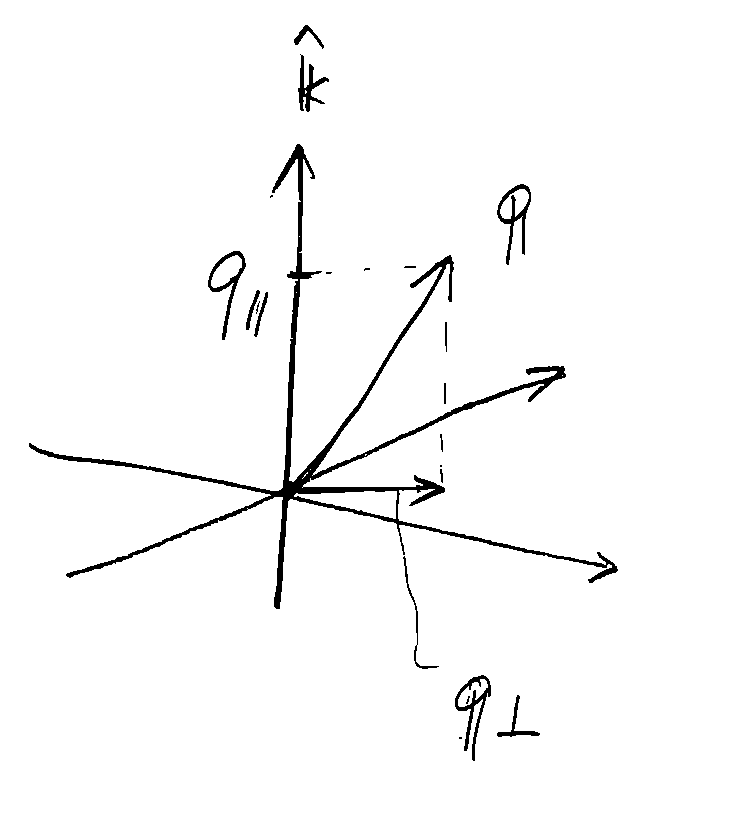
\includegraphics[width=0.4\textwidth]{fig4-9-9}\\
\[
\begin{aligned}
\int \frac{d^3\mathbf q}{(2\pi)^3}&=\int \frac{d^3\mathbf q_\parallel}{(2\pi)^3} \int \frac{d^3\mathbf q_\perp}{(2\pi)^3}\\
\left(\mathbf q+\frac{\mathbf k}{2}\right)^2&=q_\parallel^2+|\mathbf q_\perp|^2+\frac{k^2}{4}+\mathbf q\cdot\mathbf k\\
&=q_\parallel^2+|\mathbf q_\perp|^2+\frac{k^2}{4}+q_\parallel\cdot\mathbf k
\end{aligned}
\]
\[
\begin{aligned}
F^0(\mathbf k,\omega+i\eta)&=-2e^{\beta\mu} \int \frac{d^2\mathbf q_\perp}{(2\pi)^2}e^{-\beta\hbar\frac{|\mathbf q_\perp|^2}{2m}}\\
&\quad \int_{-\infty}^{+\infty} \frac{d q_\parallel}{2\pi} e^{-\beta\hbar^2 \frac{\left(q_\parallel+\frac{ k}{2}\right)^2}{2m}}
\left[ \frac{1}{\hbar \omega-\frac{\hbar^2}{m} q_\parallel k+i\eta}-\frac{1}{\hbar \omega+\frac{\hbar^2}{m}  q_\parallel  k+i\eta} \right]\\
%p814
\left( \int dxdy\ e^{-\alpha(x^2+y^2)}\right. &=\left.2\pi \int_0^{+\infty} rdr\ e^{-\alpha r^2}=\frac{\pi}{\alpha} \right)\\
F^0(\mathbf k,\omega+i\eta)&=-2e^{\beta\mu} \cancelto{\lambda^{-2}}{\left( \frac{m}{2\pi\beta\hbar} \right)} \int_{-\infty}^{+\infty} \frac{d q_\parallel}{2\pi} e^{-\beta\hbar^2 \frac{\left(q_\parallel+\frac{ k}{2}\right)^2}{2m}}
\left[ \frac{1}{\hbar \omega-\frac{\hbar^2}{m} q_\parallel  k+i\eta}-\frac{1}{\hbar \omega+\frac{\hbar^2}{m}  q_\parallel  k+i\eta} \right]
\end{aligned}
\]
where $\lambda=\left( \frac{2\pi\beta\hbar}{m} \right)^{1/2}$ denote the thermal wavelength.
\begin{equation}
F^0(\mathbf k,\omega+i\eta)\equiv F^0_1(\mathbf k,\omega)+iF^0_2(\mathbf k,\omega)
\end{equation}
\begin{equation}
F^0_1(\mathbf k,\omega)=-2e^{\beta\mu} {\lambda^{-2}} \int_{-\infty}^{+\infty} \frac{d q_\parallel}{2\pi} e^{-\beta\hbar^2 \frac{\left(q_\parallel+\frac{ k}{2}\right)^2}{2m}}
\left[ \frac{P}{\hbar \omega-\frac{\hbar^2}{m} (q_\parallel+ k/2)k+\frac{\hbar^2}{m}\frac{k^2}{2}}-\frac{P}{\hbar \omega+\frac{\hbar^2}{m} (q_\parallel+ k/2)k-\frac{\hbar^2}{m}\frac{k^2}{2}} \right]
\end{equation}
%p815
Introducing a new integral variable
\[
y=\left( \frac{\beta\hbar^2}{2m} \right)^{1/2},\quad \frac{\hbar^2}{2m}(q_\parallel+k/2) \left( \frac{2\hbar^2}{\beta m} \right)^{1/2} y
\]
\begin{equation}
\begin{aligned}
F^0_1(\mathbf k,\omega)&=-2e^{\beta\mu} {\lambda^{-2}} \left( \frac{2m}{\beta\hbar^2}^{1/2} \right) \frac{1}{2\pi} \int_{-\infty}^{+\infty} dy e^{-y^2}\\
&\quad \frac{1}{k} \left[ \frac{P}{\left( \hbar \frac{\omega}{k}+\frac{\hbar^2k}{2m} \right)-\frac{\hbar^2}{m}(q_\parallel+k/2)=\left( \frac{2\hbar^2}{\beta m} \right)^{1/2} y}-\frac{P}{\left( \hbar \frac{\omega}{k}-\frac{\hbar^2k}{2m} \right)+\frac{\hbar^2}{m}(q_\parallel+k/2)=\left( \frac{2\hbar^2}{\beta} \right)^{1/2} y} \right]\\
&=-\cancel{2} e^{\beta\mu} {\lambda^{-2}} \left( \frac{\cancel{2}m}{\cancel{\beta}\hbar^2}^{1/2} \right) \frac{1}{\cancel{2}\pi} \frac{1}{k} \left( \frac{\cancel{\beta} m}{\cancel{2}\hbar^2} \right)^{1/2} \int_{-\infty}^{+\infty} dy e^{-y^2}\\
&\quad \left[ \frac{P}{\left(\frac{\beta m}{m}\right)^{1/2} \left( \frac{\omega}{k}+\frac{\hbar k}{2m} \right)-y}-\frac{P}{\left(\frac{\beta m}{m}\right)^{1/2} \left( \frac{\omega}{k}-\frac{\hbar k}{2m} \right)-y} \right]\\
&-\cancel{2}e^{\beta\hbar} \frac{\lambda^{-2}}{\cancel{2}\sqrt \pi k} \frac{m}{\hbar^2} \left[ \Phi \left(\left(\frac{\beta m}{2}\right)^{1/2} \left( \frac{\omega}{k}+\frac{\hbar k}{2m} \right)\right)- \Phi \left(\left(\frac{\beta m}{2}\right)^{1/2} \left( \frac{\omega}{k}-\frac{\hbar k}{2m} \right)\right) \right]
\end{aligned}
\end{equation}
%p816
where 
\begin{equation}
\Phi(x)=\frac{1}{\sqrt \pi} \int_{-\infty}^{+\infty} dy \frac{e^{-y^2}}{x-y}
\end{equation}
is called as (real part of) the plasma dispersion function.
 Within the lowest order in the interaction potential, the chemical potential is given by the total number of particle $N$ or particle density $n=\frac{N}{V}$ as follows
\begin{equation}
e^{\beta\mu}=\frac{1}{2}n\lambda^3
\end{equation}
(an ideal electron gas in the classical limit)\\
\rule{\textwidth}{0.1mm}\\
\[
\frac{N}{V}=\frac{\cancel{2}}{\cancel{4}\pi^2} \left( \frac{2m}{\hbar^2} \right)^{3/2} \int_0^{+\infty} d\epsilon \epsilon^{1/2} e^{-\beta(\epsilon-\mu)}
\]
\[
\begin{aligned}
n&=\frac{1}{2\pi^2} \left(\frac{2m}{\hbar^2}\right)^{3/2} e^{\beta\mu} \cancelto{=\frac{\sqrt \pi}{2}\frac{1}{\beta^{3/2}}}{\int_0^{+\infty} d\epsilon \epsilon^{1/2} e^{-\beta\epsilon}}\\
&=\frac{1}{4\pi^{3/2}\beta^{3/2}} \left(\frac{2m}{\hbar^2}\right)^{3/2} e^{\beta\mu} \\
%p817
&=\frac{1}{\sqrt 2} \left( \frac{m}{\pi \beta \hbar^2} \right)^{3/2} e^{\beta \mu}=2 \left( \frac{m}{2\pi \beta \hbar^2} \right)^{3/2} e^{\beta \mu}\\
&=2\lambda^{-3}e^{\beta\mu}\\
\therefore& \to e^{\beta\mu}=\frac{1}{2}n\lambda^3
\end{aligned}
\]
\rule{\textwidth}{0.1mm}\\
In terms of this, the real part is given by
\begin{equation}
\begin{aligned}
F^0_1(\mathbf k,\omega)&=-\frac{n\lambda}{2\sqrt \pi k}\frac{m}{\hbar^2} [\Phi(..+..)-|phi(..-..)]\\
&=\frac{1}{2\cancel{\sqrt \pi}} \frac{n}{k} \left( \frac{2\cancel{\pi}\beta\hbar^2}{m} \right)^{1/2} [...]\\
&=\frac{n}{\hbar k} \left( \frac{1}{2}\beta m \right)^{1/2} \left[ \Phi \left(\left(\frac{\beta m}{2}\right)^{1/2} \left( \frac{\omega}{k}+\frac{\hbar k}{2m} \right)\right)- \Phi \left(\left(\frac{\beta m}{2}\right)^{1/2} \left( \frac{\omega}{k}-\frac{\hbar k}{2m} \right)\right) \right]\\
\left( with\ \Phi(x)=\frac{1}{\sqrt \pi} \int_{-\infty}^{+\infty} dy \frac{e^{-y^2}}{x-y} \right)
\end{aligned}
\end{equation}
%p818
On the one hand, the imaginary part is calculated as follows:
\begin{equation}
F^0_2(\mathbf k,\omega)=-2e^{\beta\mu}\lambda^{-2}\int_{-\infty}^{+\infty} \frac{d q_\parallel}{2\pi}e^{-\beta\hbar^2\frac{q_\parallel+\frac{k}{2}}{2m}} (-\pi)
\left[ \delta(\hbar \omega-\frac{\hbar^2}{m}q_\parallel k)-\delta(\hbar \omega+\frac{\hbar^2}{m}q_\parallel k) \right]\\
\end{equation}
\begin{equation}
\begin{aligned}
F^0_2(\mathbf k,\omega)&=e^{\beta\mu}\lambda^{-2}\frac{m}{\hbar^2 k} \int_{-\infty}^{+\infty} \frac{d q_\parallel}{2\pi}e^{-\beta\hbar^2\frac{q_\parallel+\frac{k}{2}}{2m}} (-\pi)
\left[ \delta(q_\parallel -\frac{m\omega}{\hbar k})-\delta(q_\parallel +\frac{m\omega}{\hbar k}) \right]\\
&=e^{\beta\mu}\lambda^{-2}\frac{m}{\hbar^2 k} \left\{ e^{-\beta\hbar^2 \frac{1}{2m}\left( \frac{m\omega}{\hbar k}+\frac{k}{2} \right)}-e^{-\beta\hbar^2 \frac{1}{2m}\left( -\frac{m\omega}{\hbar k}+\frac{k}{2} \right)} \right\}\\
&=...\\
&=-\frac{n\beta\omega}{k} \left( \frac{1}{2} \pi \beta m\right)^{1/2} \exp\left[ -\frac{\beta m\omega^2}{2k^2}-\frac{\beta\hbar^2 k^2}{8m} \right] \frac{\sinh \left( \frac{1}{2} \beta \hbar \omega \right)}{ \left( \frac{1}{2} \beta \hbar \omega \right)}
\end{aligned}
\end{equation}
%p819
To summarise, we have the retarded density$^2$ correlation function within the lowest-order approximation to the proper polarisation part:
\begin{equation}
D^R_{ring}(\mathbf k,\omega)=\frac{\hbar F^0_1(\mathbf k,\omega)+i\hbar F^0_2(\mathbf k,\omega)}{1-\left(F^0_1(\mathbf k,\omega)+iF^0_2(\mathbf k,\omega)\right)V_0(\mathbf k)}
\end{equation}
where these two real-valued functions are evaluated in the high-temperature limit:
\begin{equation}\label{eq4.9.40}
F^0_1(\mathbf k,\omega)=\frac{n}{\hbar |k|}  \left( \frac{1}{2} \beta m \right)^{1/2} 
\left[ \Phi \left(\left(\frac{\beta m}{2}\right)^{1/2} \left( \frac{\omega}{k}+\frac{\hbar k}{2m} \right)\right)- \Phi \left(\left(\frac{\beta m}{2}\right)^{1/2} \left( \frac{\omega}{k}-\frac{\hbar k}{2m} \right)\right) \right]
\end{equation}
\begin{equation}\label{eq4.9.41}
F^0_2(\mathbf k,\omega)=-\frac{n\beta\omega}{k} \left( \frac{1}{2} \pi \beta m\right)^{1/2} \exp\left[ -\frac{\beta m\omega^2}{2k^2}-\frac{\beta\hbar^2 k^2}{8m} \right] \frac{\sinh \left( \frac{1}{2} \beta \hbar \omega \right)}{ \left( \frac{1}{2} \beta \hbar \omega \right)}
\end{equation}
where $\Phi(x)$ is the real part of the Plasma dispersion function
\begin{equation}
\Phi(x)=\frac{1}{\sqrt \pi} \int_{-\infty}^{+\infty} dy \frac{e^{-y^2}}{x-y}
\end{equation}
%p820
 Asymptotic forms of this function can be evaluated in two limiting situations:
\begin{equation}
\Phi(x)=
\left\{
\begin{aligned}
&\frac{1}{x}(1-\frac{1}{2x^2}+...)\qquad x\to+\infty\\
&2x(1-\frac{2x^2}{3}+...)\qquad x\to 0
\end{aligned}
\right.
\end{equation}
 Using these results, let us first study the screening effect in an electron gas at the high temperature limit.
 To be specific, we consider that the external perturbation is a positive point-charge with $Ze$ charges.
\begin{equation}
\varphi^{ex}(\mathbf x,t)=\frac{Ze}{x}
\end{equation}
Or equivalently
\begin{equation}\tag{4.9.44'}
\varphi^{ex}(\mathbf k,\omega)=\frac{8\pi^2Ze}{|\mathbf k|^2} \delta(\omega)
\end{equation}
%p788
The charge density induced by this point charge is given by eq.(\ref{eq4.9.10}), within the linear response theory.
\begin{equation}\label{eq4.9.45}
\begin{aligned}
\delta\langle\rho(\mathbf x,t)\rangle&=-e\delta\langle n(\mathbf x,t)\rangle\\
&=\frac{e^2}{\hbar}\int \frac{d^3\mathbf k}{(2\pi)^3} \int\frac{d\omega}{2\pi} e^{i\mathbf k\cdot \mathbf x-i\omega t}D^R(\mathbf k,\omega)\varphi^{ex}(\mathbf k,\omega)\\
&=\frac{Ze}{\hbar} \int \frac{d^3\mathbf k}{(2\pi)^3} D^R(\mathbf k,0) \cancelto{V_0(\mathbf k)}{\frac{4\pi e^2}{|\mathbf k|^2}} e^{i\mathbf k\cdot \mathbf x}\\
&=Ze\int \frac{d^3\mathbf k}{(2\pi)^3}\frac{F^0_1(\mathbf k,0)V_0(\mathbf k)}{1-F^0_1(\mathbf k,0)V_0(\mathbf k)} e^{i\mathbf k\cdot \mathbf x}\\
&(F_2^0(\mathbf k,0)=0)
\end{aligned}
\end{equation}
From eq.(\ref{eq4.9.40}), we have
\begin{equation}
\begin{aligned}
V_0(\mathbf k)F^0_1(\mathbf k,0)&=-\frac{8\pi e^2n}{\hbar k^3} \left( \frac{1}{2}\beta m \right)^{1/2} \Phi\left( \cancelto{\lambda\frac{k}{4\sqrt \pi}}{\left( \frac{\beta m}{2} \right)^{1/2}}  \frac{\hbar|\mathbf k|}{2m}\right)\\
&=-\frac{8\pi e^2n}{\hbar k^2} \left( \frac{1}{2}\beta m \right)^{1/2} \frac{\lambda}{\lambda k}\Phi\left( \frac{\lambda k}{4\sqrt\pi} \right)\\
&=-\frac{8\pi e^2n}{\cancel{\hbar} k^2} \left( \frac{1}{\cancel{2}}\beta \cancel{m} \right)^{1/2} \left( \frac{\cancel{2}\pi \cancel{\hbar^2} \beta}{\cancel{m}} \right)^{1/2} \frac{1}{\lambda k} \Phi\left( \frac{\lambda k}{4\sqrt\pi} \right)\\
%p789
&=-\frac{8\pi}{k^2}(e^2n\beta)\sqrt\pi\frac{1}{\lambda k}\Phi\left( \frac{\lambda k}{4\sqrt\pi} \right)\\
&=-\frac{1}{k^2}(4\pi e^2n\beta)2\sqrt\pi\frac{1}{\lambda k}\Phi\left( \frac{\lambda k}{4\sqrt\pi} \right)\\
&\equiv -\frac{1}{k^2}q_D^2\cancelto{g_1(\lambda k)}{2\sqrt\pi\frac{1}{\lambda k}\Phi\left( \frac{\lambda k}{4\sqrt\pi} \right)}
\end{aligned}
\end{equation}
where we define the Debye shielding length $q_D^{-1}$ as follows
\begin{equation}
q_D=\sqrt{4\pi e^2 n\beta}
\end{equation}
substituting this into eq.(\ref{eq4.9.45}), we have
\begin{equation}
\begin{aligned}
\delta\langle\rho(\mathbf x,t)\rangle&=-Ze\int \frac{d^3\mathbf k}{(2\pi)^3}e^{i\mathbf k\cdot\mathbf x}\frac{\frac{q_D^2}{k^2}g_1(\lambda k)}{1+\frac{q_D^2}{k^2}g_1(\lambda k)}\\
&=-Ze\int \frac{d^3\mathbf k}{(2\pi)^3}e^{i\mathbf k\cdot\mathbf x}\frac{q_D^2 g_1(\lambda k)}{k^2+q_D^2 g_1(\lambda k)}
\end{aligned}
\end{equation}
 As in the zero-temperature case, the total induced charge is $-Ze$, so that the impurity is completely screened.\\
\begin{equation}
\int \delta\langle\rho(\mathbf x,t)\rangle=-Ze
\end{equation}
Since the function $g_1(z)$ is an entire function (holomorphic in the entire complex $z$-plane).
%790
 The asymptotic behaviour of the r.h.s can be evaluated by the following approximation:
\begin{equation}
g_1(\lambda k)\approx 1+O((\lambda k)^2)
\end{equation}
 Retaining only the first term, we have Thomas-Fermi result
\begin{equation}
\delta\langle\rho(\mathbf x,t)\rangle\approx -Ze\int \frac{d^3\mathbf k}{(2\pi)^3}e^{i\mathbf k\cdot\mathbf x}\frac{q_D^2}{k^2+q_D^2}=-Z e q_D^2\frac{e^{-q_D x}}{4\pi x}\quad(|\mathbf x|\to+\infty)
\end{equation}
 This expression suggests that $q_D^{-1}$ is nothing but the screening length.
 In the zero-temperature case, the asymptotic behaviour of the induced charge exhibit an oscillating behaviour due to the presence of the Fermi surface.
 In the high-temperature case, the sharp drop of the distribution function at the Fermi surface is completely smeared out by the temperature effect.
 As a result, the asymptotic behaviour of the induced charge density does not exhibit the oscillating behaviour at the high temperature limit.
%p821
 Using the result given in eqs(...), let us next examine the plasma oscillation in the high temperature limit.
 As we did in the zero-temperature case, we consider the charge density induced by an impulsive perturbation
\begin{equation}
\varphi^{ex}(\mathbf x,t)=\varphi_0 e^{i\mathbf k\cdot\mathbf x}\delta(t)
\end{equation}
Or equivalently
\begin{equation}\tag{4.9.52'}
\varphi^{ex}(\mathbf q,\omega)=\varphi_0 (2\pi)^3 \delta(\mathbf q-\mathbf k)
\end{equation}
 Within the linear response theory, the induced charge density has the same momentum $\mathbf k$:
\[
\delta\langle n(\mathbf x,t)\rangle=-\frac{e}{\hbar}\varphi_0e^{i\mathbf k\cdot\mathbf x} \int_{-\infty}^{+\infty}\frac{d\omega}{2\pi}e^{-i\omega t}D^R(\mathbf k,\omega)
\]
 Within the lowest order approximation to the proper polarization part, the right hand side is given by
%p822
\begin{equation}
=-e\varphi_0 e^{i\mathbf k\cdot \mathbf x} \int \frac{d\omega}{2\pi} e^{-i\omega t} \frac{F_1^0(\mathbf k,\omega)+iF_2^0(\mathbf k,\omega)}{1-V_0(\mathbf k)F_1^0(\mathbf k,\omega)-iV_0(\mathbf k)F_2^0(\mathbf k,\omega)}
\end{equation}
where the function $F_1^0$ \& $F_2^0$ were calculated in the high-temperature limit as in eqs.(\ref{eq4.9.40}),(\ref{eq4.9.41}).
 As we have already discussed in sec.3-2, this expression suggests that the plasma oscillation frequency and its life time are determined by pole of the integrand in the complex-$\omega$ plane.
 Since the numerator is an entire function of the complex variable $\omega$, the pole is encoded as the zero of the denominator.
%p823
\begin{equation}
1-V_0(\mathbf k)F_1^0(\mathbf k,\Omega_{\mathbf k}-i\gamma_{\mathbf k}) -iV_0(\mathbf k)F_2^0(\mathbf k,\Omega_{\mathbf k}-i\gamma_{\mathbf k}) 
\end{equation}
 We can solve this equation approximately, by assuming that the damping coefficient $\gamma_{\mathbf k}$ is much smaller that the plasma oscillation frequency $\gamma_{\mathbf k}\ll \Omega_{\mathbf k}$.
 This approximation will be a posteriori justified for sufficiently small $\mathbf k$.
 When $\gamma_{\mathbf k}\ll \Omega_{\mathbf k}$, we can expand this equation in small $\gamma_{\mathbf k}$:
 the zero-th order in $\gamma_{\mathbf k}$
\begin{equation}\label{eq4.9.55}
1-V_0(\mathbf k)F_1^0(\mathbf k,\Omega_{\mathbf k})=0
\end{equation}
 the first order in $\gamma_{\mathbf k}$.
%p824
\begin{equation}
i\gamma_{\mathbf k}\cancel{V_0(\mathbf k)}\left.\frac{\partial F_1^0(\mathbf k,\omega)}{\partial \omega}\right|_{\omega=\Omega_{\mathbf k}}-i\cancel{V_0(\mathbf k)} F_2^0(\mathbf k,\Omega_{\mathbf k})
\end{equation}
 ...
 From eq.(\ref{eq4.9.55}), we can determine the plasma frequency as a function of the momentum $\mathbf k$.
 For sufficiently small $\mathbf k$ (with fixed $\omega$), $F_1^0(\mathbf k,\omega)$ can be expanded in large $\frac{\omega}{k}$:
\begin{equation}
\begin{aligned}
F_1^0(\mathbf k,\omega)&=-\frac{n}{\hbar k}\left( \frac{1}{2}\beta m \right)^{1/2} \left\{ \frac{1}{\left(\frac{1}{2}m\beta\right)^{1/2} \left( \frac{\omega}{k}+\frac{\hbar k}{2m} \right)^2}  \left(1+\frac{1}{2} \frac{1}{\frac{1}{2}m\beta \left( \frac{\omega}{k}+\frac{\hbar k}{2m} \right)^2} +...\right)  \right.\\
&\qquad\qquad\qquad\qquad-\left.\frac{1}{\left( \frac{1}{2}m\beta\right)^{1/2} \left( \frac{\omega}{k}-\frac{\hbar k}{2m} \right)^2} \left(1+\frac{1}{2} \frac{1}{\frac{1}{2}m\beta \left( \frac{\omega}{k}-\frac{\hbar k}{2m} \right)^2} +...\right)  \right\}\\
&=\frac{nk^2}{m\omega^2}\left( 1+\frac{3k^2}{\beta m\omega^2}+... \right)\qquad for\ small\ \frac{k}{\omega}
\end{aligned}
\end{equation}
%p825
 Substituting this asymptotic form into eq.(t), we obtain
\begin{equation}
1=\frac{4\pi ne^2}{m\Omega_{\mathbf k}^2}\left( 1+\frac{3k^2}{\beta m\Omega_{\mathbf k}^2}+... \right)
\end{equation}
 Solving this in favor of $\Omega_{\mathbf k}$, we have 
\begin{equation}
\Omega_{\mathbf k}=\pm \sqrt{\frac{4\pi ne^2}{m}}\left( 1+\frac{3}{2}\left( \frac{q}{q_D} \right)^2+... \right)
\end{equation}
where $q_D^{-1}$ is the Debye Schielding length.
 Since $\beta\hbar \Omega_{\mathbf k}\fallingdotseq\beta\hbar\left(\frac{4\pi ne^2}{m}\right)^{1/2}=\frac{1}{\sqrt{2\pi}}q_D\lambda\ll 1$
\[
\left( q_D\lambda=(4\pi ne^2\beta)^{1/2}\left( \frac{2\pi\hbar^2\beta}{m} \right)^{1/2}=(2\pi)^{1/2}\beta\hbar\left(\frac{4\pi ne^2}{m}\right)^{1/2} \right)
\]
in the high-temperature limit, we can approximate $F_2^0(\mathbf k,\Omega_{\mathbf k})$ as follows
\begin{equation}
F_2^0(\mathbf k,\Omega_{\mathbf k})\approx \frac{n\beta\Omega_{\mathbf k}}{k} \left( \frac{\pi}{2}\beta m \right)^{1/2} \exp \left( -\frac{\beta m\Omega_{\mathbf k}^2}{2k^2} \right)
\end{equation}
%p826
 The derivative of $F_1^0$ with respect to $\Omega_{\mathbf k}$ is as follows
\[
\frac{\partial F_1(\mathbf k,\omega)}{\partial \omega}=-2\frac{nk^2}{m\omega^3}+...
\]
(for small $\frac{k}{\omega}$)\\
 Substituting these asymptotic forms into eq.(s), we have
\begin{equation}
\begin{aligned}
\gamma_{\mathbf k}&=F_2^0(\mathbf k,\Omega_{\mathbf k})\left. \left[ \frac{\partial F_1(\mathbf k,\omega)}{\partial \omega} \right]^{-1}\right|_{\omega=\Omega_{\mathbf k}}\\
&\fallingdotseq\frac{m\beta \Omega_{pl}^4}{2k^3} \left( \frac{\pi}{2}\beta m \right)^{1/2} \exp\left( -\frac{\beta m\Omega_{pl}^2}{2k^2} \right)\\
&\fallingdotseq\frac{\Omega_{pl}^4}{k^3}(m\beta)^{3/2}\left( \frac{\pi}{8} \right)^{1/2}\exp\left( -\frac{\beta m\Omega_{pl}^2}{2k^2} \right)\\
&=\Omega_{pl}\left( \frac{q_D}{k} \right)^3\left( \frac{\pi}{8} \right)^{1/2}\exp\left( -\frac{1}{2}\left( \frac{q_D}{k} \right)^2 \right)
\end{aligned}
\end{equation}
Because of this exponential factor, this damping coefficient becomes much smaller
%p827
than the plasma frequency for the long wave length limit $k\ll q_D$.
 This weak damping is called as Landau damping.
